\documentclass[12pt]{report}

\usepackage{amsmath}
\usepackage{amssymb}
\usepackage{amsthm}

\usepackage{graphicx}
\graphicspath{ {./} }

\usepackage[utf8]{inputenc}
\usepackage[T1]{fontenc}

\usepackage[inline]{enumitem}

\usepackage{tikz}
\usetikzlibrary{shapes.multipart}
\usetikzlibrary{arrows}
\usetikzlibrary{patterns}

\newtheorem{theorem}{Theorem}
\newtheorem{lemma}{Lemma}
\newtheorem*{prop}{Proposition}
\newtheorem{definition}{Definition}
\newtheorem*{example}{Example}
\newtheorem*{notation}{Notation}
\newtheorem*{cor}{Corollary}
\newtheorem*{rem}{Remark}

\begin{document}

\title{Rational Parking Functions}
\author{Matthieu Josuat-Vergès \and Tessa Lelièvre-Osswald}
\date{August 27, 2020}

\maketitle

\begin{abstract}
    This is an abstract about Rational Parking Functions.
\end{abstract}

\tableofcontents

\chapter{The integer case}

\section{Parking Functions}

\begin{definition}[Parking Function]
    A \emph{parking function} is a sequence of positive integers
    $(a_1, a_2, \ldots, a_n)$
    such that its non-decreasing reordering $(b_1, b_2, \ldots, b_n)$
    has $b_i \leqslant i$ for all $i$.\\
    We denote by $\mathcal{PF}_n$ the set of parking functions of length $n$.
    $$\mathcal{PF} = \bigcup_{n > 0}{\mathcal{PF}_n}$$.
\end{definition}

\begin{example}
    \begin{align*}
    &f_1 = (7, 3, 1, 4, 2, 5, 2) \in \mathcal{PF}_7\\
    &f_2 = (7, 3, 1, 4, 2, 5, 4) \notin \mathcal{PF}_7\\
    \end{align*}
\end{example}

\begin{theorem}
    Let $pf_n$ be the cardinal of $\mathcal{PF}_n$.
    We have $$pf_n = (n + 1)^{n-1}$$.
\end{theorem}

\begin{example}[$n = 1, 2, 3$]
    ~\\
    \begin{itemize*}
            \item $n = 1$ \  $:$ \  $pf_1 = 1$\\
            \subitem $(1)$\\
            \item $n = 2$ \  $:$ \  $pf_2 = 3$\\
            \subitem $(1, 1)$
            \subitem $(1, 2)$
            \subitem $(2, 1)$\\
            \item $n = 3$ \  $:$ \  $pf_3 = 16$\\
            \subitem $(1, 1, 1)$
            \subitem $(1, 1, 2)$
            \subitem $(1, 1, 3)$
            \subitem $(1, 2, 1)$
            \subitem $(1, 2, 2)$
            \subitem $(1, 2, 3)$
            \subitem $(1, 3, 1)$
            \subitem $(1, 3, 2)$
            \subitem $(2, 1, 1)$
            \subitem $(2, 1, 2)$
            \subitem $(2, 1, 3)$
            \subitem $(2, 2, 1)$
            \subitem $(2, 3, 1)$
            \subitem $(3, 1, 1)$
            \subitem $(3, 1, 2)$
            \subitem $(3, 2, 1)$\\
    \end{itemize*}
\end{example}

\subsection{Primitive parking functions}

\begin{definition}[Primitive]
    A parking function $(a_1, a_2, \ldots, a_n)$ is said \emph{primitive} if
    it is already in non-decreasing order. \\
    We denote by $\mathcal{PF'}_n$ the set of primitive parking functions of length $n$.
    $$\mathcal{PF'} = \bigcup_{n > 0}{\mathcal{PF'}_n}$$
    
\end{definition}

\begin{example}
    \begin{align*}
        &f_1 = (1, 2, 2, 3) \in \mathcal{PF'}_4\\
        &f_2 = (1, 2, 3, 2) \notin \mathcal{PF'}_4
         \text{, even though } f_2 \in \mathcal{PF}_4\\
    \end{align*}
\end{example}

\begin{theorem}
    Let $pf'_n$ be the cardinal of $\mathcal{PF'}_n$.
    We have $$pf'_n = \frac{1}{n + 1} \binom{2n}{n}$$
    which is the $n^{th}$ Catalan number $Cat(n)$.
\end{theorem}

\begin{example}[$n = 1, 2, 3$]
    ~\\
    \begin{itemize*}
        \item $n = 1$ \  $:$ \  $pf'_1 = 1$\\
        \subitem $(1)$\\
        \item $n = 2$ \  $:$ \  $pf'_2 = 2$\\
        \subitem $(1, 1)$
        \subitem $(1, 2)$\\
        \item $n = 3$ \  $:$ \  $pf'_3 = 5$\\
        \subitem $(1, 1, 1)$
        \subitem $(1, 1, 2)$
        \subitem $(1, 1, 3)$
        \subitem $(1, 2, 2)$
        \subitem $(1, 2, 3)$\\
    \end{itemize*}
\end{example}

\section{Non-crossing Partitions}

\begin{definition}[Non-crossing Partition]
    A \emph{non-crossing partition} of a \emph{totally
    ordered} set $E$ is
    a set partition $P = \{E_1, E_2, \ldots, E_k\}$ such that
    if $a, c \in E_i$, $b, d \in E_j$, and $i \neq j$, then
    we do \emph{not} have $a < b < c < d$, nor $a > b > c > d$.\\
    We denote by $\mathcal{NC}_n$ the set of non-crossing partitions
    of $\{1, 2, \ldots, n\}$.
    $$\mathcal{NC} = \bigcup_{n > 0}{\mathcal{NC}_n}$$
\end{definition}

From this point, we assume that every partition $P = \{B_1, \ldots, B_l\}$
is \emph{sorted} such that :\\
\begin{itemize*}
    \item For each block $B_i = \{b_1, \ldots, b_k\} \in P$,
        $b_1 < \ldots < b_k$\\
    \item $min (B_1) < \ldots < min (B_k)$\\
\end{itemize*}

\begin{notation}
    $[n] = \{1, 2, \ldots, n\}$
\end{notation}

\begin{example}[$E = \lbrack 6 \rbrack $]
    \begin{align*}
        &P_1 = \{\{1, 2, 5\}, \{3, 4\}, \{6\}\} \in \mathcal{NC}_6\\
        &P_2 = \{\{1, 2, 4\}, \{3, 5\}, \{6\}\} \notin \mathcal{NC}_6
    \end{align*}
\end{example}

\begin{theorem}
    Let $nc_n$ be the cardinal of $\mathcal{NC}_n$.
    We have $$nc_n = \frac{1}{n + 1} \binom{2n}{n}$$
    which is again the $n^{th}$ Catalan number
    $Cat(n)$.
\end{theorem}

\begin{example}[$n = 1, 2, 3$]
    ~\\
    \begin{itemize*}
        \item $n = 1$ \  $:$ \  $nc_1 = 1$\\
        \subitem $\{\{1\}\}$\\
        \item $n = 2$ \  $:$ \  $nc_2 = 2$\\
        \subitem $\{\{1, 2\}\}$
        \subitem $\{\{1\}, \{2\}\}$\\
        \item $n = 3$ \  $:$ \  $nc_3 = 5$\\
        \subitem $\{\{1, 2, 3\}\}$
        \subitem $\{\{1\}, \{2, 3\}\}$
        \subitem $\{\{1, 3\}, \{2\}\}$
        \subitem $\{\{1, 2\}, \{3\}\}$
        \subitem $\{\{1\}, \{2\}, \{3\}\}$\\
    \end{itemize*}
\end{example}

\begin{prop}
    This means we can create a \emph{bijection} between
    $\mathcal{PF'}_n$ and $\mathcal{NC}_n$.
\end{prop}

\begin{proof}
    ~\\
\begin{itemize}
    \item $\mathcal{NC}_n \to \mathcal{PF'}_n$ :
    For each block $B$ in the non-crossing partition, take
    $i = min (B)$, and let $k_i = size (B)$.\\
    $k_i = 0$ if $i$ is not the minimum of a block.\\
    The corresponding parking function is
    $(\underbrace{1, \ldots, 1}_{k_1}, \underbrace{2, \ldots,
    2}_{k_2}, \ldots, \underbrace{n, \ldots, n}_{k_n})$.\\
    \item $\mathcal{PF'}_n \to \mathcal{NC}_n$ :
    For each $i$ in $[n]$, if $i$ appears $n_i$ times in the
    parking function, $B_i$ will be of size $n_i$ with minimum
    element $i$.
    There is a unique set partition $\displaystyle P = \bigcup_{i}{B_i}$
    of $[n]$ respecting these conditions that is non-crossing :
    for each minimum $i$ in \emph{decreasing order}, add
    the $n_i$ first free elements of
    $[i+1, i+2, \ldots, n, 1, \ldots, i-1]$ to $B_i$.
\end{itemize}
\end{proof}

\begin{example}[$n = 6$]
    \begin{align*}
        &P = \{\{1, 2, 5\}, \{3, 4\}, \{6\}\}
        &f = (1, 1, 1, 3, 3, 6)\\
    \end{align*}
\end{example}

\begin{cor}
    A non-crossing partition can be represented by the minimums
    and sizes of its blocks.
\end{cor}

\begin{example}
    $\{\{1, 2, 5\}, \{3, 4\}, \{6\}\}$ can be represented by
    the following dictionnary :\\
    \begin{itemize*}
        \item 1 : 3\\
        \item 3 : 2\\
        \item 6 : 1\\
    \end{itemize*}
\end{example}

A non-crossing partition of $[n]$ can be represented graphically
on a regular $n$-vertices polygon, with vertices labeled from $1$
to $n$ clockwise. We then represent each block $B = \{b_1, \ldots, b_k\}$
by the convex hull of $\{b_1, \ldots, b_k\}$.\\

\begin{example}[$P = \{\{1, 2, 5\}, \{3, 4\}, \{6\}\}$]
    ~\\
    \begin{center}
        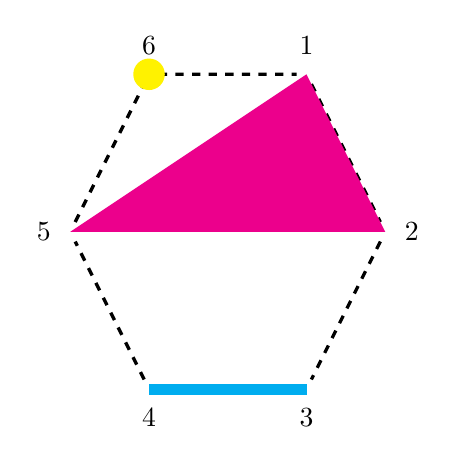
\begin{tikzpicture}[scale=1]
            \node [label = above : {$1$}] (1)
                at (4,5) {};
            \node [label = right : {$2$}] (2)
                at (5,3) {};
            \node [label = below : {$3$}] (3)
                at (4,1) {};
            \node [label = below : {$4$}] (4)
                at (2,1) {};
            \node [label = left : {$5$}]  (5)
                at (1,3) {};
            \node [label = above : {$6$}] (6)
                at (2,5) {};
            \draw [dashed][very thick]
            (1) -- (2) -- (3) -- (4)
                -- (5) -- (6) -- (1);
            \fill [color = magenta] (4,5) -- (5,3)
                -- (1,3) -- cycle;
            \draw [color = cyan][line width = 4pt] 
                (4,1) -- (2,1);
            \fill [color=yellow] (2,5) circle (0.2);
          \end{tikzpicture}
    \end{center}
    Thus non-crossing meaning the hulls are
    \emph{disjoint}.\\
\end{example}

\begin{example}[Counter-example : $P = \{\{1, 5, 2\},
    \{3, 6\}, \{4\}\}$]
    ~\\
    \begin{center}
        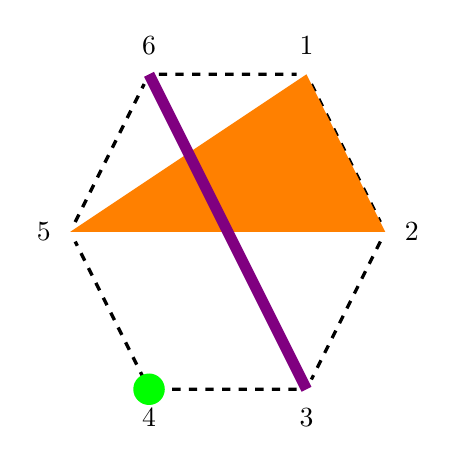
\begin{tikzpicture}[scale=1]
            \node [label = above : {$1$}] (1)
                at (4,5) {};
            \node [label = right : {$2$}] (2)
                at (5,3) {};
            \node [label = below : {$3$}] (3)
                at (4,1) {};
            \node [label = below : {$4$}] (4)
                at (2,1) {};
            \node [label = left : {$5$}]  (5)
                at (1,3) {};
            \node [label = above : {$6$}] (6)
                at (2,5) {};
            \draw [dashed][very thick]
            (1) -- (2) -- (3) -- (4)
                -- (5) -- (6) -- (1);
            \fill [color = orange] (4,5) -- (5,3)
                -- (1,3) -- cycle;
            \draw [color = violet][line width = 4pt] 
                (4,1) -- (2,5);
            \fill [color=green] (2,1) circle (0.2);
          \end{tikzpicture}
    \end{center}
    This partition is \emph{not} non-crossing, as the
    convex hulls of $\{1, 2, 5\}$ and $\{3, 6\}$ are
    \emph{not} disjoint.
\end{example}

\subsection{The non-crossing partitions poset}

\begin{definition}[$\succ$]
    We say that $P$ covers $Q$, written $P \succ Q$,
    if $\exists B_i, B_j \in P$ such that
    $Q = P - \{B_i, B_j\} \cup \{B_i \cup B_j\}$    
\end{definition}

\begin{example}
    $\{\{1, 6\}, \{2, 3\}, \{4, 5\}\} \succ
    \{\{1, 2, 3, 6\}, \{4, 5\}\}$\\
    \begin{itemize*}
        \item $B_i = \{1, 6\}$\\
        \item $B_j = \{2, 3\}$\\
    \end{itemize*}
\end{example}

\begin{prop}
    This covering relation defines the \emph{poset}
    of $\mathcal{NC}_n$.
    We denote by $\mathcal{NCC}_n$ the set of
    \emph{maximal chains} in the poset of $\mathcal{NC}_n$.\\
    $$\mathcal{NCC} = \bigcup_{n > 0}{\mathcal{NCC}_n}$$
\end{prop}

\begin{rem}
    The bottom element of this poset is $\{\{1, \ldots, n\}\}$,
    and the top element is $\{\{1\}, \ldots, \{n\}\}$.
\end{rem}

\begin{theorem}
    Let $ncc_n$ be the cardinal of $\mathcal{NCC}_n$.
    We have $$ncc_n = n^{n - 2}$$.
\end{theorem}

\begin{example}[The poset of $\mathcal{NC}_4$]
    ~\\
    To shorten labels, we represent $\{\{1\}, \{2, 3\},
    \{4\}\}$ by $1|23|4$. \\

    \begin{center}
        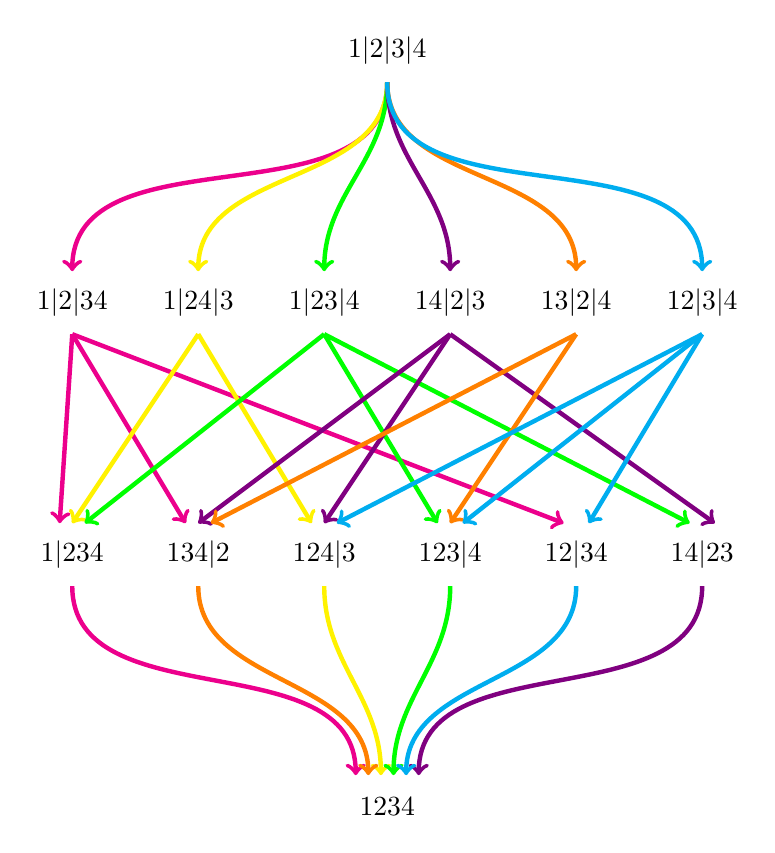
\begin{tikzpicture}[scale = 0.8]
            \node (0)  at (0,0)  {$1234$};
            \node (1)  at (-5,4) {$1|234$};
            \node (2)  at (-3,4) {$134|2$};
            \node (3)  at (-1,4) {$124|3$};
            \node (4)  at (1,4)  {$123|4$};
            \node (5)  at (3,4)  {$12|34$};
            \node (6)  at (5,4)  {$14|23$};
            \node (7)  at (-5,8) {$1|2|34$};
            \node (8)  at (-3,8) {$1|24|3$};
            \node (9)  at (-1,8) {$1|23|4$};
            \node (10) at (1,8)  {$14|2|3$};
            \node (11) at (3,8)  {$13|2|4$};
            \node (12) at (5,8)  {$12|3|4$};
            \node (13) at (0,12) {$1|2|3|4$};
        
            \draw [->][out=-90,in=90, ultra thick] 
                [color=magenta](0,11.5) to (-5,8.5);
            \draw [->][color=magenta, ultra thick]
                (-5,7.5) to (-5.2,4.5);
            \draw [->][color=magenta, ultra thick]
                (-5,7.5) to (-3.2,4.5); 
            \draw [->][color=magenta, ultra thick]
                (-5,7.5) to (2.8,4.5);
            \draw [->][out=-90,in=90, ultra thick] 
                [color=magenta](-5,3.5) to (-0.5,0.5);
        
            \draw [->][out=-90,in=90, ultra thick]
                [color=yellow] (0,11.5) to (-3,8.5);
            \draw [->][color=yellow, ultra thick]
                (-3,7.5) to (-5,4.5);
            \draw [->][color=yellow, ultra thick]
                (-3,7.5) to (-1.2,4.5);
            \draw [->][out=-90,in=90, ultra thick] 
                [color=yellow](-1,3.5) to (-0.1,0.5);
            
            \draw [->][out=-90,in=90, ultra thick]
                [color=green](0,11.5) to (-1,8.5);
            \draw [->][color=green, ultra thick]
                (-1,7.5) to (-4.8,4.5);
            \draw [->][color=green, ultra thick]
                (-1,7.5) to (0.8,4.5);
            \draw [->][color=green, ultra thick]
                (-1,7.5) to (4.8,4.5);
            \draw [->][out=-90,in=90, ultra thick] 
                [color=green](1,3.5) to (0.1,0.5);
        
            \draw [->][out=-90,in=90, ultra thick]
                [color=violet](0,11.5) to (1,8.5);
            \draw [->][color=violet, ultra thick]
                (1,7.5) to (-3,4.5);
            \draw [->][color=violet, ultra thick]
                (1,7.5) to (-1,4.5);
            \draw [->][color=violet, ultra thick]
                (1,7.5) to (5.2,4.5);
            \draw [->][out=-90,in=90, ultra thick] 
                [color=violet](5,3.5) to (0.5,0.5);
        
            \draw [->][out=-90,in=90, ultra thick]
                [color=orange](0,11.5) to (3,8.5);
            \draw [->][color=orange, ultra thick]
                (3,7.5) to (-2.8,4.5);
            \draw [->][color=orange, ultra thick]
                (3,7.5) to (1,4.5);
            \draw [->][out=-90,in=90, ultra thick] 
                [color=orange](-3,3.5) to (-0.3,0.5);
        
            \draw [->][out=-90,in=90, ultra thick]
                [color=cyan](0,11.5) to (5,8.5);
            \draw [->][color=cyan, ultra thick]
                (5,7.5) to (-0.8,4.5);
            \draw [->][color=cyan, ultra thick]
                (5,7.5) to (1.2,4.5);
            \draw [->][color=cyan, ultra thick]
                (5,7.5) to (3.2,4.5);
            \draw [->][out=-90,in=90, ultra thick] 
                [color=cyan](3,3.5) to (0.3,0.5);
        
        \end{tikzpicture}
        ~\\
        ~\\
        There are $4^2 = 16$ different maximal chains,
        and $\frac {1}{5} \binom{8}{4} = \frac{70}{5} = 14$
        elements in this poset.
    \end{center}
\end{example}



\subsection{Kreweras complement}

\begin{definition}[Associated Permutation]
    The \emph{permutation} $\sigma$ associated to a non-crossing
    partition has a cycle $(b_1, \ldots, b_k)$ for each block
    $B = \{b_1, \ldots, b_k\}$ of the partition.
\end{definition}

\begin{example}
    The permutation associated to $\{\{1, 2, 5\}, \{3, 4\}, \{6\}\}$
    is $(1\ 2\ 5)\ (3\ 4)\ (6) = 254316$.
\end{example}

\begin{definition}[Kreweras Complement]
    The \emph{Kreweras complement} $K (P)$ of a non-crossing
    partition $P$ is defined as follows :\\
    \begin{itemize*}
        \item Let $\sigma$ be the permutation associated to $P$\\
        \item Let $\pi$ be the permutation $(n\ n-1\ n-2\
        \ldots\ 3\ 2\ 1) = n123 \ldots n-1$\\
        \item $K (P)$ is the \emph{non-crossing partition}
        associated to $\pi \sigma$.\\
    \end{itemize*}
\end{definition}

\begin{example}[$P = \{\{1, 2, 5\}, \{3, 4\}, \{6\}\}$]
    ~\\
    \begin{itemize*}
        \item $\sigma = (1\ 2\ 5)\ (3\ 4)\ (6) = 254316$\\
        \item $\pi = (6\ 5\ 4\ 3\ 2\ 1) = 612345$\\
        \item $\pi \sigma = 143265 = (1)\ (2\ 4)\ (3)\ (5\ 6)$\\
        \item $K(P) = \{\{1\},\{2, 4\}, \{3\}, \{5, 6\}\}$\\
    \end{itemize*}
\end{example}

\begin{prop}[Kreweras minimums]
        Let $P = \{B_1, \ldots, B_k\}$ be a non-crossing partition.
        Let $K (P) = \{B'_1, \ldots, B'_l\}$ be its Kreweras complement.
        Then $$\bigcup_{1 \leq i \leq l}{min (B'_i)} =
        B_1 \cup \bigcup_{1 < j \leq k}{B_i - {max (B_i)}}$$\\
\end{prop}

\begin{example}[$P = \{\{1, 2, 5\}, \{3, 4\}, \{6\}\}$]
    ~\\
    \begin{itemize}
        \item $K (P) = \{\{1\},\{2, 4\}, \{3\}, \{5, 6\}\}$
        \item $\bigcup{min (B'_i)} = \{1, 2, 3, 5\}$
        \item $B_1\ \cup\ \bigcup{B_i - {max (B_i)}}
        = \{1, 2, 5\} \cup \{3, 4\} - \{4\} \cup \{6\} - \{6\}
        = \{1, 2, 5\} \cup \{3\} \cup \emptyset = \{1, 2, 3, 5\}$\\
    \end{itemize}
\end{example}

\begin{notation}
    $B_{[i]} = $ block containing $i$.
\end{notation}

\begin{prop}[Kreweras block sizes]
    Let $P = \{B_1, \ldots, B_k\}$ be a non-crossing partition.
    Let $K (P) = \{B'_1, \ldots, B'_l\}$ be its Kreweras complement.
    Then the size of the block $B'_i$ is defined as follows :
    \begin{itemize}
        \item Let $m_i$ be the the $i^{th}$ minimum of $K (P)$
        \item Define a \emph{transition} $\phi (e)$ as 
            \subitem Let $j = e + 1$ (or $1$ if $e = n$)
            \subitem $\phi(e) = max (B_{[j]})$
        \item The size of $B'_i$ is $k_{min}$ such that
        $k_{min} = min \{k > 0\ |\ \phi^k (m_i) \in B_{[m_i]}\}$.\\
    \end{itemize}
\end{prop}

\begin{example}[$P = \{\{1, 2, 5\}, \{3, 4\}, \{6\}\}$]
    ~\\
    \begin{itemize}
        \item $mins = \{1, 2, 3, 5\}$
        \item $m_1 = 1$
            \subitem $B_{[1]} = B_1$
            \subitem $max (B_{[2]} = max (B_1) = 5$
            \subitem The size for $m_1$ is $1$.
        \item $m_2$
            \subitem $B_{[2]} = B_1$
            \subitem $max (B_{[3]}) = max (B_2) = 4$
            \subitem $max (B_{[5]}) = max (B_1) = 5$
            \subitem The size for $m_2$ is $2$.
        \item $m_3 = 3$
            \subitem $B_{[3]} = B_2$
            \subitem $max (B_{[4]}) = max (B_2) = 4$
            \subitem The size for $m_3$ is $1$.
        \item $m_4 = 5$
            \subitem $B_{[5]} = B_1$
            \subitem $max (B_{[6]}) = max (B_3) = 6$
            \subitem $max (B_{[1]}) = max (B_1) = 5$
            \subitem The size for $m_4$ is $2$.
    \end{itemize}
\end{example}

\begin{definition}[Mutually Non-crossing Partitions]
    2 partitions $P$ and $Q$ are said
    \emph{mutually non-crossing} if :\\
    \begin{itemize*}
        \item P is non-crossing\\
        \item Q is non-crossing\\
        \item For every block $B_i$ of $P$ and every
        block $B_j$ of $Q$, if $a,c \in B_i$ and
        $b, d \in B_j$, then we can \emph{not} have
        $a < b < c < d$, nor $a > b > c > d$.
    \end{itemize*}    
\end{definition}

\begin{example}[$P = \{\{1, 2\},\{3, 6\},\ \{4, 5\}\},
    Q = \{\{1, 6\}, \{2\}, \{3, 4\}, \{5\}\}$]
    ~\\
    \begin{center}
        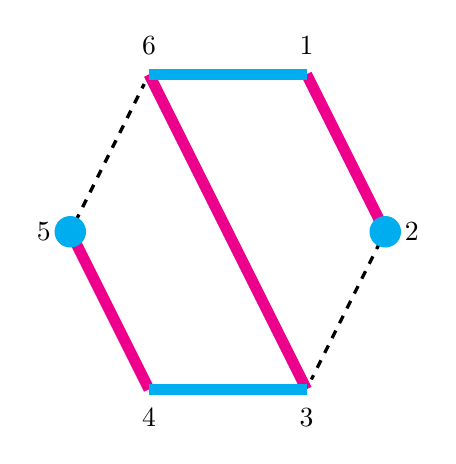
\begin{tikzpicture}[scale=1]
            \node [label = above : {$1$}] (1)
                at (4,5) {};
            \node [label = right : {$2$}] (2)
                at (5,3) {};
            \node [label = below : {$3$}] (3)
                at (4,1) {};
            \node [label = below : {$4$}] (4)
                at (2,1) {};
            \node [label = left : {$5$}]  (5)
                at (1,3) {};
            \node [label = above : {$6$}] (6)
                at (2,5) {};
            \draw [dashed][very thick]
            (1) -- (2) -- (3) -- (4)
                -- (5) -- (6) -- (1);
            \draw [color = magenta][line width = 4pt] 
                (4,5) -- (5,3);
            \draw [color = magenta][line width = 4pt] 
                (4,1) -- (2,5);
            \draw [color = magenta][line width = 4pt] 
                (2,1) -- (1,3);
            \draw [color = cyan][line width = 4pt] 
                (4,5) -- (2,5);                
            \draw [color = cyan][line width = 4pt] 
                (4,1) -- (2,1);
            \fill [color=cyan] (5,3) circle (0.2);
            \fill [color=cyan] (1,3) circle (0.2);
          \end{tikzpicture}
    \end{center}
\end{example}

\begin{example}[Counter-example : $P = \{\{1, 2\},
    \{3, 6\},\ \{4, 5\}\},
    Q = \{\{1, 6\}, \{2, 5\}, \{3, 4\}\}$]
    ~\\
    \begin{center}
        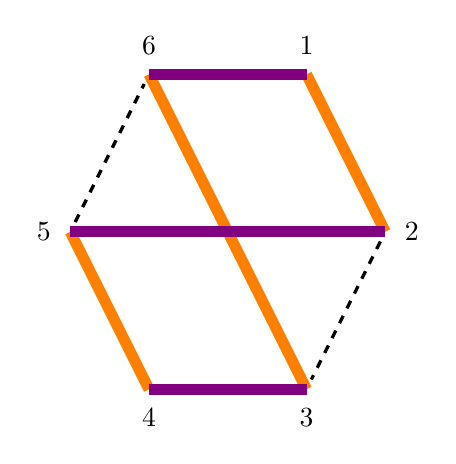
\begin{tikzpicture}[scale=1]
            \node [label = above : {$1$}] (1)
                at (4,5) {};
            \node [label = right : {$2$}] (2)
                at (5,3) {};
            \node [label = below : {$3$}] (3)
                at (4,1) {};
            \node [label = below : {$4$}] (4)
                at (2,1) {};
            \node [label = left : {$5$}]  (5)
                at (1,3) {};
            \node [label = above : {$6$}] (6)
                at (2,5) {};
            \draw [dashed][very thick]
            (1) -- (2) -- (3) -- (4)
                -- (5) -- (6) -- (1);
            \draw [color = orange][line width = 4pt] 
                (4,5) -- (5,3);
            \draw [color = orange][line width = 4pt] 
                (4,1) -- (2,5);
            \draw [color = orange][line width = 4pt] 
                (2,1) -- (1,3);
            \draw [color = violet][line width = 4pt] 
                (4,5) -- (2,5);                
            \draw [color = violet][line width = 4pt] 
                (5,3) -- (1,3);        
            \draw [color = violet][line width = 4pt] 
                (4,1) -- (2,1);

          \end{tikzpicture}
    \end{center}
\end{example}

\begin{rem}
    Note that vertices \emph{can} touch, but the edges
    of the convex hulls can \emph{not} cross.
\end{rem}

\begin{prop}
    For any non-crossing partition $P$, $P$ and $K(P)$
    are mutually non-crossing.\\
    Furthermore, $K(P)$ is a \emph{densest} partition that
    is mutually non-crossing with $P$. That is, \emph{no}
    partition $Q$ that is mutually non-crossing with $P$
    has less blocks than $K(P)$.
\end{prop}

\begin{example}[$P = \{1, 2, 6\}, \{3, 5\}, \{4\}\}$]
    $Q = \{\{1\}, \{2, 5\}, \{3, 4\}, \{6\}\}$

    \begin{center}
        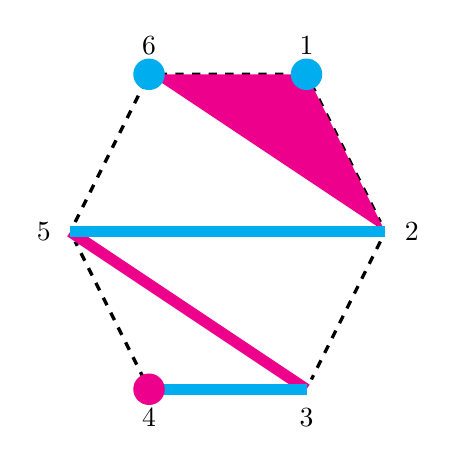
\begin{tikzpicture}[scale=1]
            \node [label = above : {$1$}] (1)
                at (4,5) {};
            \node [label = right : {$2$}] (2)
                at (5,3) {};
            \node [label = below : {$3$}] (3)
                at (4,1) {};
            \node [label = below : {$4$}] (4)
                at (2,1) {};
            \node [label = left : {$5$}]  (5)
                at (1,3) {};
            \node [label = above : {$6$}] (6)
                at (2,5) {};
            \draw [dashed][very thick]
            (1) -- (2) -- (3) -- (4)
                -- (5) -- (6) -- (1);
            \fill [color = magenta] (4,5) -- (5,3)
                -- (2,5) -- cycle;
            \draw [color = magenta][line width = 4pt] 
                (4,1) -- (1,3);
            \draw [color = cyan][line width = 4pt] 
                (4,1) -- (2,1);                
            \draw [color = cyan][line width = 4pt] 
                (5,3) -- (1,3);
            \fill [color=magenta] (2,1) circle (0.2);
            \fill [color=cyan] (4,5) circle (0.2);
            \fill [color=cyan] (2,5) circle (0.2);

          \end{tikzpicture}
    \end{center}
\end{example}

\subsection{Action of $\mathfrak{S}_n$ on partitions of 
$[n]$}

\begin{definition}[Action of $\mathfrak{S}_n$]
    The action of $\mathfrak{S}_n$ on a partition
    $P = \{B_1, \ldots, B_l\}$ of $[n]$ is defined by :\\
    \begin{itemize*}
        \item For each block $B_i = \{b_1, \ldots, b_k\}$ :
        $\sigma(Bi) =\{\sigma (b_1), \ldots, \sigma (b_k)\}$ \\
        \item When $P \in \mathcal{NC}_n$, we denote 
        $\rho = \sigma(P) =
            \{\sigma (B_1), \ldots, \sigma (B_l)\}$
    \end{itemize*}
\end{definition}

\begin{example}[$\sigma = 415362,
    P = \{\{1, 6\}, \{2, 3, 5\}, \{4\}\}$]
    ~\\
    $\sigma (P) = 
        \{\{1, 5, 6\}, \{2, 4\}, \{3\}\}$
        ~\\
    \begin{center}
        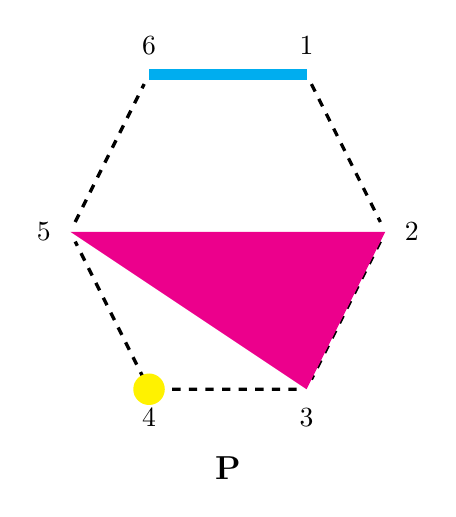
\begin{tikzpicture}[scale=1]
            \node at (3,0) {\large $\mathbf{P}$};
            \node [label = above : {$1$}] (1)
                at (4,5) {};
            \node [label = right : {$2$}] (2)
                at (5,3) {};
            \node [label = below : {$3$}] (3)
                at (4,1) {};
            \node [label = below : {$4$}] (4)
                at (2,1) {};
            \node [label = left : {$5$}]  (5)
                at (1,3) {};
            \node [label = above : {$6$}] (6)
                at (2,5) {};
            \draw [dashed][very thick]
            (1) -- (2) -- (3) -- (4)
                -- (5) -- (6) -- (1);
            \draw [color = cyan][line width = 4pt] 
                (4,5) -- (2,5);
            \fill [color = magenta] (5,3) -- (4,1)
                -- (1,3) -- cycle;
            \fill [color = yellow] (2,1) circle (0.2);
        \end{tikzpicture}
        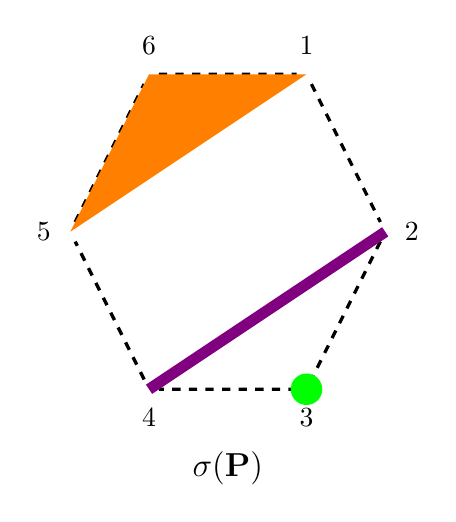
\begin{tikzpicture}[scale=1]
            \node at (3,0) {\large $\mathbf{\sigma(P)}$};
            \node [label = above : {$1$}] (1)
                at (4,5) {};
            \node [label = right : {$2$}] (2)
                at (5,3) {};
            \node [label = below : {$3$}] (3)
                at (4,1) {};
            \node [label = below : {$4$}] (4)
                at (2,1) {};
            \node [label = left : {$5$}]  (5)
                at (1,3) {};
            \node [label = above : {$6$}] (6)
                at (2,5) {};
            \draw [dashed][very thick]
            (1) -- (2) -- (3) -- (4)
                -- (5) -- (6) -- (1);
            \fill [color = orange] (4,5) -- (1,3)
                -- (2,5) -- cycle;
            \draw [color = violet][line width = 4pt] 
                (5,3) -- (2,1);
            \fill [color=green] (4,1) circle (0.2);

          \end{tikzpicture}
    \end{center}
\end{example}

\begin{rem}
    Note that $\mathcal{NC}_n$ is \emph{not} stable under
    the action of $\mathfrak{S}_n$.
    That is, even if $P$ is non-crossing, $\sigma (P)$ is 
    \emph{not} necessarily non-crossing.
\end{rem}

\begin{example}[Counter-example : $\sigma = 413562,
    P = \{\{1, 6\}, \{2, 3, 5\}, \{4\}\}$]
    $\sigma (P) = 
        \{\{1, 3, 6\}, \{2, 4\}, \{5\}\}$
        ~\\
    \begin{center}
        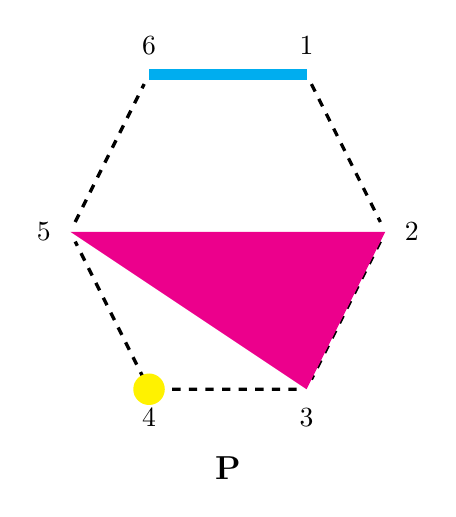
\begin{tikzpicture}[scale=1]
            \node at (3,0) {\large $\mathbf{P}$};
            \node [label = above : {$1$}] (1)
                at (4,5) {};
            \node [label = right : {$2$}] (2)
                at (5,3) {};
            \node [label = below : {$3$}] (3)
                at (4,1) {};
            \node [label = below : {$4$}] (4)
                at (2,1) {};
            \node [label = left : {$5$}]  (5)
                at (1,3) {};
            \node [label = above : {$6$}] (6)
                at (2,5) {};
            \draw [dashed][very thick]
            (1) -- (2) -- (3) -- (4)
                -- (5) -- (6) -- (1);
            \draw [color = cyan][line width = 4pt] 
                (4,5) -- (2,5);
            \fill [color = magenta] (5,3) -- (4,1)
                -- (1,3) -- cycle;
            \fill [color = yellow] (2,1) circle (0.2);
        \end{tikzpicture}
        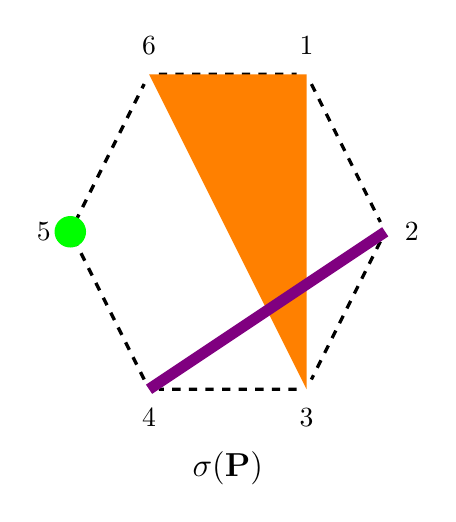
\begin{tikzpicture}[scale=1]
            \node at (3,0) {\large $\mathbf{\sigma (P)}$};
            \node [label = above : {$1$}] (1)
                at (4,5) {};
            \node [label = right : {$2$}] (2)
                at (5,3) {};
            \node [label = below : {$3$}] (3)
                at (4,1) {};
            \node [label = below : {$4$}] (4)
                at (2,1) {};
            \node [label = left : {$5$}]  (5)
                at (1,3) {};
            \node [label = above : {$6$}] (6)
                at (2,5) {};
            \draw [dashed][very thick]
            (1) -- (2) -- (3) -- (4)
                -- (5) -- (6) -- (1);
            \fill [color = orange] (4,5) -- (4,1)
                -- (2,5) -- cycle;
            \draw [color = violet][line width = 4pt] 
                (5,3) -- (2,1);
            \fill [color=green] (1,3) circle (0.2);
            
          \end{tikzpicture}
    \end{center}
\end{example}

\begin{definition}[Rotation]
    We define the \emph{rotation operator} $rot$ of
    $P \in \mathcal{NC}_n$ as $rot (P) = 
    (1\ 2\ 3\  \ldots \ n)(P) = 23 \ldots n1 (P)$.\\
    Conversely, we define $rot^{-1}$ of $P$ as
    $rot^{-1}(P) = (n\ n-1\ \ldots 3\ 2\ 1)(P) = 
    n12 \ldots n-1 (P)$.
\end{definition}

\begin{example}[$P = \{\{1, 6\}, \{2, 3, 5\}, \{4\}\}$]
    ~
    \begin{itemize}
        \item $rot (P) = \{\{1, 2\}, \{3, 4, 6\}, \{5\}\}$
        \item $rot^{-1}(P) = \{\{1, 2, 4\}, \{3\}, \{5, 6\}\}$
    \end{itemize}
    \begin{center}
    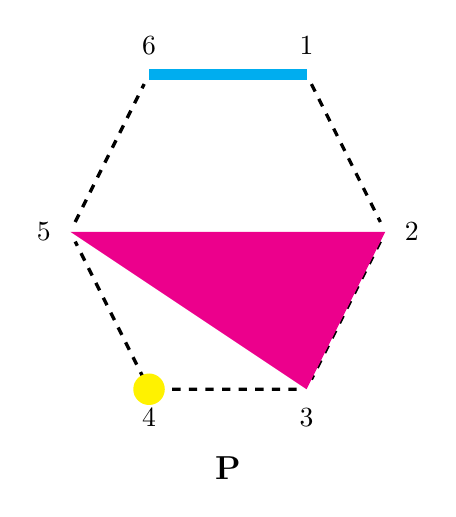
\begin{tikzpicture}[scale=1]
        \node at (3,0) {\large $\mathbf{P}$};
        \node [label = above : {$1$}] (1)
            at (4,5) {};
        \node [label = right : {$2$}] (2)
            at (5,3) {};
        \node [label = below : {$3$}] (3)
            at (4,1) {};
        \node [label = below : {$4$}] (4)
            at (2,1) {};
        \node [label = left : {$5$}]  (5)
            at (1,3) {};
        \node [label = above : {$6$}] (6)
            at (2,5) {};
        \draw [dashed][very thick]
        (1) -- (2) -- (3) -- (4)
            -- (5) -- (6) -- (1);
        \fill [color = magenta] (5,3) -- (4,1)
            -- (1,3) -- cycle;
        \draw [color = cyan][line width = 4pt] 
            (4,5) -- (2,5);
        \fill [color=yellow] (2,1) circle (0.2);
      \end{tikzpicture}
      ~\\
      ~\\

      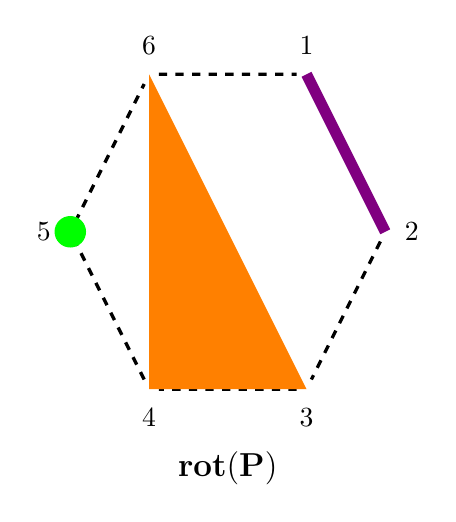
\begin{tikzpicture}[scale=1]
        \node at (3,0) {\large $\mathbf{rot(P)}$};
        \node [label = above : {$1$}] (1)
            at (4,5) {};
        \node [label = right : {$2$}] (2)
            at (5,3) {};
        \node [label = below : {$3$}] (3)
            at (4,1) {};
        \node [label = below : {$4$}] (4)
            at (2,1) {};
        \node [label = left : {$5$}]  (5)
            at (1,3) {};
        \node [label = above : {$6$}] (6)
            at (2,5) {};
        \draw [dashed][very thick]
        (1) -- (2) -- (3) -- (4)
            -- (5) -- (6) -- (1);
        \fill [color = orange] (4,1) -- (2,1)
            -- (2,5) -- cycle;
        \draw [color = violet][line width = 4pt] 
            (4,5) -- (5,3);
        \fill [color=green] (1,3) circle (0.2);    
      \end{tikzpicture}
      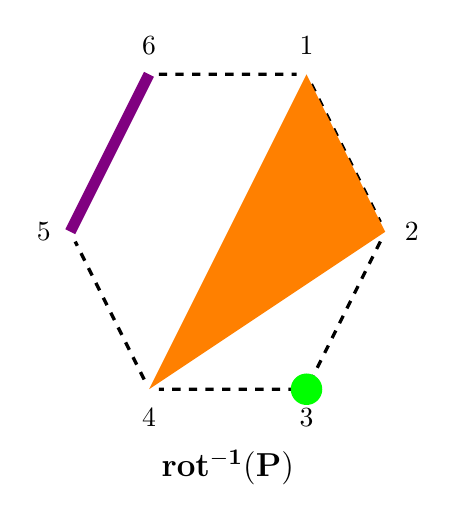
\begin{tikzpicture}[scale=1]
        \node at (3,0) {\large $\mathbf{rot^{-1}(P)}$};
        \node [label = above : {$1$}] (1)
            at (4,5) {};
        \node [label = right : {$2$}] (2)
            at (5,3) {};
        \node [label = below : {$3$}] (3)
            at (4,1) {};
        \node [label = below : {$4$}] (4)
            at (2,1) {};
        \node [label = left : {$5$}]  (5)
            at (1,3) {};
        \node [label = above : {$6$}] (6)
            at (2,5) {};
        \draw [dashed][very thick]
        (1) -- (2) -- (3) -- (4)
            -- (5) -- (6) -- (1);
        \fill [color = orange] (4,5) -- (5,3)
            -- (2,1) -- cycle;
        \draw [color = violet][line width = 4pt] 
            (1,3) -- (2,5);
        \fill [color=green] (4,1) circle (0.2);    
      \end{tikzpicture}
    \end{center}
\end{example}

\begin{rem}
    ~
    \begin{itemize}
        \item $rot (rot^{-1}(P)) = rot^{-1}(rot(P)) = P$
        \item $rot(P)$ and $rot^{-1}(P)$ are always
            non-crossing partitions.
        \item If $P \in \mathcal{NC}_n$, then $rot^n(P) =
            rot^{-n}(P) = P$.
    \end{itemize}
\end{rem}

\begin{prop}
    $K (K (P)) = rot^{-1} (P)$.
\end{prop}

\begin{example}[$P = \{\{1, 6\}, \{2, 3, 5\}, \{4\}\}$]
    ~
    \begin{center}
        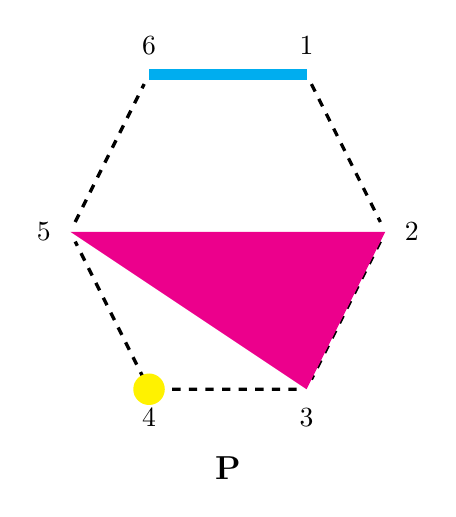
\begin{tikzpicture}[scale=1]
            \node at (3,0) {\large $\mathbf{P}$};
            \node [label = above : {$1$}] (1)
                at (4,5) {};
            \node [label = right : {$2$}] (2)
                at (5,3) {};
            \node [label = below : {$3$}] (3)
                at (4,1) {};
            \node [label = below : {$4$}] (4)
                at (2,1) {};
            \node [label = left : {$5$}]  (5)
                at (1,3) {};
            \node [label = above : {$6$}] (6)
                at (2,5) {};
            \draw [dashed][very thick]
            (1) -- (2) -- (3) -- (4)
                -- (5) -- (6) -- (1);
            \fill [color = magenta] (5,3) -- (4,1)
                -- (1,3) -- cycle;
            \draw [color = cyan][line width = 4pt] 
                (4,5) -- (2,5);
            \fill [color=yellow] (2,1) circle (0.2);
          \end{tikzpicture}
          ~\\
          ~\\
    
          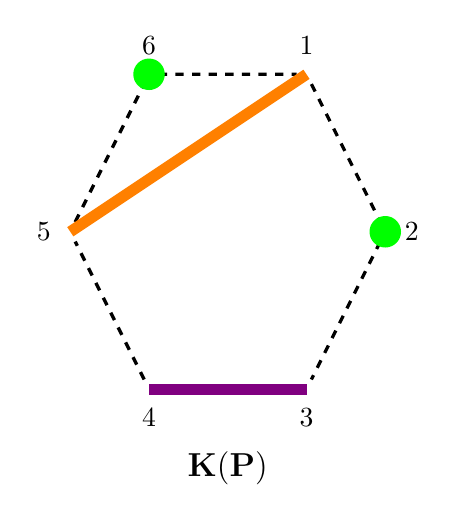
\begin{tikzpicture}[scale=1]
            \node at (3,0) {\large $\mathbf{K(P)}$};
            \node [label = above : {$1$}] (1)
                at (4,5) {};
            \node [label = right : {$2$}] (2)
                at (5,3) {};
            \node [label = below : {$3$}] (3)
                at (4,1) {};
            \node [label = below : {$4$}] (4)
                at (2,1) {};
            \node [label = left : {$5$}]  (5)
                at (1,3) {};
            \node [label = above : {$6$}] (6)
                at (2,5) {};
            \draw [dashed][very thick]
            (1) -- (2) -- (3) -- (4)
                -- (5) -- (6) -- (1);
            \draw [color = orange][line width = 4pt] 
                (4,5) -- (1,3);            
            \draw [color = violet][line width = 4pt] 
                (4,1) -- (2,1);
            \fill [color=green] (5,3) circle (0.2); 
            \fill [color=green] (2,5) circle (0.2);   
          \end{tikzpicture}
          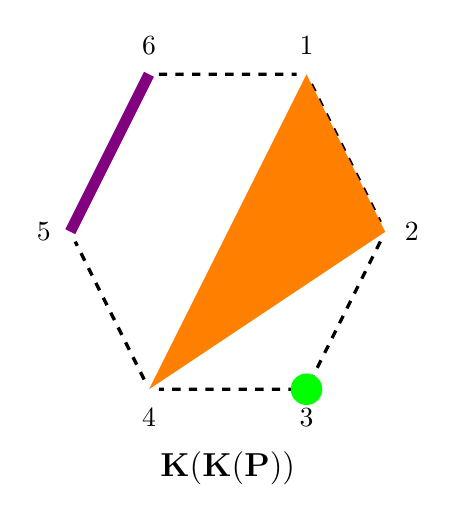
\begin{tikzpicture}[scale=1]
            \node at (3,0) {\large $\mathbf{K(K(P))}$};
            \node [label = above : {$1$}] (1)
                at (4,5) {};
            \node [label = right : {$2$}] (2)
                at (5,3) {};
            \node [label = below : {$3$}] (3)
                at (4,1) {};
            \node [label = below : {$4$}] (4)
                at (2,1) {};
            \node [label = left : {$5$}]  (5)
                at (1,3) {};
            \node [label = above : {$6$}] (6)
                at (2,5) {};
            \draw [dashed][very thick]
            (1) -- (2) -- (3) -- (4)
                -- (5) -- (6) -- (1);
            \fill [color = orange] (4,5) -- (5,3)
                -- (2,1) -- cycle;
            \draw [color = violet][line width = 4pt] 
                (1,3) -- (2,5);
            \fill [color=green] (4,1) circle (0.2);    
          \end{tikzpicture}
        \end{center}
\end{example}

\section{Non-crossing 2-partitions}

\begin{definition}[Non-crossing 2-partition]
    A \emph{non-crossing 2-partition} of a \emph{totally
    ordered} set $E$ is a pair $(P, \sigma)$
    where :\\
    \begin{itemize*}
        \item $P$ is a non-crossing partition of $E$\\
        \item $\sigma$ is a permutation of the elements of $E$\\
        \item For each \emph{sorted} block
            $B_i = \{b_1, \ldots, b_k\} \in P$, we have
            $\sigma (b_i) < \ldots < \sigma (b_k)$\\\\
    \end{itemize*}
    We denote by $\mathcal{NC}^2_n$ the set of non-crossing
    2-partitions of $[n]$.
    $$\mathcal{NC}^2 = \bigcup_{n > 0}{\mathcal{NC}^2_n}$$.
\end{definition}

\begin{example}[$\mathcal{NC}^2_6$]
    \begin{itemize*}
            \subitem $P = \{\{1, 6\}, \{2, 3, 5\}, \{4\}\}$
            \subitem $\sigma = 413265$ \\
            \subitem $\hspace{36mm} \rho = \{\{1, 3, 6\}, \{2\}, \{4, 5\}\}$
    \end{itemize*}    
\end{example}

\begin{theorem}
    Let $nc^2_n$ be the cardinal of $\mathcal{NC}^2_n$.
    We have $$nc^2_n = (n + 1)^{n-1}$$
\end{theorem}

\begin{example}[$n = 1, 2, 3$]
    ~\\
    \begin{itemize}
            \item $n = 1$ \  $:$ \  $nc^2_1 = 1$
            \subitem $\{\{1\}\}$ \hspace{1cm} $1$
                \hspace{1cm} $\rho = P$
            \item $n = 2$ \  $:$ \  $nc^2_2 = 3$
            \subitem $\{\{1\}, \{2\}\}$ \hspace{1cm} $12$
                \hspace{1cm} $\rho = P$
            \subitem $\{\{1\}, \{2\}\}$ \hspace{1cm} $21$
                \hspace{1cm} $\rho = P$
            \subitem $\{\{1, 2\}\}$ \hspace{14mm} $12$
                \hspace{1cm} $\rho = P$
            \item $n = 3$ \  $:$ \  $nc^2_3 = 16$
            \subitem $\{\{1\}, \{2\}, \{3\}\}$ \hspace{1cm}
                $123$ \hspace{1cm} $\rho = P$
            \subitem $\{\{1\}, \{2\}, \{3\}\}$ \hspace{1cm}
                $132$ \hspace{1cm} $\rho = P$
            \subitem $\{\{1\}, \{2\}, \{3\}\}$ \hspace{1cm}
                $213$ \hspace{1cm} $\rho = P$
            \subitem $\{\{1\}, \{2\}, \{3\}\}$ \hspace{1cm}
                $231$ \hspace{1cm} $\rho = P$
            \subitem $\{\{1\}, \{2\}, \{3\}\}$ \hspace{1cm}
                $312$ \hspace{1cm} $\rho = P$
            \subitem $\{\{1\}, \{2\}, \{3\}\}$ \hspace{1cm}
                $321$ \hspace{1cm} $\rho = P$       
            \subitem $\{\{1, 2\}, \{3\}\}$ \hspace{14mm}
                $123$ \hspace{1cm} $\rho = P$
            \subitem $\{\{1, 2\}, \{3\}\}$ \hspace{14mm}
                $132$ \hspace{1cm} $\rho = \{\{1, 3\}, \{2\}\}$
            \subitem $\{\{1, 2\}, \{3\}\}$ \hspace{14mm}
                $231$ \hspace{1cm} $\rho = \{\{1\}, \{2, 3\}\}$
            \subitem $\{\{1\}, \{2, 3\}\}$ \hspace{14mm}
                $123$ \hspace{1cm} $\rho = P$
            \subitem $\{\{1\}, \{2, 3\}\}$ \hspace{14mm}
                $213$ \hspace{1cm} $\rho = \{\{1, 3\}, \{2\}\}$
            \subitem $\{\{1\}, \{2, 3\}\}$ \hspace{14mm}
                $312$ \hspace{1cm} $\rho = \{\{1, 2\}, \{3\}\}$
            \subitem $\{\{1, 3\}, \{2\}\}$ \hspace{14mm}
                $123$ \hspace{1cm} $\rho = P$
            \subitem $\{\{1, 3\}, \{2\}\}$ \hspace{14mm}
                $132$ \hspace{1cm} $\rho = \{\{1, 2\}, \{3\}\}$
            \subitem $\{\{1, 3\}, \{2\}\}$ \hspace{14mm}
                $213$ \hspace{1cm} $\rho = \{\{1\}, \{2, 3\}\}$  
            \subitem $\{\{1, 2, 3\}\}$ \hspace{18mm}
                $123$ \hspace{1cm} $\rho = P$\\
    \end{itemize}
\end{example}

\begin{prop}
    This means we can create a \emph{bijection} between
    $\mathcal{PF}_n$ and $\mathcal{NC}^2_n$.
\end{prop}

\begin{proof}
    ~\\
\begin{itemize}
    \item $\mathcal{PF}_n \to \mathcal{NC}^2_n$ :
    Let $f = (a_1, \ldots, a_n) \in \mathcal{PF}_n$
    be our parking function.
    For $i \in \{1, \ldots, n\}$, we define :
        \subitem $l_i$ : the number of occurences of $i$ in $f$. 
        \subitem $im_i$ : $\{j\ |\ a_j = i\}$\\
    The corresponding non-crossing partition will
    have the following constraints :
        \subitem For each $i \in \{1, \ldots, n\}$, if $l_i > 0$,
        then there is a block $B_{[i]}$ of length
        \subitem $l_i$ with minimum element $i$.
        \subitem $\sigma (B_{[i]}) = im_i$\\
    There is a unique set partition
    $\displaystyle P = \bigcup_{i}{B}_{[i]}$ of $[n]$
    and a unique permutation $\sigma$ respecting these
    conditions such that $(P, \sigma) \in \mathcal{NC}^2_n$ :
    for each minimum $i$ in \emph{decreasing order}, add
    the $n_i$ first free elements of
    $[i+1, i+2, \ldots, n, 1, \ldots, i-1]$ to $B_i$.
    $\sigma$ is then trivially obtained by the second
    constraint. 
    \item $\mathcal{NC}^2_n \to \mathcal{PF}_n$ :
    Let $(P, \sigma)$ with $P = \{B_1, \ldots, B_l\}$ be our
    non-crossing 2-partition.
    For each block $B_i = \{b_1, \ldots, b_k\} \in P$ :
    \subitem $m_i = min (B_i) = b_1$
    \subitem $pos_i = \sigma (B_i)$
    \subitem For each $j \in pos_i$, we define $a_j = m_i$\\
    The corresponding parking function is $(a_1, \ldots, a_n)$.
\end{itemize}
\end{proof}

\begin{example}[$n = 8$]
    \begin{align*}
        &P = \{\{1, 2, 5\}, \{3, 4\}, \{6, 8\}, \{7\}\}\\
        &\sigma = 36187245\\
        &f = (3, 6, 1, 7, 6, 1, 1, 3)\\
    \end{align*}
\end{example}

\subsection{The non-crossing 2-partitions poset}

\begin{definition}[$\succ^2$]
    We say that $(P, \sigma)$ covers $(Q, \tau)$, written
    ($P, \sigma) \succ^2 (Q, \tau)$,
    if $\exists B_i, B_j \in P$ such that\\
    \begin{itemize*}
        \item $Q = P - \{B_i, B_j\} \cup \{B_i \cup B_j\}$\\
        \item $l \neq i, j \and b \in B_l \rightarrow
            \tau (b) = \sigma (b)$\\
        \item Let $B_i \cup B_j = \{b_1, \ldots, b_k\}$ :\\
            \subitem $\tau (B_i \cup B_j) = \sigma (B_i \cup B_j)$\\
            \subitem $\tau (b_1) < \ldots < \tau (b_k)$
    \end{itemize*}    
\end{definition}

\begin{example}
    ~\\
    \begin{itemize*}
        \item $P = \{\{1, 6\}, \{2, 3\}, \{4\}, \{5\}\}$\\
        \item $\sigma = 236154$\\
        \item $Q = \{\{1, 6\}, \{2, 3, 5\}, \{4\}\}$\\
        \item $\tau = 235164$\\
        \item $(P, \sigma) \succ^2 (Q, \tau)$\\
        \item $(P, \sigma) \not \succ^2 (Q, \sigma)$,
        because  $\sigma (\{2, 3, 5\}) = \{3, 6, 5\}$ is
        \emph{not} ordemagenta. 
    \end{itemize*}
\end{example}

\begin{prop}
    This covering relation defines the \emph{poset} of
    $\mathcal{NC}^2_n$.
\end{prop}

\begin{rem}
    The bottom element of this poset is 
    $(\{\{1, \ldots, n\}\}, 12 \ldots n)$, and the top
    elements are $\{(\{\{1\}, \ldots, \{n\}\}, \sigma)\ 
    |\ \sigma \in \mathfrak{S}_n\}$.
\end{rem}

\begin{example}[The poset of $\mathcal{NC}^2_3$]
    ~\\
    To shorten labels, we represent
    $(\{\{1, 3\}, \{2\}\}, 213)$ by \\
    \begin{center}
        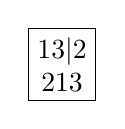
\begin{tikzpicture}
            \node (0) at (0,0) [align = center]
            [rectangle, draw]{$13|2$\\$213$};
        \end{tikzpicture}
    \end{center}

    \begin{center}
        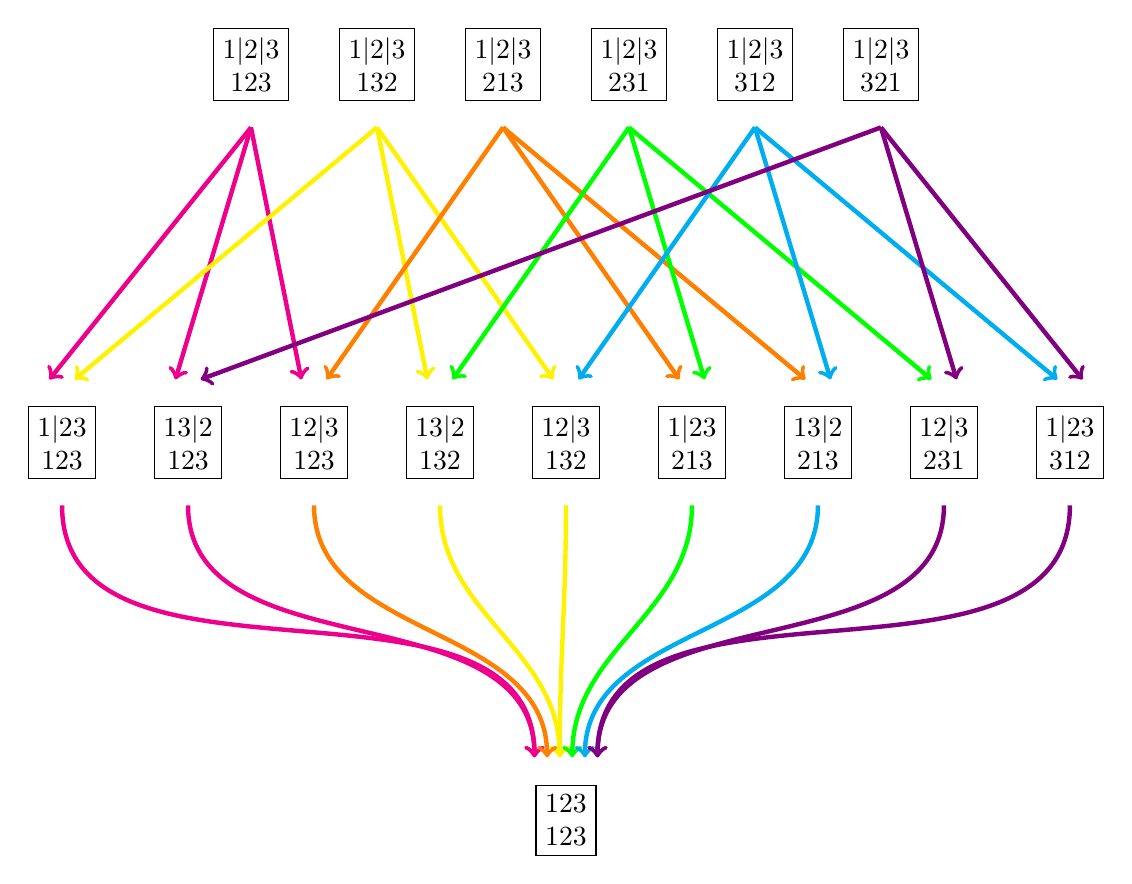
\begin{tikzpicture}[scale = 0.8]
            \node (0)  at (0,0) [align = center]
            [rectangle, draw]
                {$123$\\$123$};
            \node (1)  at (-8,6)[align = center]
            [rectangle, draw]
                {$1|23$\\$123$};
            \node (2)  at (-6,6) [align = center]
            [rectangle, draw]
                {$13|2$\\$123$};
            \node (3)  at (-4,6) [align = center]
            [rectangle, draw]
                {$12|3$\\$123$};
            \node (4)  at (-2,6) [align = center]
            [rectangle, draw]
                {$13|2$\\$132$};
            \node (5)  at (0,6) [align = center]
            [rectangle, draw]
                {$12|3$\\$132$};
            \node (6)  at (2,6) [align = center]
            [rectangle, draw]
                {$1|23$\\$213$};
            \node (7)  at (4,6) [align = center]
            [rectangle, draw]
                {$13|2$\\$213$};
            \node (8)  at (6,6) [align = center]
            [rectangle, draw]
                {$12|3$\\$231$};
            \node (9)  at (8,6) [align = center]
            [rectangle, draw]
                {$1|23$\\$312$};
            \node (10) at (-5,12) [align = center]
            [rectangle, draw]
                {$1|2|3$\\$123$};
            \node (11) at (-3,12) [align = center]
            [rectangle, draw]
                {$1|2|3$\\$132$};
            \node (12) at (-1,12) [align = center]
            [rectangle, draw]
                {$1|2|3$\\$213$};
            \node (13) at (1,12) [align = center]
            [rectangle, draw]
                {$1|2|3$\\$231$};
            \node (14) at (3,12) [align = center]
            [rectangle, draw]
                {$1|2|3$\\$312$};
            \node (15) at (5,12) [align = center]
            [rectangle, draw]
                {$1|2|3$\\$321$};
        
            \draw [->][color=magenta, ultra thick]
                (-5,11) to (-8.2,7);
            \draw [->][color=magenta, ultra thick]
                (-5,11) to (-6.2, 7); 
            \draw [->][color=magenta, ultra thick]
                (-5,11) to (-4.2,7);
            \draw [->][out=-90,in=90, ultra thick] 
                [color=magenta](-8,5) to (-0.5,1);
            \draw [->][out=-90,in=90, ultra thick] 
                [color=magenta](-6,5) to (-0.5,1);
        
            \draw [->][color=yellow, ultra thick]
                (-3,11) to (-7.8,7);
            \draw [->][color=yellow, ultra thick]
                (-3,11) to (-2.2,7);
            \draw [->][color=yellow, ultra thick]
                (-3,11) to (-0.2, 7);
            \draw [->][out=-90,in=90, ultra thick] 
                [color=yellow](-2,5) to (-0.1,1);
            \draw [->][out=-90,in=90, ultra thick] 
                [color=yellow](0,5) to (-0.1,1);
            
            \draw [->][color=orange, ultra thick]
                (-1,11) to (1.8,7);
            \draw [->][color=orange, ultra thick]
                (-1,11) to (3.8,7);
            \draw [->][color=orange, ultra thick]
                (-1,11) to (-3.8,7);
            \draw [->][out=-90,in=90, ultra thick] 
                [color=orange](-4,5) to (-0.3,1);
        
            \draw [->][color=green, ultra thick]
                (1,11) to (2.2,7);
            \draw [->][color=green, ultra thick]
                (1,11) to (-1.8,7);
            \draw [->][color=green, ultra thick]
                (1,11) to (5.8,7);
            \draw [->][out=-90,in=90, ultra thick] 
                [color=green](2,5) to (0.1,1);
        
            \draw [->][color=cyan, ultra thick]
                (3,11) to (7.8,7);
            \draw [->][color=cyan, ultra thick]
                (3,11) to (4.2,7);
            \draw [->][color=cyan, ultra thick]
                (3,11) to (0.2,7);
            \draw [->][out=-90,in=90, ultra thick] 
                [color=cyan](4,5) to (0.3,1);
        
            \draw [->][color=violet, ultra thick]
                (5,11) to (8.2,7);
            \draw [->][color=violet, ultra thick]
                (5,11) to (-5.8,7);
            \draw [->][color=violet, ultra thick]
                (5,11) to (6.2,7);
            \draw [->][out=-90,in=90, ultra thick] 
                [color=violet](6,5) to (0.5,1);
            \draw [->][out=-90,in=90, ultra thick] 
                [color=violet](8,5) to (0.5,1);
            
        \end{tikzpicture}
        ~\\
        There are $4^2 = 16$ elements in this poset.
    \end{center}
\end{example}

\subsection{The parking functions poset}

\begin{definition}[Rank]
    Given $f = (a_1, \ldots, a_n) \in \mathcal{PF}_n$, let
    $$b_i =
    \begin{cases}
        1 \text{ if } \exists j\ |\ a_j = i\\
        0 \text{ otherwise}
    \end{cases} $$
    We define the \emph{rank} of $f$, noted $rk(f)$, as
    $$\sum_{1 \leq i \leq n}{b_i}$$
\end{definition}

\begin{example}
    \begin{align*}
        &rk((1, 5, 4, 2, 3, 3, 1)) = 5\\
        &rk((4, 7, 1, 1, 3, 2 ,2, 8)) = 6\\
    \end{align*}
\end{example}

\begin{definition}[$\succ_{pf}$]
    Since $\mathcal{PF}_n$ and $\mathcal{NC}^2_n$ are
    in bijection, we can define a \emph{covering relation}
    $\succ_{pf}$ for $\mathcal{PF}_n$ as follows :\\
    $f \in \mathcal{PF}_n \succ_{pf} g \in \mathcal{PF}_n$
    if and only if :    
    \begin{itemize}
        \item $(P,\sigma)$ is the non-crossing 2-partition
        associated to $f$
        \item $(Q, \tau)$ is the non-crossing 2-partition
        associated to $g$
        \item $(P, \sigma) \succ^2 (Q, \tau)$
    \end{itemize}
\end{definition}

\begin{example}
    ~\\
    \begin{itemize*}
        \item $P = \{\{1, 6\}, \{2, 3\}, \{4\}, \{5\}\}$\\
        \item $\sigma = 236154$\\
        \item $Q = \{\{1, 6\}, \{2, 3, 5\}, \{4\}\}$\\
        \item $\tau = 235164$\\
        \item $f = (4, 1, 2, 1, 5, 2) \succ_{pf}
            g = (4, 1, 2, 1, 2, 2)$\\
    \end{itemize*}
\end{example}

\begin{rem}
    If $f \succ_{pf} g$, then $rk(f) = rk(g) + 1$, and
    there exists $i$ and $j$ such that :
    \begin{itemize}
        \item $i < j$
        \item There is at least $1$ occurence of $i$ in $f$
        \item There is at least $1$ occurence of $j$ in $f$
        $$b_k =
            \begin{cases}
                i \text{ if } a_k = j\\
                a_k \text{ otherwise}\\
            \end{cases}$$
    \end{itemize}
\end{rem}

\begin{prop}
    This covering relation defines the \emph{poset}
    of $\mathcal{PF}_n$.
\end{prop}

\begin{rem}
    The bottom element of this poset is
    $(\underbrace{1, \ldots, 1}_{n})$,
    and the top elements are the \emph{permutations} of
    $\{1, \ldots, n\}$.
\end{rem}

\begin{example}[The poset of $\mathcal{PF}_3$]
    ~\\
    \begin{center}
        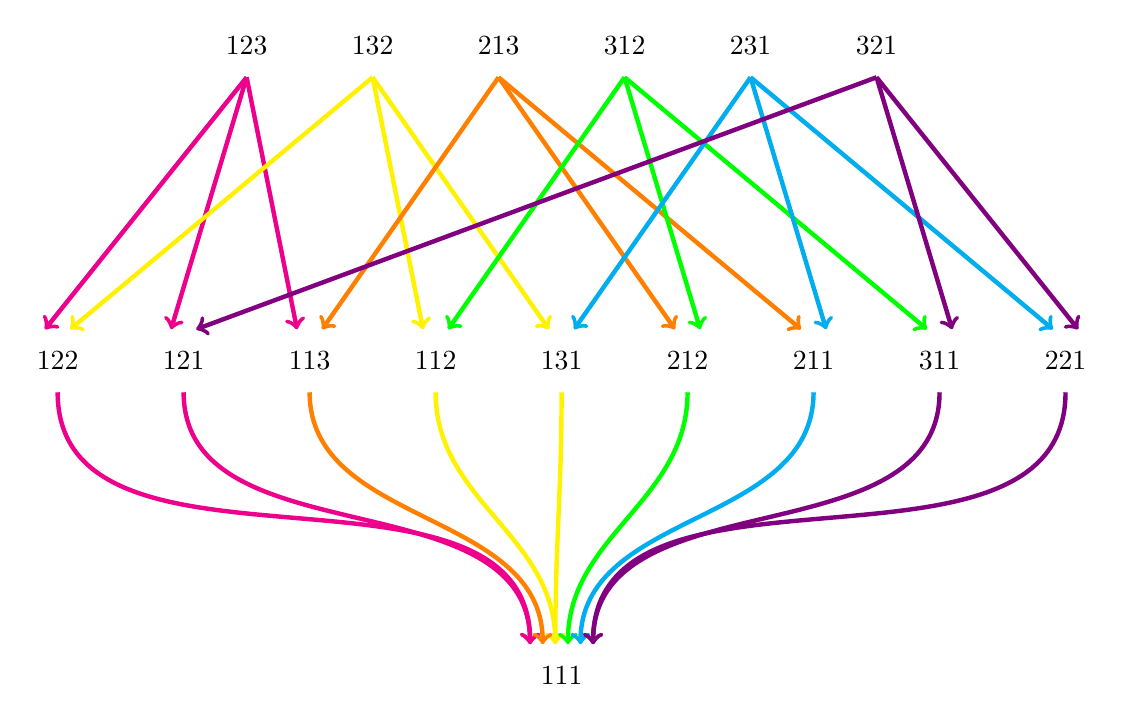
\begin{tikzpicture}[scale = 0.8]
            \node (0)  at (0,0)   {$111$};
            \node (1)  at (-8,5)  {$122$};
            \node (2)  at (-6,5)  {$121$};
            \node (3)  at (-4,5)  {$113$};
            \node (4)  at (-2,5)  {$112$};
            \node (5)  at (0,5)   {$131$};
            \node (6)  at (2,5)   {$212$};
            \node (7)  at (4,5)   {$211$};
            \node (8)  at (6,5)   {$311$};
            \node (9)  at (8,5)   {$221$};
            \node (10) at (-5,10) {$123$};
            \node (11) at (-3,10) {$132$};
            \node (12) at (-1,10) {$213$};
            \node (13) at (1,10)  {$312$};
            \node (14) at (3,10)  {$231$};
            \node (15) at (5,10)  {$321$};
        
            \draw [->][color=magenta, ultra thick]
                (-5,9.5) to (-8.2,5.5);
            \draw [->][color=magenta, ultra thick]
                (-5,9.5) to (-6.2,5.5); 
            \draw [->][color=magenta, ultra thick]
                (-5,9.5) to (-4.2,5.5);
            \draw [->][out=-90,in=90, ultra thick] 
                [color=magenta](-8,4.5) to (-0.5,0.5);
            \draw [->][out=-90,in=90, ultra thick] 
                [color=magenta](-6,4.5) to (-0.5,0.5);
        
            \draw [->][color=yellow, ultra thick]
                (-3,9.5) to (-7.8,5.5);
            \draw [->][color=yellow, ultra thick]
                (-3,9.5) to (-2.2,5.5);
            \draw [->][color=yellow, ultra thick]
                (-3,9.5) to (-0.2,5.5);
            \draw [->][out=-90,in=90, ultra thick] 
                [color=yellow](-2,4.5) to (-0.1,0.5);
            \draw [->][out=-90,in=90, ultra thick] 
                [color=yellow](0,4.5) to (-0.1,0.5);
            
            \draw [->][color=orange, ultra thick]
                (-1,9.5) to (1.8,5.5);
            \draw [->][color=orange, ultra thick]
                (-1,9.5) to (3.8,5.5);
            \draw [->][color=orange, ultra thick]
                (-1,9.5) to (-3.8,5.5);
            \draw [->][out=-90,in=90, ultra thick] 
                [color=orange](-4,4.5) to (-0.3,0.5);
        
            \draw [->][color=green, ultra thick]
                (1,9.5) to (2.2,5.5);
            \draw [->][color=green, ultra thick]
                (1,9.5) to (-1.8,5.5);
            \draw [->][color=green, ultra thick]
                (1,9.5) to (5.8,5.5);
            \draw [->][out=-90,in=90, ultra thick] 
                [color=green](2,4.5) to (0.1,0.5);
        
            \draw [->][color=cyan, ultra thick]
                (3,9.5) to (7.8,5.5);
            \draw [->][color=cyan, ultra thick]
                (3,9.5) to (4.2,5.5);
            \draw [->][color=cyan, ultra thick]
                (3,9.5) to (0.2,5.5);
            \draw [->][out=-90,in=90, ultra thick] 
                [color=cyan](4,4.5) to (0.3,0.5);
        
            \draw [->][color=violet, ultra thick]
                (5,9.5) to (8.2,5.5);
            \draw [->][color=violet, ultra thick]
                (5,9.5) to (-5.8,5.5);
            \draw [->][color=violet, ultra thick]
                (5,9.5) to (6.2,5.5);
            \draw [->][out=-90,in=90, ultra thick] 
                [color=violet](6,4.5) to (0.5,0.5);
            \draw [->][out=-90,in=90, ultra thick] 
                [color=violet](8,4.5) to (0.5,0.5);
            
        \end{tikzpicture}
    \end{center}
\end{example}

\section{A direct poset linked to Dyck paths}

\subsection{Dyck Paths}

\begin{notation}
    We denote the number of occurences of a symbol $s$ in
    a word $w$ by $|w|_s$.
\end{notation}

\begin{definition}[Dyck path]
    A \emph{Dyck word} is a word $w \in \{0,1\}^*$ such
    that :
    \begin{itemize}
        \item for each \emph{suffix} $w'$ of $w$,
            $|w'|_1 \geqslant |w'|_0$.
        \item $|w|_0 = |w|_1$.
    \end{itemize}
    A Dyck word of length $2n$ can be represented as a 
    \emph{path} from $(0,0)$ to $(n,n)$ that stays over
    $x = y$, called a \emph{Dyck path} :
    \begin{itemize}
        \item Each $1$ corresponds to a \emph{North step}
        $\uparrow$. 
        \item Each $0$ corresponds to an \emph{East step}
        $\rightarrow$.
    \end{itemize}
    We denote by $\mathcal{D}_n$ the set of Dyck words of
    length $2n$.
\end{definition}

\begin{example}[$n = 5$]
    ~\\
    \begin{align*}
        &w_1 = 1011000110 \text{ is \emph{not} a Dyck word,
        because } |1011000|_0 > |1011000|_1.\\
        &w_2 = 1011010101 \text{ is \emph{not} a Dyck word,
        because } |w_2|_0 \neq |w_2|_1.\\
        &w_3 = 1011010100 \text{ \emph{is} a Dyck word : }\\
    \end{align*}
    \begin{center}
        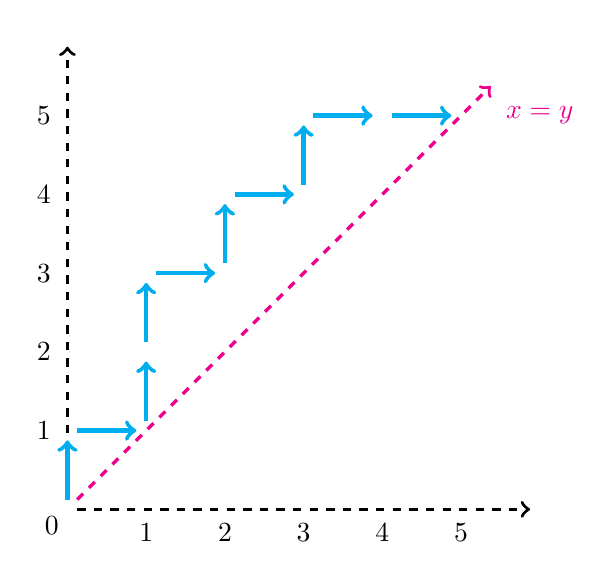
\begin{tikzpicture}[scale=1]
            \node (a) at (0, 0) {};
            \node (b) at (0, 6) {};
            \node (c) at (6, 0) {};
            \node (d) at (5.5, 5.5) {};
            \node (e) at (6, 5) [color = magenta]
                {$x = y$}; 
            \draw [dashed, very thick, ->] (a) to (b);
            \draw [dashed, very thick, ->] (a) to (c);
            \draw [dashed, very thick, ->]
                [color = magenta] (a) to (d);

            \node (1)  at (0,0)   {};
            \node (2)  at (0,1)   {};
            \node (3)  at (1,1)   {};
            \node (4)  at (1,2)   {};
            \node (5)  at (1,3)   {};
            \node (6)  at (2,3)   {};
            \node (7)  at (2,4)   {};
            \node (8)  at (3,4)   {};
            \node (9)  at (3,5)   {};
            \node (10) at (4,5)   {};
            \node (11) at (5,5)   {};
            \draw [->, ultra thick, color = cyan]
                (1)  to (2);
            \draw [->, ultra thick, color = cyan] 
                (2)  to (3);
            \draw [->, ultra thick, color = cyan]
                (3)  to (4);
            \draw [->, ultra thick, color = cyan]
                (4)  to (5);
            \draw [->, ultra thick, color = cyan]
                (5)  to (6);
            \draw [->, ultra thick, color = cyan]
                (6)  to (7);
            \draw [->, ultra thick, color = cyan]
                (7)  to (8);
            \draw [->, ultra thick, color = cyan]
                (8)  to (9);
            \draw [->, ultra thick, color = cyan]
                (9)  to (10);
            \draw [->, ultra thick, color = cyan]
                (10) to (11);

            \node at (-0.2, -0.2) {$0$};
            \node at (-0.3, 1)    {$1$};
            \node at (1, -0.3)    {$1$};
            \node at (-0.3, 2)    {$2$};
            \node at (2, -0.3)    {$2$};
            \node at (-0.3, 3)    {$3$};
            \node at (3, -0.3)    {$3$};
            \node at (-0.3, 4)    {$4$};
            \node at (4, -0.3)    {$4$};
            \node at (-0.3, 5)    {$5$};
            \node at (5, -0.3)    {$5$};

        \end{tikzpicture}
    \end{center}
\end{example}

\begin{theorem}
    Let $d_n$ be the cardinal of $\mathcal{D}_n$.
    We have $$d_n = \frac{1}{n + 1} \binom {2n}{n}$$
    which is the $n^{th}$ Catalan number.
\end{theorem}

\begin{example}[$n = 3$]
    $d_n = 5$.
    \begin{center}
        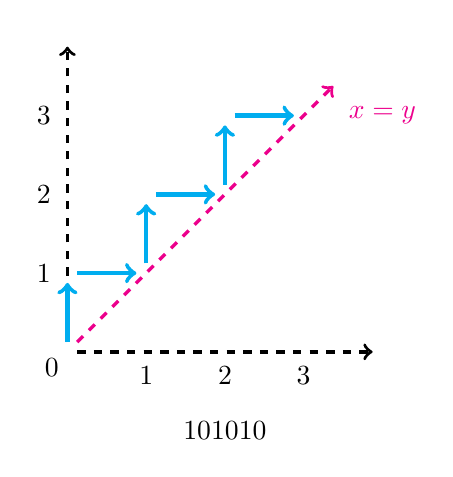
\begin{tikzpicture}[scale = 1]
            \node (a) at (0, 0) {};
            \node (b) at (0, 4) {};
            \node (c) at (4, 0) {};
            \node (d) at (3.5, 3.5) {};
            \node (e) at (4, 3) [color = magenta]
                {$x = y$}; 
            \draw [dashed, very thick, ->] (a) to (b);
            \draw [dashed, very thick, ->] (a) to (c);
            \draw [dashed, very thick, ->]
                [color = magenta] (a) to (d);

            \node (1)  at (0,0)   {};
            \node (2)  at (0,1)   {};
            \node (3)  at (1,1)   {};
            \node (4)  at (1,2)   {};
            \node (5)  at (2,2)   {};
            \node (6)  at (2,3)   {};
            \node (7)  at (3,3)   {};
            \draw [->, ultra thick, color = cyan]
                (1)  to (2);
            \draw [->, ultra thick, color = cyan] 
                (2)  to (3);
            \draw [->, ultra thick, color = cyan]
                (3)  to (4);
            \draw [->, ultra thick, color = cyan]
                (4)  to (5);
            \draw [->, ultra thick, color = cyan]
                (5)  to (6);
            \draw [->, ultra thick, color = cyan]
                (6)  to (7);

            \node at (-0.2, -0.2) {$0$};
            \node at (-0.3, 1)    {$1$};
            \node at (1, -0.3)    {$1$};
            \node at (-0.3, 2)    {$2$};
            \node at (2, -0.3)    {$2$};
            \node at (-0.3, 3)    {$3$};
            \node at (3, -0.3)    {$3$};
            \node at (2, -1)      {$101010$};

        \end{tikzpicture}
        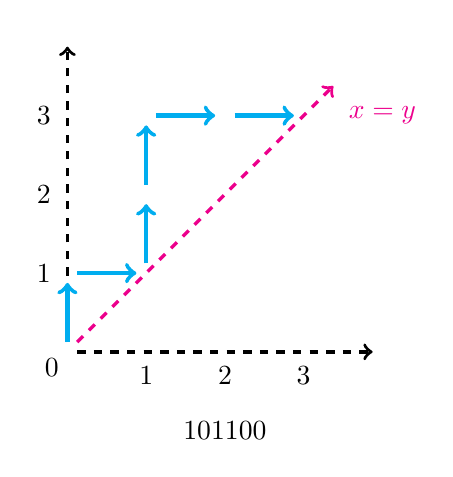
\begin{tikzpicture}[scale = 1]
            \node (a) at (0, 0) {};
            \node (b) at (0, 4) {};
            \node (c) at (4, 0) {};
            \node (d) at (3.5, 3.5) {};
            \node (e) at (4, 3) [color = magenta]
                {$x = y$}; 
            \draw [dashed, very thick, ->] (a) to (b);
            \draw [dashed, very thick, ->] (a) to (c);
            \draw [dashed, very thick, ->]
                [color = magenta] (a) to (d);

            \node (1)  at (0,0)   {};
            \node (2)  at (0,1)   {};
            \node (3)  at (1,1)   {};
            \node (4)  at (1,2)   {};
            \node (5)  at (1,3)   {};
            \node (6)  at (2,3)   {};
            \node (7)  at (3,3)   {};
            \draw [->, ultra thick, color = cyan]
                (1)  to (2);
            \draw [->, ultra thick, color = cyan] 
                (2)  to (3);
            \draw [->, ultra thick, color = cyan]
                (3)  to (4);
            \draw [->, ultra thick, color = cyan]
                (4)  to (5);
            \draw [->, ultra thick, color = cyan]
                (5)  to (6);
            \draw [->, ultra thick, color = cyan]
                (6)  to (7);

            \node at (-0.2, -0.2) {$0$};
            \node at (-0.3, 1)    {$1$};
            \node at (1, -0.3)    {$1$};
            \node at (-0.3, 2)    {$2$};
            \node at (2, -0.3)    {$2$};
            \node at (-0.3, 3)    {$3$};
            \node at (3, -0.3)    {$3$};
            \node at (2, -1)      {$101100$};

        \end{tikzpicture}        
        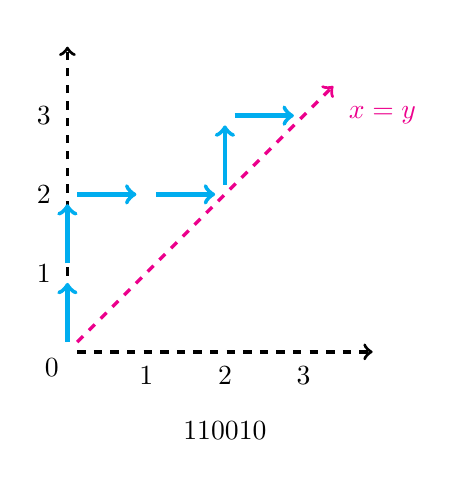
\begin{tikzpicture}[scale = 1]
            \node (a) at (0, 0) {};
            \node (b) at (0, 4) {};
            \node (c) at (4, 0) {};
            \node (d) at (3.5, 3.5) {};
            \node (e) at (4, 3) [color = magenta]
                {$x = y$}; 
            \draw [dashed, very thick, ->] (a) to (b);
            \draw [dashed, very thick, ->] (a) to (c);
            \draw [dashed, very thick, ->]
                [color = magenta] (a) to (d);

            \node (1)  at (0,0)   {};
            \node (2)  at (0,1)   {};
            \node (3)  at (0,2)   {};
            \node (4)  at (1,2)   {};
            \node (5)  at (2,2)   {};
            \node (6)  at (2,3)   {};
            \node (7)  at (3,3)   {};
            \draw [->, ultra thick, color = cyan]
                (1)  to (2);
            \draw [->, ultra thick, color = cyan] 
                (2)  to (3);
            \draw [->, ultra thick, color = cyan]
                (3)  to (4);
            \draw [->, ultra thick, color = cyan]
                (4)  to (5);
            \draw [->, ultra thick, color = cyan]
                (5)  to (6);
            \draw [->, ultra thick, color = cyan]
                (6)  to (7);

            \node at (-0.2, -0.2) {$0$};
            \node at (-0.3, 1)    {$1$};
            \node at (1, -0.3)    {$1$};
            \node at (-0.3, 2)    {$2$};
            \node at (2, -0.3)    {$2$};
            \node at (-0.3, 3)    {$3$};
            \node at (3, -0.3)    {$3$};
            \node at (2, -1)      {$110010$};
        \end{tikzpicture}
        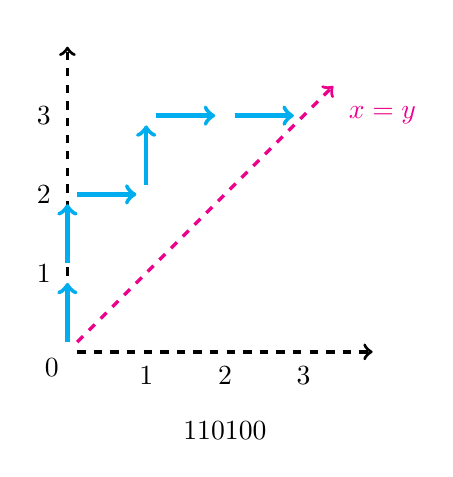
\begin{tikzpicture}[scale = 1]
            \node (a) at (0, 0) {};
            \node (b) at (0, 4) {};
            \node (c) at (4, 0) {};
            \node (d) at (3.5, 3.5) {};
            \node (e) at (4, 3) [color = magenta]
                {$x = y$}; 
            \draw [dashed, very thick, ->] (a) to (b);
            \draw [dashed, very thick, ->] (a) to (c);
            \draw [dashed, very thick, ->]
                [color = magenta] (a) to (d);

            \node (1)  at (0,0)   {};
            \node (2)  at (0,1)   {};
            \node (3)  at (0,2)   {};
            \node (4)  at (1,2)   {};
            \node (5)  at (1,3)   {};
            \node (6)  at (2,3)   {};
            \node (7)  at (3,3)   {};
            \draw [->, ultra thick, color = cyan]
                (1)  to (2);
            \draw [->, ultra thick, color = cyan] 
                (2)  to (3);
            \draw [->, ultra thick, color = cyan]
                (3)  to (4);
            \draw [->, ultra thick, color = cyan]
                (4)  to (5);
            \draw [->, ultra thick, color = cyan]
                (5)  to (6);
            \draw [->, ultra thick, color = cyan]
                (6)  to (7);

            \node at (-0.2, -0.2) {$0$};
            \node at (-0.3, 1)    {$1$};
            \node at (1, -0.3)    {$1$};
            \node at (-0.3, 2)    {$2$};
            \node at (2, -0.3)    {$2$};
            \node at (-0.3, 3)    {$3$};
            \node at (3, -0.3)    {$3$};
            \node at (2, -1)      {$110100$};
        \end{tikzpicture}
        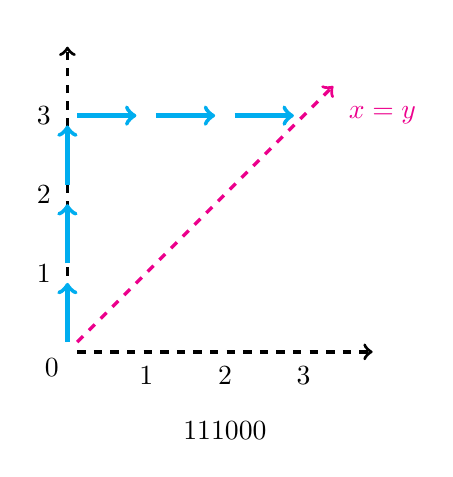
\begin{tikzpicture}[scale = 1]
            \node (a) at (0, 0) {};
            \node (b) at (0, 4) {};
            \node (c) at (4, 0) {};
            \node (d) at (3.5, 3.5) {};
            \node (e) at (4, 3) [color = magenta]
                {$x = y$}; 
            \draw [dashed, very thick, ->] (a) to (b);
            \draw [dashed, very thick, ->] (a) to (c);
            \draw [dashed, very thick, ->]
                [color = magenta] (a) to (d);

            \node (1)  at (0,0)   {};
            \node (2)  at (0,1)   {};
            \node (3)  at (0,2)   {};
            \node (4)  at (0,3)   {};
            \node (5)  at (1,3)   {};
            \node (6)  at (2,3)   {};
            \node (7)  at (3,3)   {};
            \draw [->, ultra thick, color = cyan]
                (1)  to (2);
            \draw [->, ultra thick, color = cyan] 
                (2)  to (3);
            \draw [->, ultra thick, color = cyan]
                (3)  to (4);
            \draw [->, ultra thick, color = cyan]
                (4)  to (5);
            \draw [->, ultra thick, color = cyan]
                (5)  to (6);
            \draw [->, ultra thick, color = cyan]
                (6)  to (7);

            \node at (-0.2, -0.2) {$0$};
            \node at (-0.3, 1)    {$1$};
            \node at (1, -0.3)    {$1$};
            \node at (-0.3, 2)    {$2$};
            \node at (2, -0.3)    {$2$};
            \node at (-0.3, 3)    {$3$};
            \node at (3, -0.3)    {$3$};
            \node at (2, -1)      {$111000$};
        \end{tikzpicture}
    \end{center}
\end{example}

\begin{prop}
    This means we can create a \emph{bijection} between
    $\mathcal{PF'}_n$ and $\mathcal{D}_n$.
\end{prop}

\begin{proof}
    ~\
\begin{itemize}
    \item $\mathcal{PF'}_n \to \mathcal{D}_n$ :
    Let $f = (a_1, \ldots, a_n) \in \mathcal{PF'}_n$
    be our primitive parking function.
    For $i \in \{1, \ldots, n\}$, we define $l_i$ the
    number of occurences of $i$ in $f$.\\
    The corresponding Dyck word will be
    $\underbrace{1 \cdots 1}_{l_1}0
     \underbrace{1 \cdots 1}_{l_2}0 \cdots
     \underbrace{1 \cdots 1}_{l_n}0$.
    
    \item $\mathcal{D}_n \to \mathcal{PF'}_n$ :
    Let $w$ be our Dyck word, and consider its path
    representation. We define $s_i$ to be the distance
    between the segment from $(0, i - 1)$ to $(0, i)$
    and the $i^{th}$ North step. Then, let $a_i = s_i + 1$.\\
    The corresponding primitive parking function is 
    $(a_1, \ldots, a_n)$.
\end{itemize}
\end{proof}

\begin{example}[$n = 6, \mathcal{PF'}_n \to \mathcal{D}_n$]
    ~\
    \begin{itemize}
        \item $f = (1, 1, 2, 4, 5, 5)$
            \subitem $l_1 = 2$
            \hspace{2cm} $l_2 = 1$
            \hspace{2cm} $l_3 = 0$
            \subitem $l_4 = 1$
            \hspace{2cm} $l_5 = 2$
            \hspace{2cm} $l_6 = 0$
        \item $w = (110100101100)$
    \end{itemize}

    \begin{center}
        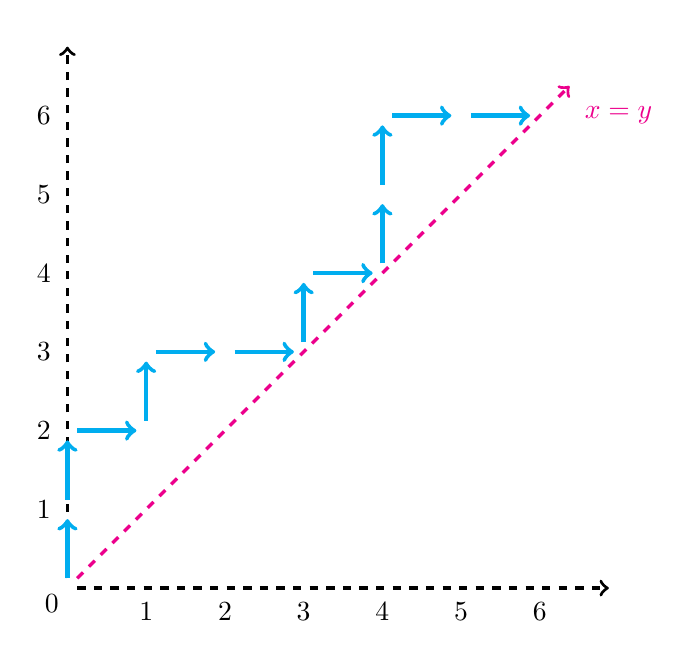
\begin{tikzpicture}[scale=1]
            \node (a) at (0, 0) {};
            \node (b) at (0, 7) {};
            \node (c) at (7, 0) {};
            \node (d) at (6.5, 6.5) {};
            \node (e) at (7, 6) [color = magenta]
                {$x = y$}; 
            \draw [dashed, very thick, ->] (a) to (b);
            \draw [dashed, very thick, ->] (a) to (c);
            \draw [dashed, very thick, ->]
                [color = magenta] (a) to (d);

            \node (1)  at (0,0)   {};
            \node (2)  at (0,1)   {};
            \node (3)  at (0,2)   {};
            \node (4)  at (1,2)   {};
            \node (5)  at (1,3)   {};
            \node (6)  at (2,3)   {};
            \node (7)  at (3,3)   {};
            \node (8)  at (3,4)   {};
            \node (9)  at (4,4)   {};
            \node (10) at (4,5)   {};
            \node (11) at (4,6)   {};
            \node (12) at (5,6)   {};
            \node (13) at (6,6)   {};
            \draw [->, ultra thick, color = cyan]
                (1)  to (2);
            \draw [->, ultra thick, color = cyan] 
                (2)  to (3);
            \draw [->, ultra thick, color = cyan]
                (3)  to (4);
            \draw [->, ultra thick, color = cyan]
                (4)  to (5);
            \draw [->, ultra thick, color = cyan]
                (5)  to (6);
            \draw [->, ultra thick, color = cyan]
                (6)  to (7);
            \draw [->, ultra thick, color = cyan]
                (7)  to (8);
            \draw [->, ultra thick, color = cyan]
                (8)  to (9);
            \draw [->, ultra thick, color = cyan]
                (9)  to (10);
            \draw [->, ultra thick, color = cyan]
                (10) to (11);
            \draw [->, ultra thick, color = cyan]
                (11) to (12);
            \draw [->, ultra thick, color = cyan]
                (12) to (13);

            \node at (-0.2, -0.2) {$0$};
            \node at (-0.3, 1)    {$1$};
            \node at (1, -0.3)    {$1$};
            \node at (-0.3, 2)    {$2$};
            \node at (2, -0.3)    {$2$};
            \node at (-0.3, 3)    {$3$};
            \node at (3, -0.3)    {$3$};
            \node at (-0.3, 4)    {$4$};
            \node at (4, -0.3)    {$4$};
            \node at (-0.3, 5)    {$5$};
            \node at (5, -0.3)    {$5$};
            \node at (-0.3, 6)    {$6$};
            \node at (6, -0.3)    {$6$};

        \end{tikzpicture}
    \end{center}
\end{example}

\begin{example}[$n = 6, \mathcal{D}_n \to \mathcal{PF'}_n$]
    ~\
    \begin{itemize}
        \item $w = 101011010010$
    \end{itemize}

    \begin{center}
        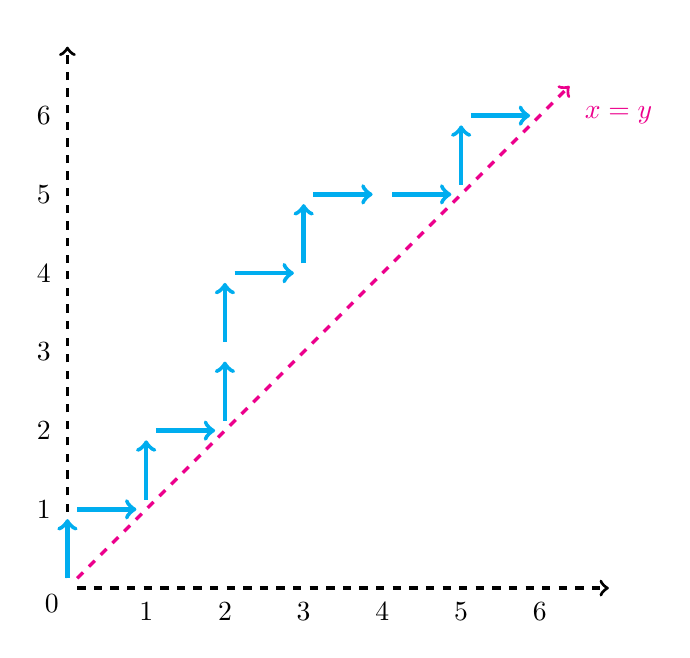
\begin{tikzpicture}[scale=1]
            \node (a) at (0, 0) {};
            \node (b) at (0, 7) {};
            \node (c) at (7, 0) {};
            \node (d) at (6.5, 6.5) {};
            \node (e) at (7, 6) [color = magenta]
                {$x = y$}; 
            \draw [dashed, very thick, ->] (a) to (b);
            \draw [dashed, very thick, ->] (a) to (c);
            \draw [dashed, very thick, ->]
                [color = magenta] (a) to (d);

            \node (1)  at (0,0)   {};
            \node (2)  at (0,1)   {};
            \node (3)  at (1,1)   {};
            \node (4)  at (1,2)   {};
            \node (5)  at (2,2)   {};
            \node (6)  at (2,3)   {};
            \node (7)  at (2,4)   {};
            \node (8)  at (3,4)   {};
            \node (9)  at (3,5)   {};
            \node (10) at (4,5)   {};
            \node (11) at (5,5)   {};
            \node (12) at (5,6)   {};
            \node (13) at (6,6)   {};
            \draw [->, ultra thick, color = cyan]
                (1)  to (2);
            \draw [->, ultra thick, color = cyan] 
                (2)  to (3);
            \draw [->, ultra thick, color = cyan]
                (3)  to (4);
            \draw [->, ultra thick, color = cyan]
                (4)  to (5);
            \draw [->, ultra thick, color = cyan]
                (5)  to (6);
            \draw [->, ultra thick, color = cyan]
                (6)  to (7);
            \draw [->, ultra thick, color = cyan]
                (7)  to (8);
            \draw [->, ultra thick, color = cyan]
                (8)  to (9);
            \draw [->, ultra thick, color = cyan]
                (9)  to (10);
            \draw [->, ultra thick, color = cyan]
                (10) to (11);
            \draw [->, ultra thick, color = cyan]
                (11) to (12);
            \draw [->, ultra thick, color = cyan]
                (12) to (13);

            \node at (-0.2, -0.2) {$0$};
            \node at (-0.3, 1)    {$1$};
            \node at (1, -0.3)    {$1$};
            \node at (-0.3, 2)    {$2$};
            \node at (2, -0.3)    {$2$};
            \node at (-0.3, 3)    {$3$};
            \node at (3, -0.3)    {$3$};
            \node at (-0.3, 4)    {$4$};
            \node at (4, -0.3)    {$4$};
            \node at (-0.3, 5)    {$5$};
            \node at (5, -0.3)    {$5$};
            \node at (-0.3, 6)    {$6$};
            \node at (6, -0.3)    {$6$};

        \end{tikzpicture}
    \end{center}
    \begin{itemize}
        \item Distances : 
            \subitem $s_1 = 0$
                \hspace{2cm} $a_1 = 1$
            \subitem $s_2 = 1$
                \hspace{2cm} $a_2 = 2$
            \subitem $s_3 = 2$
                \hspace{2cm} $a_3 = 3$
            \subitem $s_4 = 2$
                \hspace{2cm} $a_4 = 3$
            \subitem $s_5 = 3$
                \hspace{2cm} $a_5 = 4$
            \subitem $s_6 = 5$
                \hspace{2cm} $a_6 = 6$
        \item $f = (1, 2, 3, 3, 4, 6)$
    \end{itemize}
    
\end{example}

\subsection{Labeled Dyck Paths}

\begin{definition}[Labeled Dyck Path]
    A \emph{labeled Dyck word} is a word $w \in 
    \{0, \ldots, n\}^*$ such that :
    \begin{itemize}
        \item for each suffix $w'$ of $w$,
            $|w'|_{\neq 0} \geqslant |w'|_0$.
        \item $|w|_0 = |w|_{\neq 0}$.
        \item for each $i \in \{1, \ldots, n\}$, $w$ has 
            exactly one occurence of $i$.
        \item if $w_i \neq 0$ and $w_{i+1} \neq 0$,
            then $w_i < w_{i+1}$. That is, consecutive
            North steps have increasing labels.
    \end{itemize}
    A labeled Dyck word of length $2n$ can be represented
    as a path from $(0,0)$ to $(n,n)$, where each North
    step is associated to a label :
    \begin{itemize}
        \item Each $i \neq 0$ corresponds to a
            \emph{North step} $\uparrow$ labeled $i$.
        \item Each $0$ corresponds to an
            \emph{East step} $\rightarrow$.
    \end{itemize}
    Those paths are called \emph{labeled Dyck paths}.\\
    We denote by $\mathcal{LD}_n$ the set of labeled
    Dyck words of length $2n$.
\end{definition}

\begin{example}[$n = 5$]
    \begin{align*}
        &w_1 = 4051002030 \text{ is \emph{not} a labeled
            Dyck word, because }5 > 1.\\
        &w_2 = 4015002030 \text{ \emph{is} a labeled
            Dyck word :}\\
    \end{align*}
    \begin{center}
        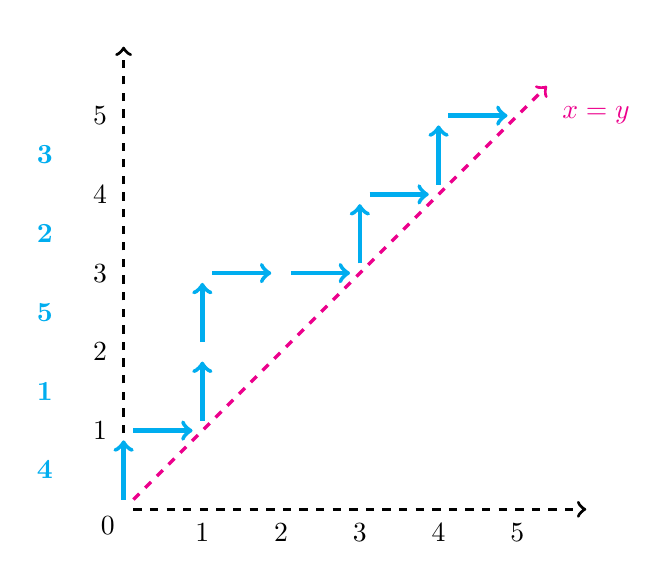
\begin{tikzpicture}[scale=1]
            \node (a) at (0, 0) {};
            \node (b) at (0, 6) {};
            \node (c) at (6, 0) {};
            \node (d) at (5.5, 5.5) {};
            \node (e) at (6, 5) [color = magenta]
                {$x = y$}; 
            \draw [dashed, very thick, ->] (a) to (b);
            \draw [dashed, very thick, ->] (a) to (c);
            \draw [dashed, very thick, ->]
                [color = magenta] (a) to (d);

            \node (1)  at (0,0)   {};
            \node (2)  at (0,1)   {};
            \node (3)  at (1,1)   {};
            \node (4)  at (1,2)   {};
            \node (5)  at (1,3)   {};
            \node (6)  at (2,3)   {};
            \node (7)  at (3,3)   {};
            \node (8)  at (3,4)   {};
            \node (9)  at (4,4)   {};
            \node (10) at (4,5)   {};
            \node (11) at (5,5)   {};
            \draw [->, ultra thick, color = cyan]
                (1)  to (2);
            \draw [->, ultra thick, color = cyan] 
                (2)  to (3);
            \draw [->, ultra thick, color = cyan]
                (3)  to (4);
            \draw [->, ultra thick, color = cyan]
                (4)  to (5);
            \draw [->, ultra thick, color = cyan]
                (5)  to (6);
            \draw [->, ultra thick, color = cyan]
                (6)  to (7);
            \draw [->, ultra thick, color = cyan]
                (7)  to (8);
            \draw [->, ultra thick, color = cyan]
                (8)  to (9);
            \draw [->, ultra thick, color = cyan]
                (9)  to (10);
            \draw [->, ultra thick, color = cyan]
                (10) to (11);

            \node at (-0.2, -0.2) {$0$};
            \node at (-0.3, 1)    {$1$};
            \node at (1, -0.3)    {$1$};
            \node at (-0.3, 2)    {$2$};
            \node at (2, -0.3)    {$2$};
            \node at (-0.3, 3)    {$3$};
            \node at (3, -0.3)    {$3$};
            \node at (-0.3, 4)    {$4$};
            \node at (4, -0.3)    {$4$};
            \node at (-0.3, 5)    {$5$};
            \node at (5, -0.3)    {$5$};

            \node [color = cyan] at (-1, 0.5) {\textbf{4}};
            \node [color = cyan] at (-1, 1.5) {\textbf{1}};
            \node [color = cyan] at (-1, 2.5) {\textbf{5}};
            \node [color = cyan] at (-1, 3.5) {\textbf{2}};
            \node [color = cyan] at (-1, 4.5) {\textbf{3}};

        \end{tikzpicture}
    \end{center}
\end{example}

\begin{theorem}
    Let $ld_n$ be the cardinal of $\mathcal{LD}_n$.
    We have $$ld_n = (n + 1)^{n - 1}$$.
\end{theorem}

\begin{example}[$n = 3$]
    $ld_n = 4^2 = 16$
    \begin{itemize}
        \item Word of shape $XXX000$ :
            \subitem $123000$
        \item Words of shape $XX0X00$ :
            \subitem $120300$
            \hspace{2cm} $130200$
            \hspace{2cm} $230100$
        \item Words of shape $XX00X0$ :
            \subitem $120030$
            \hspace{2cm} $130020$
            \hspace{2cm} $230010$
        \item Words of shape $X0XX00$ :
            \subitem $102300$
            \hspace{2cm} $201300$
            \hspace{2cm} $301200$
        \item Words of shape $X0X0X0$ :
            \subitem $102030$
            \hspace{2cm} $103020$
            \hspace{2cm} $201030$
            \subitem $203010$
            \hspace{2cm} $301020$
            \hspace{2cm} $302010$
    \end{itemize}
    
\end{example}

\begin{prop}
    This means we can create a \emph{bijection} between
    $\mathcal{PF}_n$ and $\mathcal{LD}_n$.
\end{prop}

\begin{proof}
    ~\
    \begin{itemize}
        \item $\mathcal{PF}_n \to \mathcal{LD}_n$ :
        Let $f = (a_1, \ldots, a_n) \in \mathcal{PF}_n$
        be our parking function. For $i \in \{1, \ldots,
        n\}$, we define $im_i$ : $\{j\ |\ a_j = i\}$. \\
        We then define $im_{i,1}, \ldots, im_{i,k_i}$ to be
        the elements of $im_i$ in increasing order.\\
        The corresponding labeled Dyck word will be \\
        $\underbrace{im_{1,1} \cdots im_{1,k_1}}_{im_1}0
         \underbrace{im_{2,1} \cdots im_{2,k_2}}_{im_2}0
         \cdots
         \underbrace{im_{n,1} \cdots im_{n,k_n}}_{im_n}0$.

        \item $\mathcal{LD}_n \to \mathcal{PF}_n$ :
        Let w be our labeled Dyck word, and consider its
        path representation. We define $s_i$ to be the
        distance between the segment from $(0, i-1)$ to
        $(0,i)$ and the $i^{th}$ North step.\\
        Then, let $label(i)$ be the label of the $i^{th}$
        North step, and $dist_i = \{label(j) | s_j = i\}$
        be the set of the labels of all North steps at
        distance $i$.\\
        Then, if $j \in dist_i$, let $a_j = i + 1$.\\
        The corresponding parking function is
        $(a_1, \ldots, a_n)$.
    \end{itemize}
\end{proof}

\begin{example}[$n = 6, \mathcal{PF}_n \to \mathcal{LD}_n$]
    ~\
    \begin{itemize}
        \item $f = (5, 2, 1, 4, 5, 1)$
            \subitem $im_1 = \{3, 6\}$
            \hspace{16mm} $im_2 = \{2\}$
            \hspace{24mm} $im_3 = \emptyset$
            \subitem $im_4 = \{4\}$
            \hspace{2cm} $im_5 = \{1, 5\}$
            \hspace{2cm} $im_6 = \emptyset$
        \item $w = 360200401500$
    \end{itemize}
    \begin{center}
        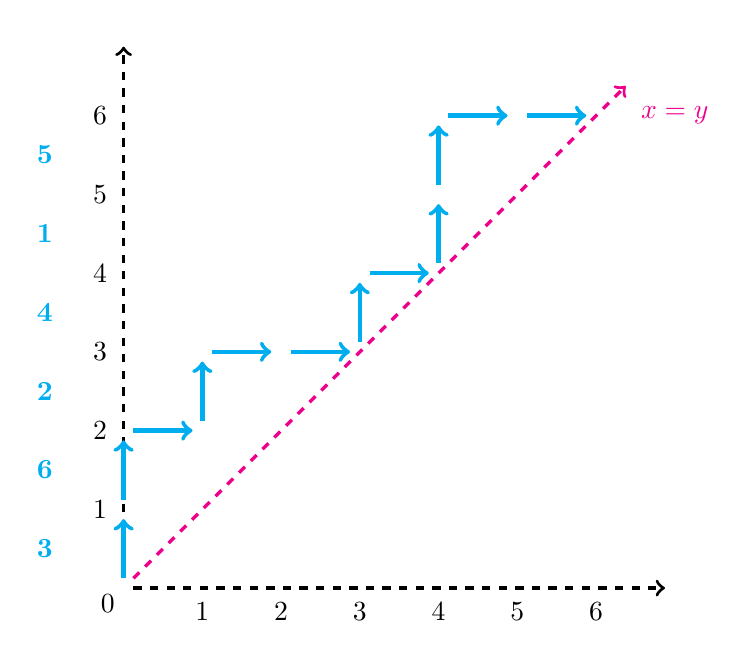
\begin{tikzpicture}[scale=1]
            \node (a) at (0, 0) {};
            \node (b) at (0, 7) {};
            \node (c) at (7, 0) {};
            \node (d) at (6.5, 6.5) {};
            \node (e) at (7, 6) [color = magenta]
                {$x = y$}; 
            \draw [dashed, very thick, ->] (a) to (b);
            \draw [dashed, very thick, ->] (a) to (c);
            \draw [dashed, very thick, ->]
                [color = magenta] (a) to (d);

            \node (1)  at (0,0)   {};
            \node (2)  at (0,1)   {};
            \node (3)  at (0,2)   {};
            \node (4)  at (1,2)   {};
            \node (5)  at (1,3)   {};
            \node (6)  at (2,3)   {};
            \node (7)  at (3,3)   {};
            \node (8)  at (3,4)   {};
            \node (9)  at (4,4)   {};
            \node (10) at (4,5)   {};
            \node (11) at (4,6)   {};
            \node (12) at (5,6)   {};
            \node (13) at (6,6)   {};
            \draw [->, ultra thick, color = cyan]
                (1)  to (2);
            \draw [->, ultra thick, color = cyan] 
                (2)  to (3);
            \draw [->, ultra thick, color = cyan]
                (3)  to (4);
            \draw [->, ultra thick, color = cyan]
                (4)  to (5);
            \draw [->, ultra thick, color = cyan]
                (5)  to (6);
            \draw [->, ultra thick, color = cyan]
                (6)  to (7);
            \draw [->, ultra thick, color = cyan]
                (7)  to (8);
            \draw [->, ultra thick, color = cyan]
                (8)  to (9);
            \draw [->, ultra thick, color = cyan]
                (9)  to (10);
            \draw [->, ultra thick, color = cyan]
                (10) to (11);
            \draw [->, ultra thick, color = cyan]
                (11) to (12);
            \draw [->, ultra thick, color = cyan]
                (12) to (13);

            \node at (-0.2, -0.2) {$0$};
            \node at (-0.3, 1)    {$1$};
            \node at (1, -0.3)    {$1$};
            \node at (-0.3, 2)    {$2$};
            \node at (2, -0.3)    {$2$};
            \node at (-0.3, 3)    {$3$};
            \node at (3, -0.3)    {$3$};
            \node at (-0.3, 4)    {$4$};
            \node at (4, -0.3)    {$4$};
            \node at (-0.3, 5)    {$5$};
            \node at (5, -0.3)    {$5$};
            \node at (-0.3, 6)    {$6$};
            \node at (6, -0.3)    {$6$};

            \node [color = cyan] at (-1, 0.5) {\textbf{3}};
            \node [color = cyan] at (-1, 1.5) {\textbf{6}};
            \node [color = cyan] at (-1, 2.5) {\textbf{2}};
            \node [color = cyan] at (-1, 3.5) {\textbf{4}};
            \node [color = cyan] at (-1, 4.5) {\textbf{1}};
            \node [color = cyan] at (-1, 5.5) {\textbf{5}};
        \end{tikzpicture}
    \end{center}
\end{example}

\begin{example}[$n = 6, \mathcal{LD}_n \to \mathcal{PF}_n$]
    ~\
    \begin{itemize}
        \item $w = 402560010030$
    \end{itemize}
    \begin{center}
        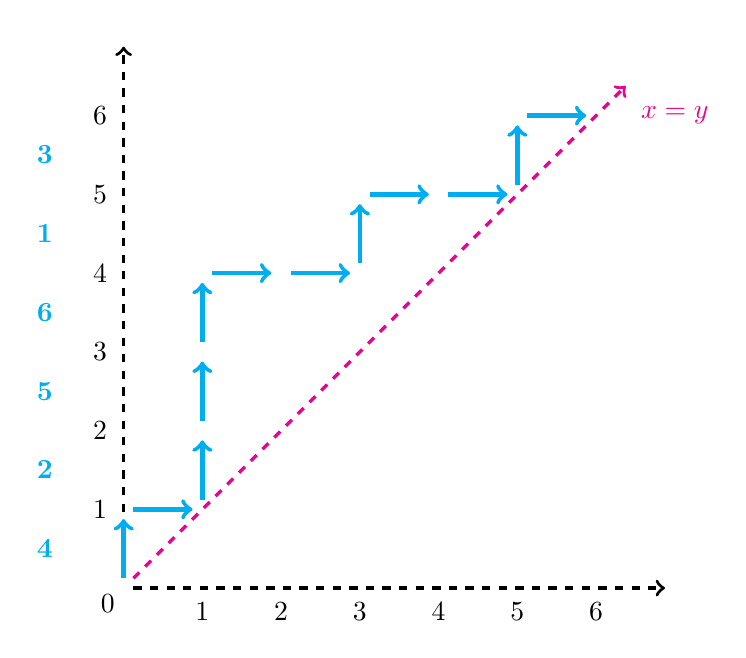
\begin{tikzpicture}[scale=1]
            \node (a) at (0, 0) {};
            \node (b) at (0, 7) {};
            \node (c) at (7, 0) {};
            \node (d) at (6.5, 6.5) {};
            \node (e) at (7, 6) [color = magenta]
                {$x = y$}; 
            \draw [dashed, very thick, ->] (a) to (b);
            \draw [dashed, very thick, ->] (a) to (c);
            \draw [dashed, very thick, ->]
                [color = magenta] (a) to (d);

            \node (1)  at (0,0)   {};
            \node (2)  at (0,1)   {};
            \node (3)  at (1,1)   {};
            \node (4)  at (1,2)   {};
            \node (5)  at (1,3)   {};
            \node (6)  at (1,4)   {};
            \node (7)  at (2,4)   {};
            \node (8)  at (3,4)   {};
            \node (9)  at (3,5)   {};
            \node (10) at (4,5)   {};
            \node (11) at (5,5)   {};
            \node (12) at (5,6)   {};
            \node (13) at (6,6)   {};
            \draw [->, ultra thick, color = cyan]
                (1)  to (2);
            \draw [->, ultra thick, color = cyan] 
                (2)  to (3);
            \draw [->, ultra thick, color = cyan]
                (3)  to (4);
            \draw [->, ultra thick, color = cyan]
                (4)  to (5);
            \draw [->, ultra thick, color = cyan]
                (5)  to (6);
            \draw [->, ultra thick, color = cyan]
                (6)  to (7);
            \draw [->, ultra thick, color = cyan]
                (7)  to (8);
            \draw [->, ultra thick, color = cyan]
                (8)  to (9);
            \draw [->, ultra thick, color = cyan]
                (9)  to (10);
            \draw [->, ultra thick, color = cyan]
                (10) to (11);
            \draw [->, ultra thick, color = cyan]
                (11) to (12);
            \draw [->, ultra thick, color = cyan]
                (12) to (13);

            \node at (-0.2, -0.2) {$0$};
            \node at (-0.3, 1)    {$1$};
            \node at (1, -0.3)    {$1$};
            \node at (-0.3, 2)    {$2$};
            \node at (2, -0.3)    {$2$};
            \node at (-0.3, 3)    {$3$};
            \node at (3, -0.3)    {$3$};
            \node at (-0.3, 4)    {$4$};
            \node at (4, -0.3)    {$4$};
            \node at (-0.3, 5)    {$5$};
            \node at (5, -0.3)    {$5$};
            \node at (-0.3, 6)    {$6$};
            \node at (6, -0.3)    {$6$};

            \node [color = cyan] at (-1, 0.5) {\textbf{4}};
            \node [color = cyan] at (-1, 1.5) {\textbf{2}};
            \node [color = cyan] at (-1, 2.5) {\textbf{5}};
            \node [color = cyan] at (-1, 3.5) {\textbf{6}};
            \node [color = cyan] at (-1, 4.5) {\textbf{1}};
            \node [color = cyan] at (-1, 5.5) {\textbf{3}};
        \end{tikzpicture}
    \end{center}

    \begin{itemize}
        \item Distances :
            \subitem $s_1 = 0$
            \hspace{2cm} $s_2 = 1$
            \hspace{2cm} $s_3 = 1$
            \subitem $s_4 = 1$
            \hspace{2cm} $s_5 = 3$
            \hspace{2cm} $s_6 = 5$
        \item Labels :
            \subitem $dist_0 = \{4\}$
            \hspace{2cm} $dist_1 = \{2, 5, 6\}$
            \hspace{2cm} $dist_2 = \emptyset$
            \subitem $dist_3 = \{1\}$
            \hspace{2cm} $dist_4 = \emptyset$
            \hspace{32mm} $dist_5 = \{3\}$
        \item $f = (4, 2, 6, 1, 2, 2)$
    \end{itemize}
\end{example}

\begin{rem}
    The primitive parking functions are exactly the
    parking functions corresponding to labeled Dyck paths
    where the $i^{th}$ North step is labeled $i$.
\end{rem}

\subsection{Dyck - Parking Posets}

\subsubsection{Primitive Dyck - Parking Posets}

\begin{definition}[$\gtrdot_d$]
    For $w$ and $w'$ two Dyck words, we say that $w$
    covers $w'$, written $w \gtrdot_d w'$, if
    $\exists w_1, w_2$ such that :
    \begin{itemize}
        \item $w = w_101w_2$
        \item $w' = w_110w_2$
    \end{itemize}  
\end{definition}

\begin{example}[$n = 7$]
    $10110011001100 \gtrdot_d 10110101001100$
    \begin{itemize}
        \item $w_1 = 10110$
        \item $w_2 = 1001100$
    \end{itemize}
    \begin{center}
        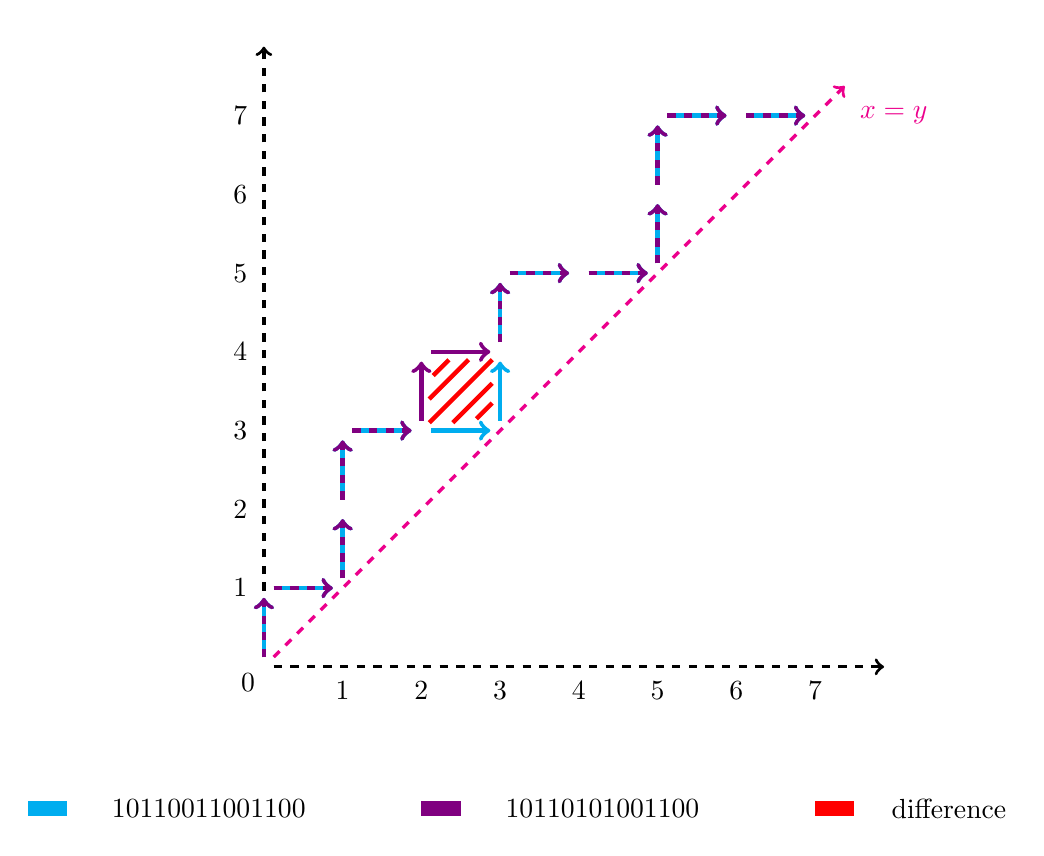
\begin{tikzpicture}[scale=1]
            \node (a) at (0, 0) {};
            \node (b) at (0, 8) {};
            \node (c) at (8, 0) {};
            \node (d) at (7.5, 7.5) {};
            \node (e) at (8, 7) [color = magenta]
                {$x = y$}; 
            \draw [dashed, very thick, ->] (a) to (b);
            \draw [dashed, very thick, ->] (a) to (c);
            \draw [dashed, very thick, ->]
                [color = magenta] (a) to (d);

            \node (1)  at (0,0)   {};
            \node (2)  at (0,1)   {};
            \node (3)  at (1,1)   {};
            \node (4)  at (1,2)   {};
            \node (5)  at (1,3)   {};
            \node (6)  at (2,3)   {};
            \node (7)  at (3,3)   {};
            \node (7b) at (2,4)   {};
            \node (8)  at (3,4)   {};
            \node (9)  at (3,5)   {};
            \node (10) at (4,5)   {};
            \node (11) at (5,5)   {};
            \node (12) at (5,6)   {};
            \node (13) at (5,7)   {};
            \node (14) at (6,7)   {};
            \node (15) at (7,7)   {};

            \draw [->, ultra thick, color = cyan]
                (1)  to (2);
            \draw [->, ultra thick, color = cyan] 
                (2)  to (3);
            \draw [->, ultra thick, color = cyan]
                (3)  to (4);
            \draw [->, ultra thick, color = cyan]
                (4)  to (5);
            \draw [->, ultra thick, color = cyan]
                (5)  to (6);
            \draw [->, ultra thick, color = cyan]
                (6)  to (7);
            \draw [->, ultra thick, color = cyan]
                (7)  to (8);
            \draw [->, ultra thick, color = cyan]
                (8)  to (9);
            \draw [->, ultra thick, color = cyan]
                (9)  to (10);
            \draw [->, ultra thick, color = cyan]
                (10) to (11);
            \draw [->, ultra thick, color = cyan]
                (11) to (12);
            \draw [->, ultra thick, color = cyan]
                (12) to (13);
            \draw [->, ultra thick, color = cyan]
                (13) to (14);
            \draw [->, ultra thick, color = cyan]
                (14) to (15);

            \draw [->, dashed, ultra thick, color = violet]
                (1)  to (2);
            \draw [->, dashed, ultra thick, color = violet] 
                (2)  to (3);
            \draw [->, dashed, ultra thick, color = violet]
                (3)  to (4);
            \draw [->, dashed, ultra thick, color = violet]
                (4)  to (5);
            \draw [->, dashed, ultra thick, color = violet]
                (5)  to (6);
            \draw [->, ultra thick, color = violet]
                (6)  to (7b);
            \draw [->, ultra thick, color = violet]
                (7b)  to (8);
            \draw [->, dashed, ultra thick, color = violet]
                (8)  to (9);
            \draw [->, dashed, ultra thick, color = violet]
                (9)  to (10);
            \draw [->, dashed, ultra thick, color = violet]
                (10) to (11);
            \draw [->, dashed, ultra thick, color = violet]
                (11) to (12);
            \draw [->, dashed, ultra thick, color = violet]
                (12) to (13);
            \draw [->, dashed, ultra thick, color = violet]
                (13) to (14);
            \draw [->, dashed, ultra thick, color = violet]
                (14) to (15);

            \node at (-0.2, -0.2) {$0$};
            \node at (-0.3, 1)    {$1$};
            \node at (1, -0.3)    {$1$};
            \node at (-0.3, 2)    {$2$};
            \node at (2, -0.3)    {$2$};
            \node at (-0.3, 3)    {$3$};
            \node at (3, -0.3)    {$3$};
            \node at (-0.3, 4)    {$4$};
            \node at (4, -0.3)    {$4$};
            \node at (-0.3, 5)    {$5$};
            \node at (5, -0.3)    {$5$};
            \node at (-0.3, 6)    {$6$};
            \node at (6, -0.3)    {$6$};
            \node at (-0.3, 7)    {$7$};
            \node at (7, -0.3)    {$7$};

            \draw[color = red, ultra thick]
                (2.1,3.1) -- (2.9,3.9);
            \draw[color = red, ultra thick]
                (2.1,3.4) -- (2.6,3.9);
            \draw[color = red, ultra thick]
                (2.15,3.7) -- (2.35,3.9);
            \draw[color = red, ultra thick]
                (2.4,3.1) -- (2.9,3.6);
            \draw[color = red, ultra thick]
                (2.7,3.15) -- (2.9,3.35);

            \fill[color = cyan] (-3,-1.9) rectangle
                (-2.5,-1.7);
            \node at (-0.7,-1.8) {$10110011001100$};
            \fill[color = violet] (2,-1.9) rectangle
            (2.5,-1.7);
            \node at (4.3,-1.8) {$10110101001100$};
            \fill[color = red] (7,-1.9) rectangle
            (7.5,-1.7);
            \node at (8.7,-1.8) {difference};
        \end{tikzpicture}
    \end{center}
\end{example}

\begin{rem}
    If $w_1 \gtrdot_d w_2$, then the path corresponding to
    $w_2$ is \emph{over} the path corresponding to $w_1$,
    and the \emph{difference} between the two paths is a
    square of size 1 by 1.
\end{rem}

\begin{prop}
    This covering relation defines a \emph{poset}
    for $\mathcal{D}_n$.
\end{prop}

\begin{example}[The poset of $\mathcal{D}_4$]
    ~\\
    \begin{center}
        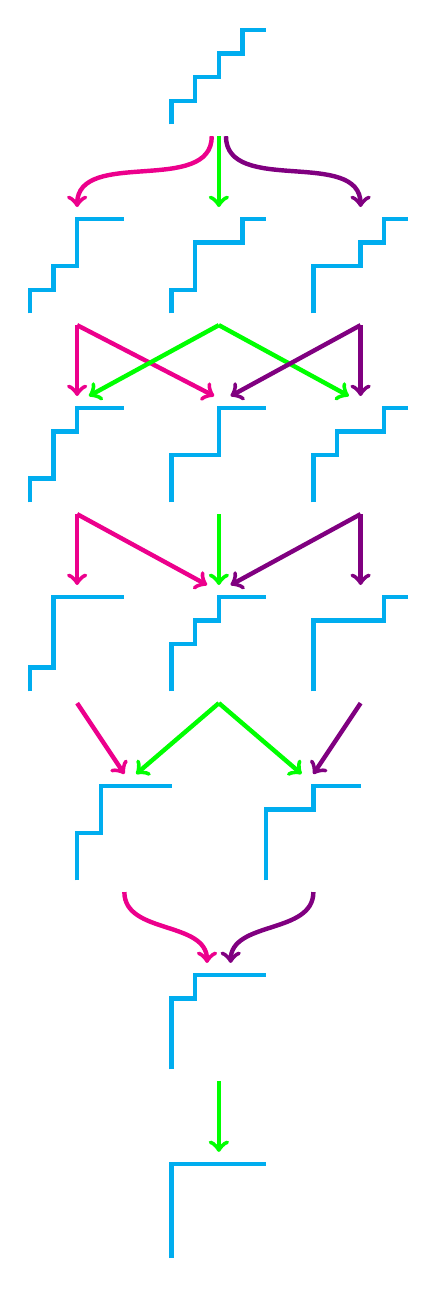
\begin{tikzpicture}[scale = 0.3]
            \draw [ultra thick, color = cyan] (0,0) -- (0,1)
                -- (0,2) -- (0,3) -- (0,4) -- (1,4) -- (2,4)
                -- (3,4) -- (4,4);

            \draw [ultra thick, color = cyan] (0,8) -- (0,9)
                -- (0,10) -- (0,11) -- (1,11) -- (1,12) -- (2,12)
                -- (3,12) -- (4,12);
                
            \draw [ultra thick, color = cyan] (-4,16) -- (-4,17)
                -- (-4,18) -- (-3,18) -- (-3,19) -- (-3,20)
                -- (-2,20) -- (-1,20) -- (0,20);

            \draw [ultra thick, color = cyan] (4,16) -- (4,17)
                -- (4,18) -- (4,19) -- (5,19) -- (6,19) -- (6,20)
                -- (7,20) -- (8,20);

            \draw [ultra thick, color = cyan] (-6,24) -- (-6,25)
                -- (-5,25) -- (-5,26) -- (-5,27) -- (-5,28)
                -- (-4,28) -- (-3,28) -- (-2,28);

            \draw [ultra thick, color = cyan] (0,24) -- (0,25)
                -- (0,26) -- (1,26) -- (1,27) -- (2,27) -- (2,28)
                -- (3,28) -- (4,28);

            \draw [ultra thick, color = cyan] (6,24) -- (6,25)
                -- (6,26) -- (6,27) -- (7,27) -- (8,27) -- (9,27)
                -- (9,28) -- (10,28);

            \draw [ultra thick, color = cyan] (-6,32) -- (-6,33)
                -- (-5,33) -- (-5,34) -- (-5,35) -- (-4,35)
                -- (-4,36) -- (-3,36) -- (-2,36);

            \draw [ultra thick, color = cyan] (0,32) -- (0,33)
                -- (0,34) -- (1,34) -- (2,34) -- (2,35) -- (2,36)
                -- (3,36) -- (4,36);

            \draw [ultra thick, color = cyan] (6,32) -- (6,33)
                -- (6,34) -- (7,34) -- (7,35) -- (8,35) -- (9,35)
                -- (9,36) -- (10,36);

            \draw [ultra thick, color = cyan] (-6,40) -- (-6,41)
                -- (-5,41) -- (-5,42) -- (-4,42) -- (-4,43)
                -- (-4,44) -- (-3,44) -- (-2,44);

            \draw [ultra thick, color = cyan] (0,40) -- (0,41)
                -- (1,41) -- (1,42) -- (1,43) -- (2,43) -- (3,43)
                -- (3,44) -- (4,44);

            \draw [ultra thick, color = cyan] (6,40) -- (6,41)
                -- (6,42) -- (7,42) -- (8,42) -- (8,43) -- (9,43)
                -- (9,44) -- (10,44);

            \draw [ultra thick, color = cyan] (0,48) -- (0,49)
                -- (1,49) -- (1,50) -- (2,50) -- (2,51) -- (3,51)
                -- (3,52) -- (4,52);


            \draw [->][out=-90,in=90, ultra thick] 
                [color=magenta](1.7,47.5) to (-4,44.5);
            \draw [->][color=magenta, ultra thick]
                (-4,39.5) to (-4,36.5);
            \draw [->][color=magenta, ultra thick]
                (-4,39.5) to (1.8,36.5); 
            \draw [->][color=magenta, ultra thick]
                (-4,31.5) to (-4,28.5);
            \draw [->][color=magenta, ultra thick]
                (-4,31.5) to (1.5,28.5);
            \draw [->][color=magenta, ultra thick]
                (-4,23.5) to (-2,20.5);
            \draw [->][out=-90,in=90, ultra thick] 
                [color=magenta](-2,15.5) to (1.5,12.5);
        

            \draw [->][out=-90,in=90, ultra thick]
                [color=green](2,47.5) to (2,44.5);
            \draw [->][color=green, ultra thick]
                (2,39.5) to (-3.5,36.5);
            \draw [->][color=green, ultra thick]
                (2,39.5) to (7.5,36.5);
            \draw [->][color=green, ultra thick]
                (2,31.5) to (2,28.5);
            \draw [->][color=green, ultra thick]
                (2,23.5) to (-1.5,20.5);
            \draw [->][color=green, ultra thick]
                (2,23.5) to (5.5,20.5);
            \draw [->][out=-90,in=90, ultra thick] 
                [color=green](2,7.5) to (2,4.5);
        
            \draw [->][out=-90,in=90, ultra thick]
                [color=violet](2.3,47.5) to (8,44.5);
            \draw [->][color=violet, ultra thick]
                (8,39.5) to (2.5,36.5);
            \draw [->][color=violet, ultra thick]
                (8,39.5) to (8,36.5);
            \draw [->][color=violet, ultra thick]
                (8,31.5) to (2.5,28.5);
            \draw [->][color=violet, ultra thick]
                (8,31.5) to (8,28.5);
            \draw [->][color=violet, ultra thick]
                (8,23.5) to (6,20.5);
            \draw [->][out=-90,in=90, ultra thick] 
                [color=violet](6,15.5) to (2.5,12.5);
        
        \end{tikzpicture}
        ~\\
        ~\\
        There are $\frac {1}{5} \binom{8}{4} = \frac{70}{5} = 14$
        elements in this poset.
    \end{center}
\end{example}

\begin{definition}[$\gtrdot'$]
    For $f$ and $g$ two primitive parking functions, we say
    that $f$ covers $g$, written $f \gtrdot' g$, if
    $\exists i$ such that :
    \begin{itemize}
        \item $f = (a_1, \ldots, a_{i-1}, a_i,\ \ \ \ 
            a_{i+1}, \ldots, a_n)$
        \item $g = (a_1, \ldots, a_{i-1}, a_i - 1, a_{i+1},
        \ldots, a_n)$
    \end{itemize}
\end{definition}

\begin{example}[$n = 6$]
    $(1, 1, 2, 3, 4, 5) \gtrdot' (1, 1, 2, 3, 3, 5)$    
\end{example}

\begin{prop}
    This covering relation defines a \emph{poset}
    for $\mathcal{PF'}_n$.
\end{prop}

\begin{example}[The poset of $\mathcal{PF'}_4$]
    ~\\
    \begin{center}
        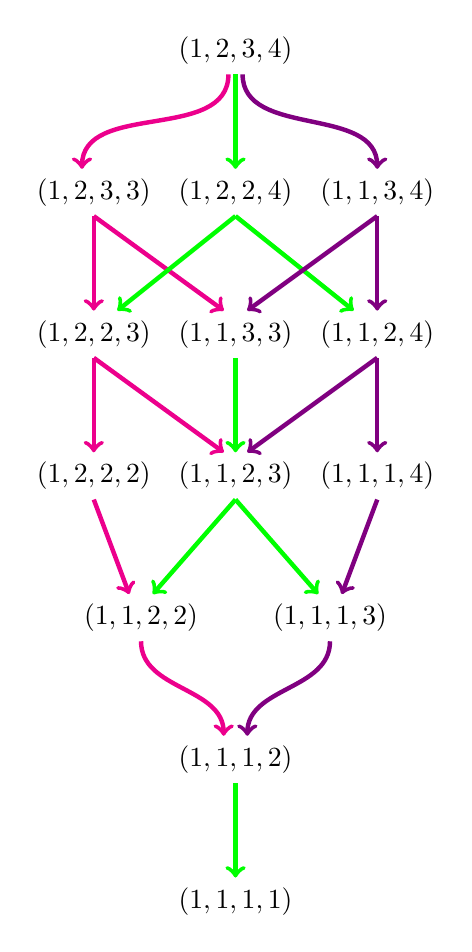
\begin{tikzpicture}[scale = 0.3]
            \node at (0,0)   {$(1,1,1,1)$};
            \node at (0,6)   {$(1,1,1,2)$};                
            \node at (-4,12) {$(1,1,2,2)$};
            \node at (4,12)  {$(1,1,1,3)$};
            \node at (-6,18) {$(1,2,2,2)$};
            \node at (0,18)  {$(1,1,2,3)$};
            \node at (6,18)  {$(1,1,1,4)$};
            \node at (-6,24) {$(1,2,2,3)$};
            \node at (0,24)  {$(1,1,3,3)$};
            \node at (6,24)  {$(1,1,2,4)$};
            \node at (-6,30) {$(1,2,3,3)$};
            \node at (0,30)  {$(1,2,2,4)$};
            \node at (6,30)  {$(1,1,3,4)$};
            \node at (0,36)  {$(1,2,3,4)$};


            \draw [->][out=-90,in=90, ultra thick] 
                [color=magenta](-0.3,35) to (-6.5,31);
            \draw [->][color=magenta, ultra thick]
                (-6,29) to (-6,25);
            \draw [->][color=magenta, ultra thick]
                (-6,29) to (-0.5,25); 
            \draw [->][color=magenta, ultra thick]
                (-6,23) to (-6,19);
            \draw [->][color=magenta, ultra thick]
                (-6,23) to (-0.5,19);
            \draw [->][color=magenta, ultra thick]
                (-6,17) to (-4.5,13);
            \draw [->][out=-90,in=90, ultra thick] 
                [color=magenta](-4,11) to (-0.5,7);
        

            \draw [->][out=-90,in=90, ultra thick]
                [color=green](0,35) to (0,31);
            \draw [->][color=green, ultra thick]
                (0,29) to (-5,25);
            \draw [->][color=green, ultra thick]
                (0,29) to (5,25);
            \draw [->][color=green, ultra thick]
                (0,23) to (0,19);
            \draw [->][color=green, ultra thick]
                (0,17) to (-3.5,13);
            \draw [->][color=green, ultra thick]
                (0,17) to (3.5,13);
            \draw [->][out=-90,in=90, ultra thick] 
                [color=green](0,5) to (0,1);
        
            \draw [->][out=-90,in=90, ultra thick]
                [color=violet](0.3,35) to (6,31);
            \draw [->][color=violet, ultra thick]
                (6,29) to (0.5,25);
            \draw [->][color=violet, ultra thick]
                (6,29) to (6,25);
            \draw [->][color=violet, ultra thick]
                (6,23) to (0.5,19);
            \draw [->][color=violet, ultra thick]
                (6,23) to (6,19);
            \draw [->][color=violet, ultra thick]
                (6,17) to (4.5,13);
            \draw [->][out=-90,in=90, ultra thick] 
                [color=violet](4,11) to (0.5,7);
        
        \end{tikzpicture}
        ~\\
        ~\\
        There are $\frac {1}{5} \binom{8}{4} = \frac{70}{5} = 14$
        elements in this poset.
    \end{center}
\end{example}

\begin{rem}
    The two posets are isomorphic, and one can be obtained by
    applying the aforementioned bijection to the other.
\end{rem}

\subsubsection{Classical Dyck - Parking Posets}

\begin{definition}[$\gtrdot_{ld}$]
    For $w$ and $w'$ two labeled Dyck words, we say
    that $w$ covers $w'$, written $w \gtrdot_{ld} w'$,
    if either :
    \begin{itemize}
        \item $\exists w_2, x, x', y$ such that :
            \subitem $x = x_1x_2 \cdots x_n$ has all 
            its digits $> 0$
            \subitem $x' = x$ where $y$ is correctly
            inserted regarding the order condition
            \subitem $y > 0$
            \subitem $w = x0yw_2$
            \subitem $w' = x'0w_2$
        \item $\exists w_1, w_2, x, x', y$ such that :
            \subitem $x = x_1x_2 \cdots x_n$ has all 
                its digits $> 0$
            \subitem $y > 0$
            \subitem $x' = x$ where $y$ is correctly
                inserted regarding the order condition
            \subitem $w = w_10x0yw_2$
            \subitem $w' = w_10x'0w_2$
        \item or $\exists w_1, w_2, y$ such that :
            \subitem $y > 0$
            \subitem $w = w_100yw_2$
            \subitem $w' = w_10y0w_2$
    \end{itemize}  
\end{definition}

\begin{example}[$n = 5$, first case]
    $1450302000 \gtrdot_{ld} 1345002000$
    \begin{itemize}
        \item $w_2 = 02000$
        \item $x = 145$
        \item $x' = 1345$
        \item $y = 3$
    \end{itemize}

    \begin{center}
        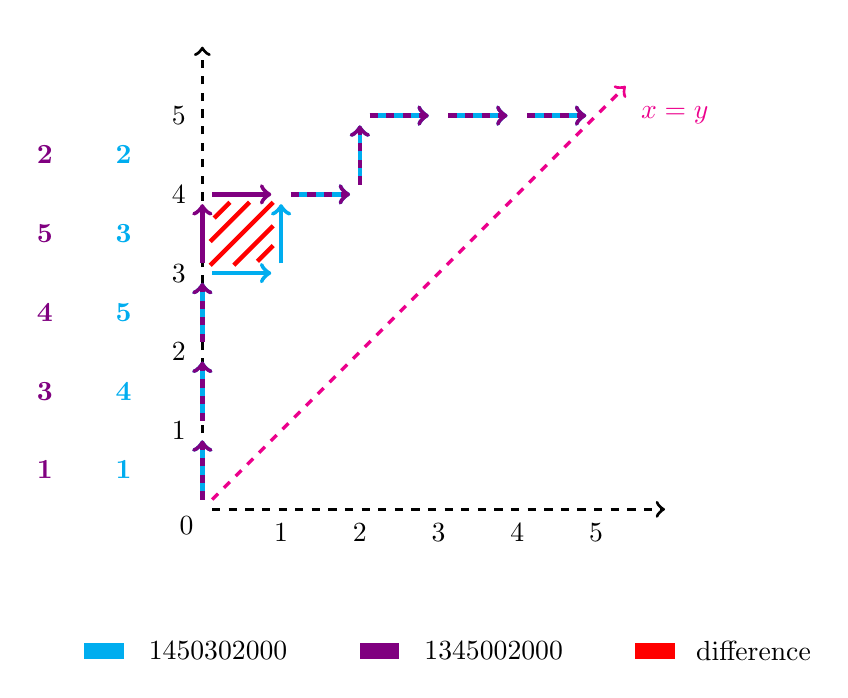
\begin{tikzpicture}[scale=1]
            \node (a) at (0, 0) {};
            \node (b) at (0, 6) {};
            \node (c) at (6, 0) {};
            \node (d) at (5.5, 5.5) {};
            \node (e) at (6, 5) [color = magenta]
                {$x = y$}; 
            \draw [dashed, very thick, ->] (a) to (b);
            \draw [dashed, very thick, ->] (a) to (c);
            \draw [dashed, very thick, ->]
                [color = magenta] (a) to (d);

            \node (1)  at (0,0)   {};
            \node (2)  at (0,1)   {};
            \node (3)  at (0,2)   {};
            \node (4)  at (0,3)   {};
            \node (5)  at (1,3)   {};
            \node (5b) at (0,4)   {};
            \node (6)  at (1,4)   {};
            \node (7)  at (2,4)   {};
            \node (8)  at (2,5)   {};
            \node (9)  at (3,5)   {};
            \node (10) at (4,5)   {};
            \node (11) at (5,5)   {};

            \draw [->, ultra thick, color = cyan]
                (1)  to (2);
            \draw [->, ultra thick, color = cyan] 
                (2)  to (3);
            \draw [->, ultra thick, color = cyan]
                (3)  to (4);
            \draw [->, ultra thick, color = cyan]
                (4)  to (5);
            \draw [->, ultra thick, color = cyan]
                (5)  to (6);
            \draw [->, ultra thick, color = cyan]
                (6)  to (7);
            \draw [->, ultra thick, color = cyan]
                (7)  to (8);
            \draw [->, ultra thick, color = cyan]
                (8)  to (9);
            \draw [->, ultra thick, color = cyan]
                (9)  to (10);
            \draw [->, ultra thick, color = cyan]
                (10) to (11);

            \draw [->, dashed, ultra thick, color = violet]
                (1)  to (2);
            \draw [->, dashed, ultra thick, color = violet] 
                (2)  to (3);
            \draw [->, dashed, ultra thick, color = violet]
                (3)  to (4);
            \draw [->, ultra thick, color = violet]
                (4)  to (5b);
            \draw [->, ultra thick, color = violet]
                (5b)  to (6);
            \draw [->, dashed, ultra thick, color = violet]
                (6)  to (7);
            \draw [->, dashed, ultra thick, color = violet]
                (7)  to (8);
            \draw [->, dashed, ultra thick, color = violet]
                (8)  to (9);
            \draw [->, dashed, ultra thick, color = violet]
                (9)  to (10);
            \draw [->, dashed, ultra thick, color = violet]
                (10) to (11);

            \node at (-0.2, -0.2) {$0$};
            \node at (-0.3, 1)    {$1$};
            \node at (1, -0.3)    {$1$};
            \node at (-0.3, 2)    {$2$};
            \node at (2, -0.3)    {$2$};
            \node at (-0.3, 3)    {$3$};
            \node at (3, -0.3)    {$3$};
            \node at (-0.3, 4)    {$4$};
            \node at (4, -0.3)    {$4$};
            \node at (-0.3, 5)    {$5$};
            \node at (5, -0.3)    {$5$};


            \node [color = cyan] at (-1, 0.5) {\textbf{1}};
            \node [color = cyan] at (-1, 1.5) {\textbf{4}};
            \node [color = cyan] at (-1, 2.5) {\textbf{5}};
            \node [color = cyan] at (-1, 3.5) {\textbf{3}};
            \node [color = cyan] at (-1, 4.5) {\textbf{2}};


            \node [color = violet] at (-2, 0.5) {\textbf{1}};
            \node [color = violet] at (-2, 1.5) {\textbf{3}};
            \node [color = violet] at (-2, 2.5) {\textbf{4}};
            \node [color = violet] at (-2, 3.5) {\textbf{5}};
            \node [color = violet] at (-2, 4.5) {\textbf{2}};

            \draw[color = red, ultra thick]
                (0.1,3.1) -- (0.9,3.9);
            \draw[color = red, ultra thick]
                (0.1,3.4) -- (0.6,3.9);
            \draw[color = red, ultra thick]
                (0.15,3.7) -- (0.35,3.9);
            \draw[color = red, ultra thick]
                (0.4,3.1) -- (0.9,3.6);
            \draw[color = red, ultra thick]
                (0.7,3.15) -- (0.9,3.35);

            \fill[color = cyan] (-1,-1.9) rectangle
                (-1.5,-1.7);
            \node at (0.2,-1.8) {$1450302000$};
            \fill[color = violet] (2,-1.9) rectangle
                (2.5,-1.7);
            \node at (3.7,-1.8) {$1345002000$};
            \fill[color = red] (6,-1.9) rectangle
                (5.5,-1.7);
            \node at (7,-1.8) {difference};
        \end{tikzpicture}
    \end{center}
\end{example}

\begin{example}[$n = 5$, second case]
    $4015030200 \gtrdot_{ld} 4013500200$
    \begin{itemize}
        \item $w_1 = 4$
        \item $w_2 = 0200$
        \item $x = 15$
        \item $x' = 135$
        \item $y = 3$
    \end{itemize}

    \begin{center}
        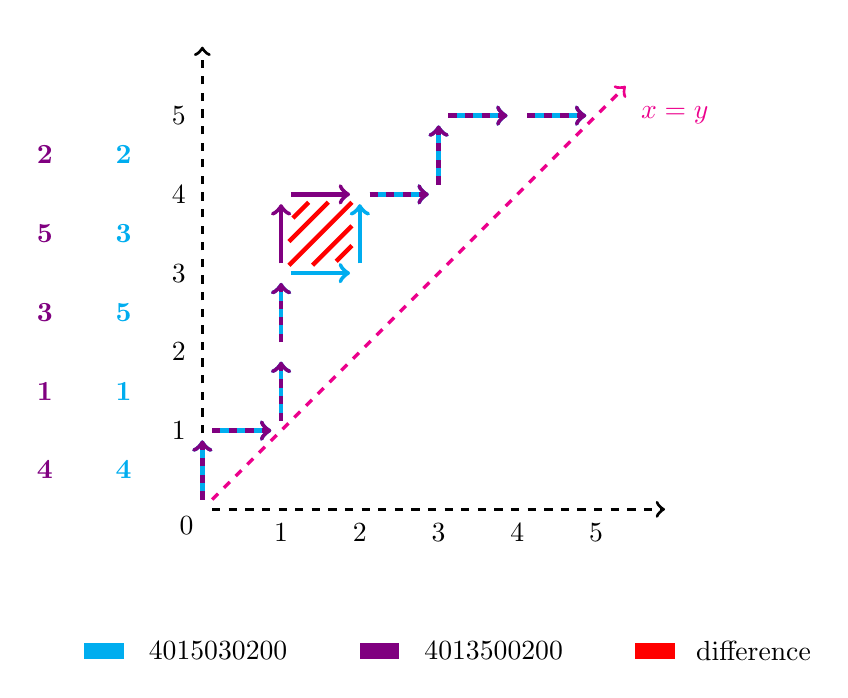
\begin{tikzpicture}[scale=1]
            \node (a) at (0, 0) {};
            \node (b) at (0, 6) {};
            \node (c) at (6, 0) {};
            \node (d) at (5.5, 5.5) {};
            \node (e) at (6, 5) [color = magenta]
                {$x = y$}; 
            \draw [dashed, very thick, ->] (a) to (b);
            \draw [dashed, very thick, ->] (a) to (c);
            \draw [dashed, very thick, ->]
                [color = magenta] (a) to (d);

            \node (1)  at (0,0)   {};
            \node (2)  at (0,1)   {};
            \node (3)  at (1,1)   {};
            \node (4)  at (1,2)   {};
            \node (5)  at (1,3)   {};
            \node (6)  at (2,3)   {};
            \node (6b) at (1,4)   {};
            \node (7)  at (2,4)   {};
            \node (8)  at (3,4)   {};
            \node (9)  at (3,5)   {};
            \node (10) at (4,5)   {};
            \node (11) at (5,5)   {};

            \draw [->, ultra thick, color = cyan]
                (1)  to (2);
            \draw [->, ultra thick, color = cyan] 
                (2)  to (3);
            \draw [->, ultra thick, color = cyan]
                (3)  to (4);
            \draw [->, ultra thick, color = cyan]
                (4)  to (5);
            \draw [->, ultra thick, color = cyan]
                (5)  to (6);
            \draw [->, ultra thick, color = cyan]
                (6)  to (7);
            \draw [->, ultra thick, color = cyan]
                (7)  to (8);
            \draw [->, ultra thick, color = cyan]
                (8)  to (9);
            \draw [->, ultra thick, color = cyan]
                (9)  to (10);
            \draw [->, ultra thick, color = cyan]
                (10) to (11);

            \draw [->, dashed, ultra thick, color = violet]
                (1)  to (2);
            \draw [->, dashed, ultra thick, color = violet] 
                (2)  to (3);
            \draw [->, dashed, ultra thick, color = violet]
                (3)  to (4);
            \draw [->, dashed, ultra thick, color = violet]
                (4)  to (5);
            \draw [->, ultra thick, color = violet]
                (5)  to (6b);
            \draw [->, ultra thick, color = violet]
                (6b)  to (7);
            \draw [->, dashed, ultra thick, color = violet]
                (7)  to (8);
            \draw [->, dashed, ultra thick, color = violet]
                (8)  to (9);
            \draw [->, dashed, ultra thick, color = violet]
                (9)  to (10);
            \draw [->, dashed, ultra thick, color = violet]
                (10) to (11);

            \node at (-0.2, -0.2) {$0$};
            \node at (-0.3, 1)    {$1$};
            \node at (1, -0.3)    {$1$};
            \node at (-0.3, 2)    {$2$};
            \node at (2, -0.3)    {$2$};
            \node at (-0.3, 3)    {$3$};
            \node at (3, -0.3)    {$3$};
            \node at (-0.3, 4)    {$4$};
            \node at (4, -0.3)    {$4$};
            \node at (-0.3, 5)    {$5$};
            \node at (5, -0.3)    {$5$};


            \node [color = cyan] at (-1, 0.5) {\textbf{4}};
            \node [color = cyan] at (-1, 1.5) {\textbf{1}};
            \node [color = cyan] at (-1, 2.5) {\textbf{5}};
            \node [color = cyan] at (-1, 3.5) {\textbf{3}};
            \node [color = cyan] at (-1, 4.5) {\textbf{2}};

            \node [color = violet] at (-2, 0.5) {\textbf{4}};
            \node [color = violet] at (-2, 1.5) {\textbf{1}};
            \node [color = violet] at (-2, 2.5) {\textbf{3}};
            \node [color = violet] at (-2, 3.5) {\textbf{5}};
            \node [color = violet] at (-2, 4.5) {\textbf{2}};

            \draw[color = red, ultra thick]
                (1.1,3.1) -- (1.9,3.9);
            \draw[color = red, ultra thick]
                (1.1,3.4) -- (1.6,3.9);
            \draw[color = red, ultra thick]
                (1.15,3.7) -- (1.35,3.9);
            \draw[color = red, ultra thick]
                (1.4,3.1) -- (1.9,3.6);
            \draw[color = red, ultra thick]
                (1.7,3.15) -- (1.9,3.35);

            \fill[color = cyan] (-1,-1.9) rectangle
                (-1.5,-1.7);
            \node at (0.2,-1.8) {$4015030200$};
            \fill[color = violet] (2,-1.9) rectangle
                (2.5,-1.7);
            \node at (3.7,-1.8) {$4013500200$};
            \fill[color = red] (6,-1.9) rectangle
                (5.5,-1.7);
            \node at (7,-1.8) {difference};
        \end{tikzpicture}
    \end{center}
\end{example}

\begin{example}[$n = 5$, third case]
    $4015003020 \gtrdot_{ld} 4015030020$
    \begin{itemize}
        \item $w_1 = 4015$
        \item $w_2 = 020$
        \item $y = 3$
    \end{itemize}

    \begin{center}
        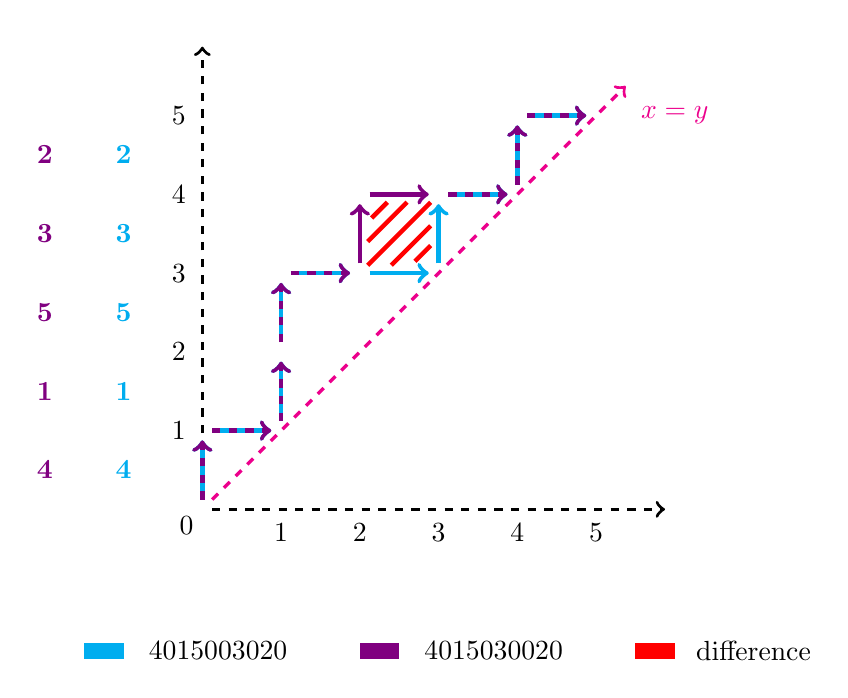
\begin{tikzpicture}[scale=1]
            \node (a) at (0, 0) {};
            \node (b) at (0, 6) {};
            \node (c) at (6, 0) {};
            \node (d) at (5.5, 5.5) {};
            \node (e) at (6, 5) [color = magenta]
                {$x = y$}; 
            \draw [dashed, very thick, ->] (a) to (b);
            \draw [dashed, very thick, ->] (a) to (c);
            \draw [dashed, very thick, ->]
                [color = magenta] (a) to (d);

            \node (1)  at (0,0)   {};
            \node (2)  at (0,1)   {};
            \node (3)  at (1,1)   {};
            \node (4)  at (1,2)   {};
            \node (5)  at (1,3)   {};
            \node (6)  at (2,3)   {};
            \node (7)  at (3,3)   {};
            \node (7b) at (2,4)   {};
            \node (8)  at (3,4)   {};
            \node (9)  at (4,4)   {};
            \node (10) at (4,5)   {};
            \node (11) at (5,5)   {};

            \draw [->, ultra thick, color = cyan]
                (1)  to (2);
            \draw [->, ultra thick, color = cyan] 
                (2)  to (3);
            \draw [->, ultra thick, color = cyan]
                (3)  to (4);
            \draw [->, ultra thick, color = cyan]
                (4)  to (5);
            \draw [->, ultra thick, color = cyan]
                (5)  to (6);
            \draw [->, ultra thick, color = cyan]
                (6)  to (7);
            \draw [->, ultra thick, color = cyan]
                (7)  to (8);
            \draw [->, ultra thick, color = cyan]
                (8)  to (9);
            \draw [->, ultra thick, color = cyan]
                (9)  to (10);
            \draw [->, ultra thick, color = cyan]
                (10) to (11);

            \draw [->, dashed, ultra thick, color = violet]
                (1)  to (2);
            \draw [->, dashed, ultra thick, color = violet] 
                (2)  to (3);
            \draw [->, dashed, ultra thick, color = violet]
                (3)  to (4);
            \draw [->, dashed, ultra thick, color = violet]
                (4)  to (5);
            \draw [->, dashed, ultra thick, color = violet]
                (5)  to (6);
            \draw [->, ultra thick, color = violet]
                (6)  to (7b);
            \draw [->, ultra thick, color = violet]
                (7b)  to (8);
            \draw [->, dashed, ultra thick, color = violet]
                (8)  to (9);
            \draw [->, dashed, ultra thick, color = violet]
                (9)  to (10);
            \draw [->, dashed, ultra thick, color = violet]
                (10) to (11);

            \node at (-0.2, -0.2) {$0$};
            \node at (-0.3, 1)    {$1$};
            \node at (1, -0.3)    {$1$};
            \node at (-0.3, 2)    {$2$};
            \node at (2, -0.3)    {$2$};
            \node at (-0.3, 3)    {$3$};
            \node at (3, -0.3)    {$3$};
            \node at (-0.3, 4)    {$4$};
            \node at (4, -0.3)    {$4$};
            \node at (-0.3, 5)    {$5$};
            \node at (5, -0.3)    {$5$};


            \node [color = cyan] at (-1, 0.5) {\textbf{4}};
            \node [color = cyan] at (-1, 1.5) {\textbf{1}};
            \node [color = cyan] at (-1, 2.5) {\textbf{5}};
            \node [color = cyan] at (-1, 3.5) {\textbf{3}};
            \node [color = cyan] at (-1, 4.5) {\textbf{2}};

            \node [color = violet] at (-2, 0.5) {\textbf{4}};
            \node [color = violet] at (-2, 1.5) {\textbf{1}};
            \node [color = violet] at (-2, 2.5) {\textbf{5}};
            \node [color = violet] at (-2, 3.5) {\textbf{3}};
            \node [color = violet] at (-2, 4.5) {\textbf{2}};

            \draw[color = red, ultra thick]
                (2.1,3.1) -- (2.9,3.9);
            \draw[color = red, ultra thick]
                (2.1,3.4) -- (2.6,3.9);
            \draw[color = red, ultra thick]
                (2.15,3.7) -- (2.35,3.9);
            \draw[color = red, ultra thick]
                (2.4,3.1) -- (2.9,3.6);
            \draw[color = red, ultra thick]
                (2.7,3.15) -- (2.9,3.35);

            \fill[color = cyan] (-1,-1.9) rectangle
                (-1.5,-1.7);
            \node at (0.2,-1.8) {$4015003020$};
            \fill[color = violet] (2,-1.9) rectangle
                (2.5,-1.7);
            \node at (3.7,-1.8) {$4015030020$};
            \fill[color = red] (6,-1.9) rectangle
                (5.5,-1.7);
            \node at (7,-1.8) {difference};
        \end{tikzpicture}
    \end{center}
\end{example}

\begin{rem}
    If $w_1 \gtrdot_{ld} w_2$, then the path corresponding to
    $w_2$ is \emph{over} the path corresponding to $w_1$,
    and the \emph{difference} between the two paths is a
    square of size 1 by 1.\\
    Furthermore, the labeling can be seen as follows :
    if one has to merge two sequences of North steps of $w_1$
    to make $w_2$, then the merging will be made by ordering the
    corresponding labels.
\end{rem}

\begin{prop}
    This covering relation defines a \emph{poset}
    for $\mathcal{LD}_n$.
\end{prop}

\begin{example}[The poset of $\mathcal{LD}_3$]
    ~\\
    \begin{center}
        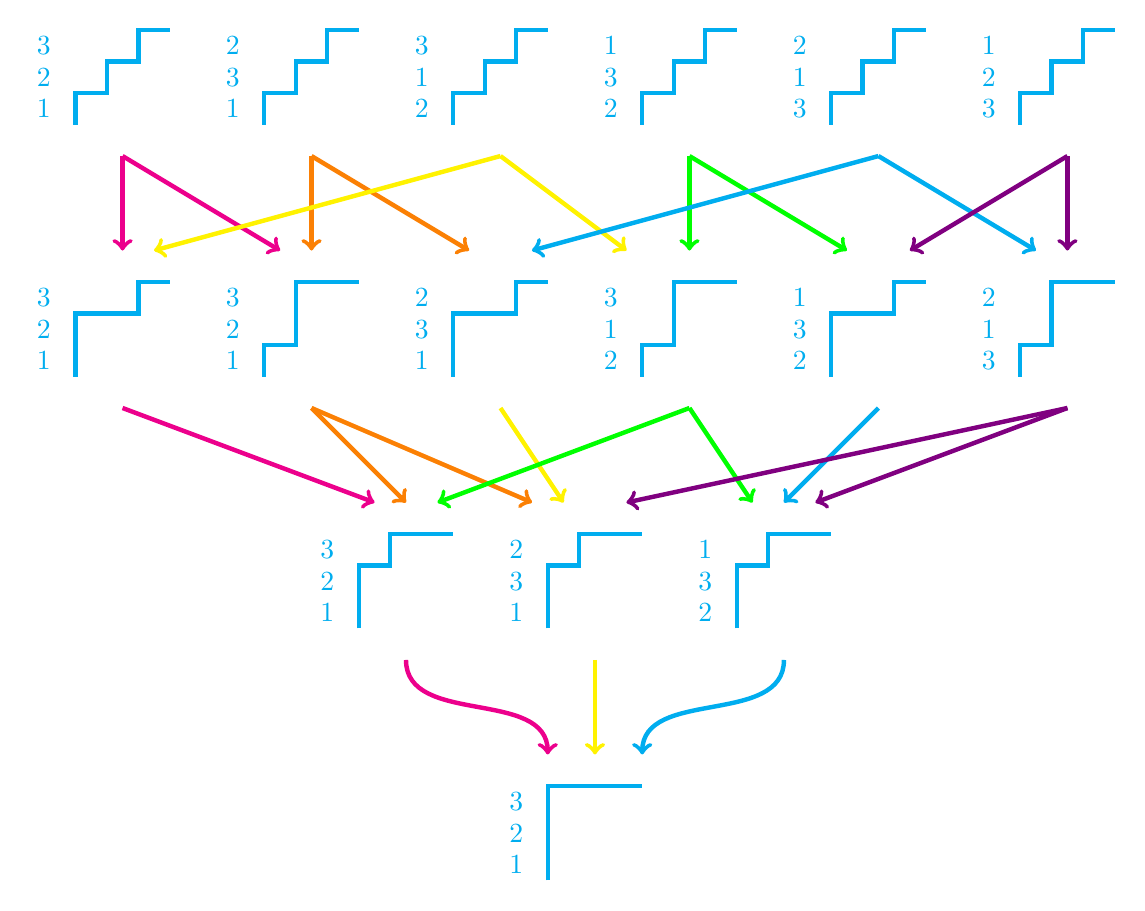
\begin{tikzpicture}[scale = 0.4]
            \draw [ultra thick, color = cyan] (0,0) -- (0,1)
                -- (0,2) -- (0,3) -- (1,3) -- (2,3) -- (3,3);
            \node[color = cyan] at (-1,0.5) {$1$};
            \node[color = cyan] at (-1,1.5) {$2$};
            \node[color = cyan] at (-1,2.5) {$3$};

            \draw [ultra thick, color = cyan] (-6,8) -- (-6,9)
                -- (-6,10) -- (-5,10) -- (-5,11) -- (-4,11)
                -- (-3,11);
            \node[color = cyan] at (-7,8.5) {$1$};
            \node[color = cyan] at (-7,9.5) {$2$};
            \node[color = cyan] at (-7,10.5) {$3$};
                
            \draw [ultra thick, color = cyan] (0,8) -- (0,9)
                -- (0,10) -- (1,10) -- (1,11) -- (2,11)
                -- (3,11);
            \node[color = cyan] at (-1,8.5) {$1$};
            \node[color = cyan] at (-1,9.5) {$3$};
            \node[color = cyan] at (-1,10.5) {$2$};

            \draw [ultra thick, color = cyan] (6,8) -- (6,9)
                -- (6,10) -- (7,10) -- (7,11) -- (8,11)
                 -- (9,11);
            \node[color = cyan] at (5,8.5) {$2$};
            \node[color = cyan] at (5,9.5) {$3$};
            \node[color = cyan] at (5,10.5) {$1$};

            \draw [ultra thick, color = cyan] (-15,16) -- (-15,17)
                -- (-15,18) -- (-14,18) -- (-13,18) -- (-13,19)
                -- (-12,19);
            \node[color = cyan] at (-16,16.5) {$1$};
            \node[color = cyan] at (-16,17.5) {$2$};
            \node[color = cyan] at (-16,18.5) {$3$};

            \draw [ultra thick, color = cyan] (-9,16) -- (-9,17)
                -- (-8,17) -- (-8,18) -- (-8,19) -- (-7,19)
                -- (-6,19);
            \node[color = cyan] at (-10,16.5) {$1$};
            \node[color = cyan] at (-10,17.5) {$2$};
            \node[color = cyan] at (-10,18.5) {$3$};

            \draw [ultra thick, color = cyan] (-3,16) -- (-3,17)
                -- (-3,18) -- (-2,18) -- (-1,18) -- (-1,19)
                -- (0,19);
            \node[color = cyan] at (-4,16.5) {$1$};
            \node[color = cyan] at (-4,17.5) {$3$};
            \node[color = cyan] at (-4,18.5) {$2$};

            \draw [ultra thick, color = cyan] (3,16) -- (3,17)
                -- (4,17) -- (4,18) -- (4,19) -- (5,19)
                -- (6,19);
            \node[color = cyan] at (2,16.5) {$2$};
            \node[color = cyan] at (2,17.5) {$1$};
            \node[color = cyan] at (2,18.5) {$3$};

            \draw [ultra thick, color = cyan] (9,16) -- (9,17)
                -- (9,18) -- (10,18) -- (11,18) -- (11,19)
                -- (12,19);
            \node[color = cyan] at (8,16.5) {$2$};
            \node[color = cyan] at (8,17.5) {$3$};
            \node[color = cyan] at (8,18.5) {$1$};

            \draw [ultra thick, color = cyan] (15,16) -- (15,17)
                -- (16,17) -- (16,18) -- (16,19) -- (17,19)
                -- (18,19);
            \node[color = cyan] at (14,16.5) {$3$};
            \node[color = cyan] at (14,17.5) {$1$};
            \node[color = cyan] at (14,18.5) {$2$};

            \draw [ultra thick, color = cyan] (-15,24) -- (-15,25)
                -- (-14,25) -- (-14,26) -- (-13,26) -- (-13,27)
                -- (-12,27);
            \node[color = cyan] at (-16,24.5) {$1$};
            \node[color = cyan] at (-16,25.5) {$2$};
            \node[color = cyan] at (-16,26.5) {$3$};

            \draw [ultra thick, color = cyan] (-9,24) -- (-9,25)
                -- (-8,25) -- (-8,26) -- (-7,26) -- (-7,27)
                -- (-6,27);
            \node[color = cyan] at (-10,24.5) {$1$};
            \node[color = cyan] at (-10,25.5) {$3$};
            \node[color = cyan] at (-10,26.5) {$2$};

            \draw [ultra thick, color = cyan] (-3,24) -- (-3,25)
                -- (-2,25) -- (-2,26) -- (-1,26) -- (-1,27)
                -- (0,27);
            \node[color = cyan] at (-4,24.5) {$2$};
            \node[color = cyan] at (-4,25.5) {$1$};
            \node[color = cyan] at (-4,26.5) {$3$};


            \draw [ultra thick, color = cyan] (3,24) -- (3,25)
                -- (4,25) -- (4,26) -- (5,26) -- (5,27)
                -- (6,27);
            \node[color = cyan] at (2,24.5) {$2$};
            \node[color = cyan] at (2,25.5) {$3$};
            \node[color = cyan] at (2,26.5) {$1$};

            \draw [ultra thick, color = cyan] (9,24) -- (9,25)
                -- (10,25) -- (10,26) -- (11,26) -- (11,27)
                -- (12,27);
            \node[color = cyan] at (8,24.5) {$3$};
            \node[color = cyan] at (8,25.5) {$1$};
            \node[color = cyan] at (8,26.5) {$2$};

            \draw [ultra thick, color = cyan] (15,24) -- (15,25)
                -- (16,25) -- (16,26) -- (17,26) -- (17,27)
                -- (18,27);
            \node[color = cyan] at (14,24.5) {$3$};
            \node[color = cyan] at (14,25.5) {$2$};
            \node[color = cyan] at (14,26.5) {$1$};

            \draw [->][color=magenta, ultra thick]
                (-13.5,23) to (-13.5,20);
            \draw [->][color=magenta, ultra thick]
                (-13.5,23) to (-8.5,20);
            \draw [->][color=magenta, ultra thick]
                (-13.5,15) to (-5.5,12); 
            \draw [->][out=-90,in=90, ultra thick] 
                [color=magenta](-4.5,7) to (0,4);

            \draw [->][color=brown!7!orange, ultra thick]
                (-7.5,23) to (-7.5,20);
            \draw [->][color=brown!7!orange, ultra thick]
                (-7.5,23) to (-2.5,20);
            \draw [->][color=brown!7!orange, ultra thick]
                (-7.5,15) to (-4.5,12);
            \draw [->][color=brown!7!orange, ultra thick]
                (-7.5,15) to (-0.5,12);

            \draw [->][color=yellow, ultra thick]
                (-1.5,23) to (-12.5,20);
            \draw [->][color=yellow, ultra thick]
                (-1.5,23) to (2.5,20);
            \draw [->][color=yellow, ultra thick]
                (-1.5,15) to (0.5,12); 
            \draw [->][out=-90,in=90, ultra thick] 
                [color=yellow](1.5,7) to (1.5,4);

            \draw [->][color = green,  ultra thick]
                (4.5,23) to (4.5,20);
            \draw [->][color=green, ultra thick]
                (4.5,23) to (9.5,20);
            \draw [->][color=green, ultra thick]
                (4.5,15) to (-3.5,12);
            \draw [->][color=green, ultra thick]
                (4.5,15) to (6.5,12);
        
            \draw [->][color=cyan, ultra thick]
                (10.5,23) to (-0.5,20);
            \draw [->][color=cyan, ultra thick]
                (10.5,23) to (15.5,20);
            \draw [->][color=cyan, ultra thick]
                (10.5,15) to (7.5,12); 
            \draw [->][out=-90,in=90, ultra thick] 
                [color=cyan](7.5,7) to (3,4);

            \draw [->][color=violet, ultra thick]
                (16.5,23) to (11.5,20);
            \draw [->][color=violet, ultra thick]
                (16.5,23) to (16.5,20);
            \draw [->][color=violet, ultra thick]
                (16.5,15) to (2.5,12);
            \draw [->][color=violet, ultra thick]
                (16.5,15) to (8.5,12);
        
        \end{tikzpicture}
        ~\\
        ~\\
        There are $4^2 = 16$ elements in this poset.
    \end{center}
\end{example}

\begin{definition}[$\gtrdot$]
    For $f$ and $g$ two parking functions, we say
    that $f$ covers $g$, written $f \gtrdot g$, if
    $\exists i$ such that :
    \begin{itemize}
        \item $f = (a_1, \ldots, a_{i-1}, a_i,\ \ \ \ 
            a_{i+1}, \ldots, a_n)$
        \item $g = (a_1, \ldots, a_{i-1}, a_i - 1, a_{i+1},
        \ldots, a_n)$
    \end{itemize}
    That is, the same relation as for primitive
    parking functions.
\end{definition}

\begin{example}[$n = 6$]
    $(2, 1, 5, 3, 1, 4) \gtrdot (2, 1, 5, 2, 1, 4)$    
\end{example}

\begin{prop}
    This covering relation defines a \emph{poset}
    for $\mathcal{PF}_n$.
\end{prop}

\begin{example}[The poset of $\mathcal{PF}_3$]
    ~\\
    \begin{center}
        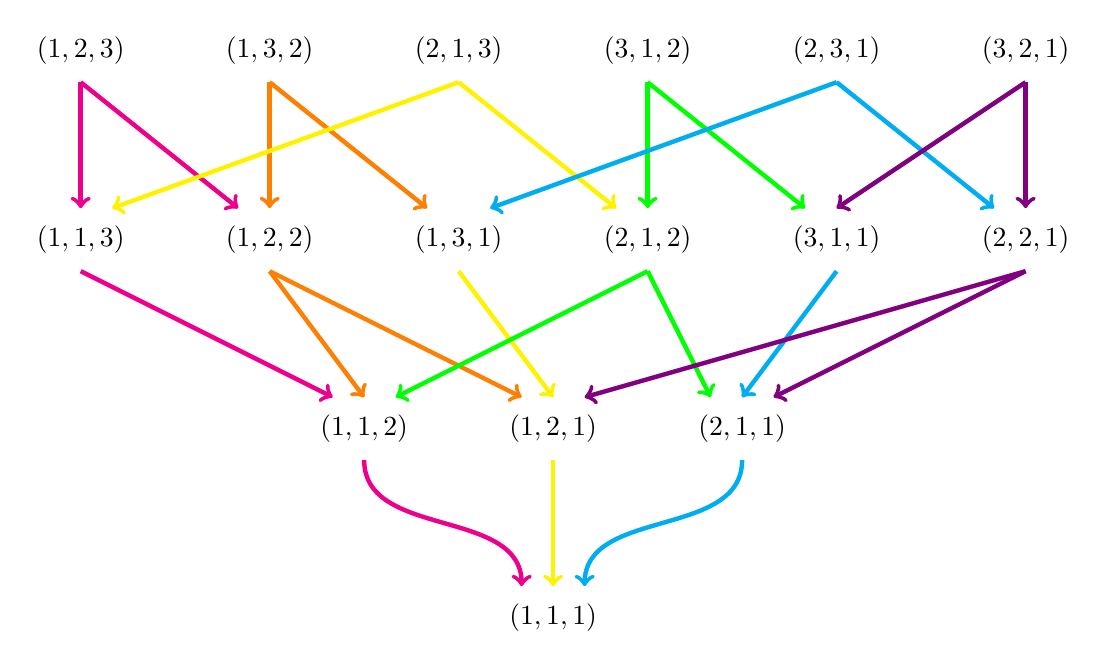
\begin{tikzpicture}[scale = 0.4]
            \node at (0,0) {$(1,1,1)$};

            \node at (-6,6) {$(1,1,2)$};                
            \node at (0,6)  {$(1,2,1)$};
            \node at (6,6)  {$(2,1,1)$};

            \node at (-15,12) {$(1,1,3)$};
            \node at (-9,12)  {$(1,2,2)$};
            \node at (-3,12)  {$(1,3,1)$};
            \node at (3,12)   {$(2,1,2)$};
            \node at (9,12)   {$(3,1,1)$};
            \node at (15,12)  {$(2,2,1)$};

            \node at (-15,18) {$(1,2,3)$};
            \node at (-9,18)  {$(1,3,2)$};
            \node at (-3,18)  {$(2,1,3)$};
            \node at (3,18)   {$(3,1,2)$};
            \node at (9,18)   {$(2,3,1)$};
            \node at (15,18)  {$(3,2,1)$};

            \draw [->][color=magenta, ultra thick]
                (-15,17) to (-15,13);
            \draw [->][color=magenta, ultra thick]
                (-15,17) to (-10,13);
            \draw [->][color=magenta, ultra thick]
                (-15,11) to (-7,7); 
            \draw [->][out=-90,in=90, ultra thick] 
                [color=magenta](-6,5) to (-1,1);

            \draw [->][color=brown!7!orange, ultra thick]
                (-9,17) to (-9,13);
            \draw [->][color=brown!7!orange, ultra thick]
                (-9,17) to (-4,13);
            \draw [->][color=brown!7!orange, ultra thick]
                (-9,11) to (-6,7);
            \draw [->][color=brown!7!orange, ultra thick]
                (-9,11) to (-1,7);

            \draw [->][color=yellow, ultra thick]
                (-3,17) to (-14,13);
            \draw [->][color=yellow, ultra thick]
                (-3,17) to (2,13);
            \draw [->][color=yellow, ultra thick]
                (-3,11) to (0,7); 
            \draw [->][out=-90,in=90, ultra thick] 
                [color=yellow](0,5) to (0,1);

            \draw [->][color = green,  ultra thick]
                (3,17) to (3,13);
            \draw [->][color=green, ultra thick]
                (3,17) to (8,13);
            \draw [->][color=green, ultra thick]
                (3,11) to (-5,7);
            \draw [->][color=green, ultra thick]
                (3,11) to (5,7);
        
            \draw [->][color=cyan, ultra thick]
                (9,17) to (-2,13);
            \draw [->][color=cyan, ultra thick]
                (9,17) to (14,13);
            \draw [->][color=cyan, ultra thick]
                (9,11) to (6,7); 
            \draw [->][out=-90,in=90, ultra thick] 
                [color=cyan](6,5) to (1,1);

            \draw [->][color=violet, ultra thick]
                (15,17) to (9,13);
            \draw [->][color=violet, ultra thick]
                (15,17) to (15,13);
            \draw [->][color=violet, ultra thick]
                (15,11) to (1,7);
            \draw [->][color=violet, ultra thick]
                (15,11) to (7,7);
        
        \end{tikzpicture}
        ~\\
        ~\\
        There are $4^2 = 16$ elements in this poset.
    \end{center}
\end{example}

\begin{rem}
    The two posets are isomorphic, and one can be obtained by
    applying the aforementioned bijection to the other.
\end{rem}

\chapter{The rational case}

For the whole chapter, we will consider 2 \emph{coprime}
integers $a$ and $b$ (meaning $a$ and $b$ have $1$ as their
greatest common divisor).

\section{Rational Parking Functions}

\begin{definition}[a, b - Parking Function]
    An \emph{a, b - parking function} is a sequence 
    $(a_1, a_2, \ldots, a_n)$ such that :\\
    \begin{itemize*}
        \item $n = a$\\
        \item its non-decreasing reordering 
        $(b_1, b_2, \ldots, b_n)$
        has $b_i \leqslant \frac{b}{a}(i-1) + 1$
        for all $i$.\\\\
    \end{itemize*}
    We denote by $\mathcal{PF}_{a,b}$ the set of 
    a, b - parking functions.
\end{definition}

\begin{example}
    ~\\
    \begin{itemize}
        \item Ex. 1 : $a > b$
            \subitem $a = 7$
            \subitem $b = 3$
            \subitem Limits of the non-decreasing
            reordering of any $f \in \mathcal{PF}_{7,3}$ :
            \subitem $[1,\ 1 \frac{3}{7},\ 1 \frac{6}{7},\ 
            2 \frac{2}{7},\ 2 \frac{5}{7},\ 3 \frac{1}{7},\ 
            3 \frac{4}{7}]$
            \subitem $f_1 = (2, 1, 1, 3, 2, 3, 1) \in
            \mathcal{PF}_{7,3}$
            \subitem $f_2 = (2, 1, 2, 3, 2, 3, 1) \notin
            \mathcal{PF}_{7,3}$, even though $f_2 \in
            \mathcal{PF}_7$
        \item Ex. 2 : $a < b$
            \subitem $a = 5$
            \subitem $b = 7$
            \subitem Limits of the non-decreasing            
            reordering of any $f \in \mathcal{PF}_{5,7}$ :
            \subitem $[1,\ 2 \frac{2}{5},\ 3 \frac{4}{5},\ 
            5 \frac{1}{5},\ 6 \frac{3}{5}]$
            \subitem $f_3 = (6, 3, 5, 1, 2) \in
            \mathcal{PF}_{5,7}$, even though $f_3 \notin
            \mathcal{PF}_5$
            \subitem $f_4 = (6, 3, 5, 1, 3) \notin
            \mathcal{PF}_{5,7}$\\
    \end{itemize}
\end{example}

\begin{theorem}
    Let $pf_{a,b}$ be the cardinal of $\mathcal{PF}_{a,b}$.
    We have $$pf_{a,b} = b^{a-1}$$
\end{theorem}

\begin{example}[$a = 3, b = 5$]
    ~\\
    \begin{itemize*}\\
        \item $pf_{a,b} = 25$
        \item Limits : $[1,\ 2 \frac{2}{3},\ 
            4 \frac{1}{3}]$\\\\
        \subitem $(1, 1, 1)$
        \subitem $(1, 1, 2)$
        \subitem $(1, 1, 3)$
        \subitem $(1, 1, 4)$
        \subitem $(1, 2, 1)$
        \subitem $(1, 2, 2)$
        \subitem $(1, 2, 3)$
        \subitem $(1, 2, 4)$
        \subitem $(1, 3, 1)$
        \subitem $(1, 3, 2)$
        \subitem $(1, 4, 1)$
        \subitem $(1, 4, 2)$
        \subitem $(2, 1, 1)$
        \subitem $(2, 1, 2)$
        \subitem $(2, 1, 3)$
        \subitem $(2, 1, 4)$
        \subitem $(2, 2, 1)$
        \subitem $(2, 3, 1)$
        \subitem $(2, 4, 1)$
        \subitem $(3, 1, 1)$
        \subitem $(3, 1, 2)$
        \subitem $(3, 2, 1)$
        \subitem $(4, 1, 1)$
        \subitem $(4, 1, 2)$
        \subitem $(4, 2, 1)$
    \end{itemize*}
\end{example}

\begin{rem}    
    $\mathcal{PF}_{n, n+1} = \mathcal{PF}_n$.
    In fact, we do have $b^{a-1} = (n+1)^{n-1}$.
\end{rem}

\subsection{Rational primitive parking functions}

\begin{definition}[Rational Primitive]
    A rational parking function $f$ is said
    \emph{primitive} if it is already in
    non-decreasing order.\\
    We denote by $\mathcal{PF'}_{a,b}$ the set of
    primitive a, b - parking functions.
\end{definition}

\begin{example}[$a = 4, b = 3$]
    Limits : $[1,\ 1 \frac{3}{4},\ 2 \frac{1}{2},\ 
    3 \frac{1}{4}]$
    \begin{align*}
        &f_1 = (1, 1, 2, 2) \in \mathcal{PF'}_{4,3}\\
        &f_2 = (1, 1, 2, 1) \notin \mathcal{PF'}_{4,3},
        \text{ even though } f_2 \in \mathcal{PF}_{4,3}.
    \end{align*}
\end{example}

\begin{theorem}
    Let $pf'_{a,b}$ be the cardinal of
    $\mathcal{PF'}_{a,b}$.
    We have $$\displaystyle pf'_{a,b} = 
    \frac{1}{a + b} \binom{a + b}{b}$$
    which is the \emph{rational Catalan number}
    $Cat(a,b)$.
\end{theorem}

\begin{example}[$a = 3, b = 5$]
    ~\\
    \begin{itemize*}
        \item $pf'_{a,b} = 7$
        \item Limits : $[1,\ 2 \frac{2}{3},\ 
            4 \frac{1}{3}]$\\\\
        \subitem $(1, 1, 1)$
        \subitem $(1, 1, 2)$
        \subitem $(1, 1, 3)$
        \subitem $(1, 1, 4)$
        \subitem $(1, 2, 2)$
        \subitem $(1, 2, 3)$
        \subitem $(1, 2, 4)$
    \end{itemize*}    
\end{example}

\begin{rem}
    $\mathcal{PF'}_{n,n+1} = \mathcal{PF'}_n$.
    In fact, we do have
    $$\frac{1}{n + n + 1} \binom{n + n + 1}{n + 1}
    = \frac{1}{2n + 1} \binom {2n + 1}{n + 1}
    = \frac{1}{2n + 1} \frac{(2n + 1)!}{n ! (n+1)!}$$
    $$= \frac{(2n)!}{n!(n+1)!}
    = \frac{1}{n+1} \frac{(2n)!}{n!n!}
    = \frac{1}{n+1} \binom{2n}{n}$$
\end{rem}

\section{Rational Non-crossing Partitions}

%maybe not those
%rational dyck paths
%rational labeled dyck paths
%examples of both
%covering relation on rational dyck paths
%covering relation on rational labeled dyck paths
%bijection between RDP and rational PPF
%bijection between RLDP and rational PF
%poset for RDP for a given n
%corresponding poset for rational PPF 
%poset for RLDP for a given n
%corresponding poset for rational PF

\begin{definition}[a, b - Non-crossing Partition]
    An \emph{a, b - non-crossing partition} is
    TODO\\
    We denote by $\mathcal{NC}_{a,b}$ the set of 
    a, b - non-crossing partitions.
\end{definition}

\begin{example}
    An abncp
\end{example}

\begin{theorem}
    Let $nc_{a,b}$ be the cardinal of $\mathcal{NC}_{a,b}$.
    We have $$nc_{a,b} = \frac{1}{a+b} \binom{a+b}{a} = 
    \frac{(a+b-1)!}{a!b!}$$, which is the rational Catalan
    number.
\end{theorem}

\begin{example}
    all abncp for some a b
\end{example}

\begin{prop}
    This means we can create a \emph{bijection} between
    $\mathcal{PF'}_{a,b}$ and $\mathcal{NC}_{a,b}$.
\end{prop}

\begin{proof}
    ~\\
\begin{itemize}
    \item $\mathcal{NC}_{a,b} \to \mathcal{PF'}_{a,b}$ :
    
    \item $\mathcal{PF'}_{a,b} \to \mathcal{NC}_{a,b}$ :
\end{itemize}
\end{proof}

\begin{definition}[a, b - Non-crossing 2-Partition]
    An \emph{a, b - Non-crossing 2-partition} is
    TODO\\
    We denote by $\mathcal{NC}^2_{a,b}$ the set of 
    a, b - non-crossing 2-partitions.
\end{definition}

\begin{example}
    some ncab2
\end{example}

\begin{theorem}
    Let $nc^2_{a,b}$ be the cardinal of $\mathcal{NC}^2_{a,b}$.
    We have $$nc^2_{a,b} = b^{a-1}$$.    
\end{theorem}

\begin{example}
    all ncab2 for some a b
\end{example}

\begin{prop}
    bijection
\end{prop}

\begin{proof}
    bijection proof
\end{proof}

\section{A direct poset linked to Rational Dyck paths}

\subsection{Rational Dyck Paths}

\begin{definition}[a, b - Dyck path]
    An \emph{a, b - Dyck word} is a word $w \in \{0,1\}^*$
    such that :
    \begin{itemize}
        \item for each \emph{suffix} $w'$ of $w$,
            $$|w'|_1 \geqslant \frac{a}{b}|w'|_0$$.
        \item $|w|_0 = b$.
        \item $|w|_1 = a$.
    \end{itemize}
    An a, b - Dyck word can be represented as a 
    \emph{path} from $(0,0)$ to $(b,a)$ that stays over
    $y = \frac{a}{b}x$, called an \emph{a, b - Dyck path} :
    \begin{itemize}
        \item Each $1$ corresponds to a \emph{North step}
        $\uparrow$. 
        \item Each $0$ corresponds to an \emph{East step}
        $\rightarrow$.
    \end{itemize}
    We denote by $\mathcal{R}_{a, b}$ the set of
    a, b - Dyck words.
\end{definition}

\begin{example}[$a > b : a = 7, b = 3$]
    ~\\
    \begin{align*}
        &w_1 = 1110011110 \text{ is \emph{not} a 7, 3 - Dyck
        word, because } |11100|_1 = 3\\
        & \hspace{5cm} < \frac{7}{3}|11100|_0
        = \frac{14}{3} = 4 \frac{1}{3}.\\
        &w_2 = 1110111010 \text{ \emph{is} a 7, 3 - Dyck 
        word : }\\
    \end{align*}
    \begin{center}
        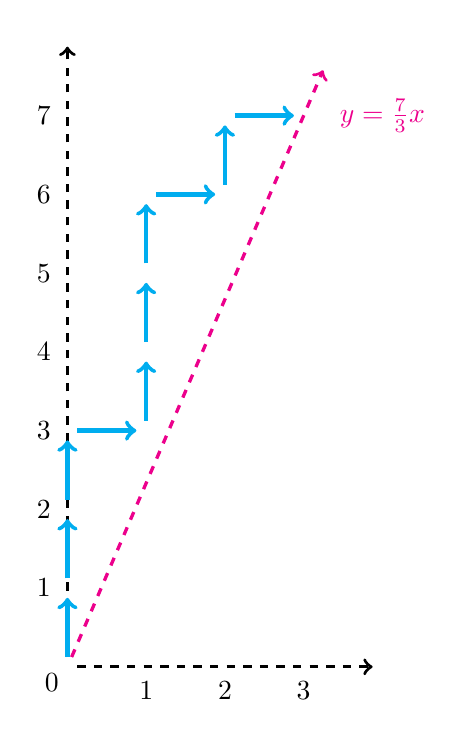
\begin{tikzpicture}[scale=1]
            \node (a) at (0, 0) {};
            \node (b) at (0, 8) {};
            \node (c) at (4, 0) {};
            \node (d) at (3.3, 7.7) {};
            \node (e) at (4, 7) [color = magenta]
                {$y = \frac{7}{3}x$}; 
            \draw [dashed, very thick, ->] (a) to (b);
            \draw [dashed, very thick, ->] (a) to (c);
            \draw [dashed, very thick, ->]
                [color = magenta] (a) to (d);

            \node (1)  at (0,0)   {};
            \node (2)  at (0,1)   {};
            \node (3)  at (0,2)   {};
            \node (4)  at (0,3)   {};
            \node (5)  at (1,3)   {};
            \node (6)  at (1,4)   {};
            \node (7)  at (1,5)   {};
            \node (8)  at (1,6)   {};
            \node (9)  at (2,6)   {};
            \node (10) at (2,7)   {};
            \node (11) at (3,7)   {};
            \draw [->, ultra thick, color = cyan]
                (1)  to (2);
            \draw [->, ultra thick, color = cyan] 
                (2)  to (3);
            \draw [->, ultra thick, color = cyan]
                (3)  to (4);
            \draw [->, ultra thick, color = cyan]
                (4)  to (5);
            \draw [->, ultra thick, color = cyan]
                (5)  to (6);
            \draw [->, ultra thick, color = cyan]
                (6)  to (7);
            \draw [->, ultra thick, color = cyan]
                (7)  to (8);
            \draw [->, ultra thick, color = cyan]
                (8)  to (9);
            \draw [->, ultra thick, color = cyan]
                (9)  to (10);
            \draw [->, ultra thick, color = cyan]
                (10) to (11);

            \node at (-0.2, -0.2) {$0$};
            \node at (-0.3, 1)    {$1$};
            \node at (1, -0.3)    {$1$};
            \node at (-0.3, 2)    {$2$};
            \node at (2, -0.3)    {$2$};
            \node at (-0.3, 3)    {$3$};
            \node at (3, -0.3)    {$3$};
            \node at (-0.3, 4)    {$4$};
            \node at (-0.3, 5)    {$5$};
            \node at (-0.3, 6)    {$6$};
            \node at (-0.3, 7)    {$7$};

        \end{tikzpicture}
    \end{center}
\end{example}

\begin{example}[$a < b : a = 3, b = 5$]
    ~\\
    \begin{align*}
        &w_1 = 10100010 \text{ is \emph{not} a 3, 5 - Dyck
        word, because } |101000|_1 = 2\\
        & \hspace{5cm} < \frac{3}{5}|101000|_0
        = \frac{12}{5} = 2 \frac{2}{5}.\\
        &w_2 = 10100100 \text{ \emph{is} a 3, 5 - Dyck 
        word : }\\
    \end{align*}
    \begin{center}
        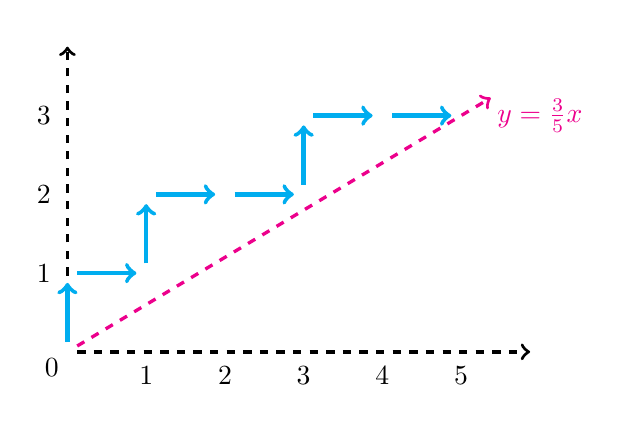
\begin{tikzpicture}[scale=1]
            \node (a) at (0, 0) {};
            \node (b) at (0, 4) {};
            \node (c) at (6, 0) {};
            \node (d) at (5.5, 3.3) {};
            \node (e) at (6, 3) [color = magenta]
                {$y = \frac{3}{5}x$}; 
            \draw [dashed, very thick, ->] (a) to (b);
            \draw [dashed, very thick, ->] (a) to (c);
            \draw [dashed, very thick, ->]
                [color = magenta] (a) to (d);

            \node (1)  at (0,0)   {};
            \node (2)  at (0,1)   {};
            \node (3)  at (1,1)   {};
            \node (4)  at (1,2)   {};
            \node (5)  at (2,2)   {};
            \node (6)  at (3,2)   {};
            \node (7)  at (3,3)   {};
            \node (8)  at (4,3)   {};
            \node (9)  at (5,3)   {};
            \draw [->, ultra thick, color = cyan]
                (1)  to (2);
            \draw [->, ultra thick, color = cyan] 
                (2)  to (3);
            \draw [->, ultra thick, color = cyan]
                (3)  to (4);
            \draw [->, ultra thick, color = cyan]
                (4)  to (5);
            \draw [->, ultra thick, color = cyan]
                (5)  to (6);
            \draw [->, ultra thick, color = cyan]
                (6)  to (7);
            \draw [->, ultra thick, color = cyan]
                (7)  to (8);
            \draw [->, ultra thick, color = cyan]
                (8)  to (9);

            \node at (-0.2, -0.2) {$0$};
            \node at (-0.3, 1)    {$1$};
            \node at (1, -0.3)    {$1$};
            \node at (-0.3, 2)    {$2$};
            \node at (2, -0.3)    {$2$};
            \node at (-0.3, 3)    {$3$};
            \node at (3, -0.3)    {$3$};
            \node at (4, -0.3)    {$4$};
            \node at (5, -0.3)    {$5$};

        \end{tikzpicture}
    \end{center}
\end{example}

\begin{theorem}
    Let $r_{a,b}$ be the cardinal of $\mathcal{R}_{a,b}$.
    We have $$r_{a,b} = \frac{1}{a+b} \binom {a+b}{a} =
    \frac{(a+b-1)!}{a!b!}$$, which is again the rational
    Catalan number.
\end{theorem}

\begin{example}[$a = 7, b = 2$]
    $r_n = 4$.
    \begin{center}
        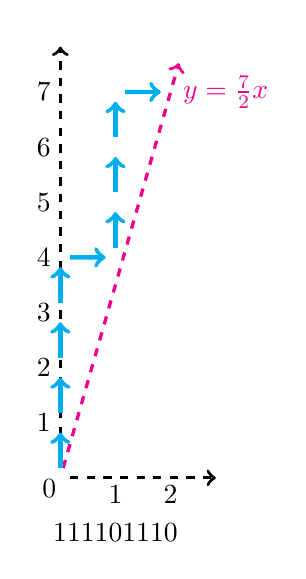
\begin{tikzpicture}[scale = 0.7]
            \node (a) at (0, 0) {};
            \node (b) at (0, 8) {};
            \node (c) at (3, 0) {};
            \node (d) at (2.2, 7.7) {};
            \node (e) at (3, 7) [color = magenta]
                {$y = \frac{7}{2}x$}; 
            \draw [dashed, very thick, ->] (a) to (b);
            \draw [dashed, very thick, ->] (a) to (c);
            \draw [dashed, very thick, ->]
                [color = magenta] (a) to (d);

            \node (1)  at (0,0)   {};
            \node (2)  at (0,1)   {};
            \node (3)  at (0,2)   {};
            \node (4)  at (0,3)   {};
            \node (5)  at (0,4)   {};
            \node (6)  at (1,4)   {};
            \node (7)  at (1,5)   {};
            \node (8)  at (1,6)   {};
            \node (9)  at (1,7)   {};
            \node (10) at (2,7)   {};
            \draw [->, ultra thick, color = cyan]
                (1)  to (2);
            \draw [->, ultra thick, color = cyan] 
                (2)  to (3);
            \draw [->, ultra thick, color = cyan]
                (3)  to (4);
            \draw [->, ultra thick, color = cyan]
                (4)  to (5);
            \draw [->, ultra thick, color = cyan]
                (5)  to (6);
            \draw [->, ultra thick, color = cyan]
                (6)  to (7);
            \draw [->, ultra thick, color = cyan]
                (7)  to (8);
            \draw [->, ultra thick, color = cyan]
                (8)  to (9);
            \draw [->, ultra thick, color = cyan]
                (9)  to (10);

            \node at (-0.2, -0.2) {$0$};
            \node at (-0.3, 1)    {$1$};
            \node at (1, -0.3)    {$1$};
            \node at (-0.3, 2)    {$2$};
            \node at (2, -0.3)    {$2$};
            \node at (-0.3, 3)    {$3$};
            \node at (-0.3, 4)    {$4$};
            \node at (-0.3, 5)    {$5$};
            \node at (-0.3, 6)    {$6$};
            \node at (-0.3, 7)    {$7$};
            \node at (1, -1)      {$111101110$};

        \end{tikzpicture}
        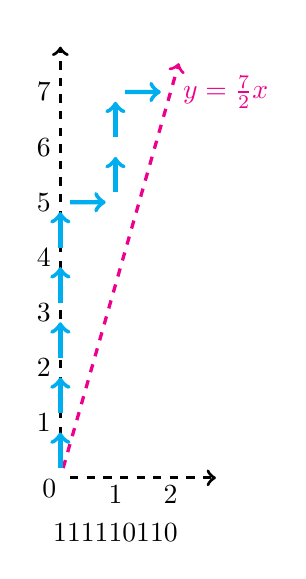
\begin{tikzpicture}[scale = 0.7]
            \node (a) at (0, 0) {};
            \node (b) at (0, 8) {};
            \node (c) at (3, 0) {};
            \node (d) at (2.2, 7.7) {};
            \node (e) at (3, 7) [color = magenta]
                {$y = \frac{7}{2}x$}; 
            \draw [dashed, very thick, ->] (a) to (b);
            \draw [dashed, very thick, ->] (a) to (c);
            \draw [dashed, very thick, ->]
                [color = magenta] (a) to (d);

            \node (1)  at (0,0)   {};
            \node (2)  at (0,1)   {};
            \node (3)  at (0,2)   {};
            \node (4)  at (0,3)   {};
            \node (5)  at (0,4)   {};
            \node (6)  at (0,5)   {};
            \node (7)  at (1,5)   {};
            \node (8)  at (1,6)   {};
            \node (9)  at (1,7)   {};
            \node (10) at (2,7)   {};
            \draw [->, ultra thick, color = cyan]
                (1)  to (2);
            \draw [->, ultra thick, color = cyan] 
                (2)  to (3);
            \draw [->, ultra thick, color = cyan]
                (3)  to (4);
            \draw [->, ultra thick, color = cyan]
                (4)  to (5);
            \draw [->, ultra thick, color = cyan]
                (5)  to (6);
            \draw [->, ultra thick, color = cyan]
                (6)  to (7);
            \draw [->, ultra thick, color = cyan]
                (7)  to (8);
            \draw [->, ultra thick, color = cyan]
                (8)  to (9);
            \draw [->, ultra thick, color = cyan]
                (9)  to (10);

            \node at (-0.2, -0.2) {$0$};
            \node at (-0.3, 1)    {$1$};
            \node at (1, -0.3)    {$1$};
            \node at (-0.3, 2)    {$2$};
            \node at (2, -0.3)    {$2$};
            \node at (-0.3, 3)    {$3$};
            \node at (-0.3, 4)    {$4$};
            \node at (-0.3, 5)    {$5$};
            \node at (-0.3, 6)    {$6$};
            \node at (-0.3, 7)    {$7$};
            \node at (1, -1)      {$111110110$};

        \end{tikzpicture}
        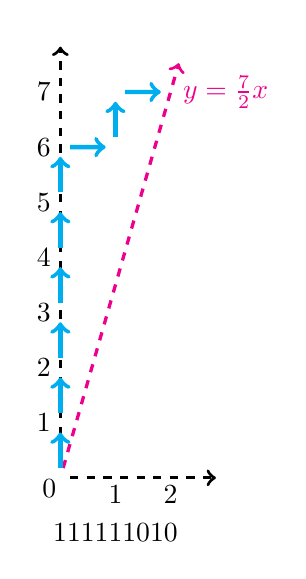
\begin{tikzpicture}[scale = 0.7]
            \node (a) at (0, 0) {};
            \node (b) at (0, 8) {};
            \node (c) at (3, 0) {};
            \node (d) at (2.2, 7.7) {};
            \node (e) at (3, 7) [color = magenta]
                {$y = \frac{7}{2}x$}; 
            \draw [dashed, very thick, ->] (a) to (b);
            \draw [dashed, very thick, ->] (a) to (c);
            \draw [dashed, very thick, ->]
                [color = magenta] (a) to (d);

            \node (1)  at (0,0)   {};
            \node (2)  at (0,1)   {};
            \node (3)  at (0,2)   {};
            \node (4)  at (0,3)   {};
            \node (5)  at (0,4)   {};
            \node (6)  at (0,5)   {};
            \node (7)  at (0,6)   {};
            \node (8)  at (1,6)   {};
            \node (9)  at (1,7)   {};
            \node (10) at (2,7)   {};
            \draw [->, ultra thick, color = cyan]
                (1)  to (2);
            \draw [->, ultra thick, color = cyan] 
                (2)  to (3);
            \draw [->, ultra thick, color = cyan]
                (3)  to (4);
            \draw [->, ultra thick, color = cyan]
                (4)  to (5);
            \draw [->, ultra thick, color = cyan]
                (5)  to (6);
            \draw [->, ultra thick, color = cyan]
                (6)  to (7);
            \draw [->, ultra thick, color = cyan]
                (7)  to (8);
            \draw [->, ultra thick, color = cyan]
                (8)  to (9);
            \draw [->, ultra thick, color = cyan]
                (9)  to (10);

            \node at (-0.2, -0.2) {$0$};
            \node at (-0.3, 1)    {$1$};
            \node at (1, -0.3)    {$1$};
            \node at (-0.3, 2)    {$2$};
            \node at (2, -0.3)    {$2$};
            \node at (-0.3, 3)    {$3$};
            \node at (-0.3, 4)    {$4$};
            \node at (-0.3, 5)    {$5$};
            \node at (-0.3, 6)    {$6$};
            \node at (-0.3, 7)    {$7$};
            \node at (1, -1)      {$111111010$};

        \end{tikzpicture}
        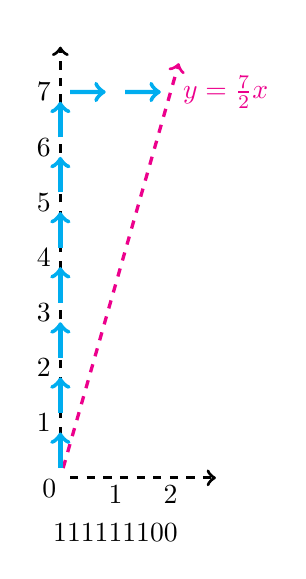
\begin{tikzpicture}[scale = 0.7]
            \node (a) at (0, 0) {};
            \node (b) at (0, 8) {};
            \node (c) at (3, 0) {};
            \node (d) at (2.2, 7.7) {};
            \node (e) at (3, 7) [color = magenta]
                {$y = \frac{7}{2}x$}; 
            \draw [dashed, very thick, ->] (a) to (b);
            \draw [dashed, very thick, ->] (a) to (c);
            \draw [dashed, very thick, ->]
                [color = magenta] (a) to (d);

            \node (1)  at (0,0)   {};
            \node (2)  at (0,1)   {};
            \node (3)  at (0,2)   {};
            \node (4)  at (0,3)   {};
            \node (5)  at (0,4)   {};
            \node (6)  at (0,5)   {};
            \node (7)  at (0,6)   {};
            \node (8)  at (0,7)   {};
            \node (9)  at (1,7)   {};
            \node (10) at (2,7)   {};
            \draw [->, ultra thick, color = cyan]
                (1)  to (2);
            \draw [->, ultra thick, color = cyan] 
                (2)  to (3);
            \draw [->, ultra thick, color = cyan]
                (3)  to (4);
            \draw [->, ultra thick, color = cyan]
                (4)  to (5);
            \draw [->, ultra thick, color = cyan]
                (5)  to (6);
            \draw [->, ultra thick, color = cyan]
                (6)  to (7);
            \draw [->, ultra thick, color = cyan]
                (7)  to (8);
            \draw [->, ultra thick, color = cyan]
                (8)  to (9);
            \draw [->, ultra thick, color = cyan]
                (9)  to (10);

            \node at (-0.2, -0.2) {$0$};
            \node at (-0.3, 1)    {$1$};
            \node at (1, -0.3)    {$1$};
            \node at (-0.3, 2)    {$2$};
            \node at (2, -0.3)    {$2$};
            \node at (-0.3, 3)    {$3$};
            \node at (-0.3, 4)    {$4$};
            \node at (-0.3, 5)    {$5$};
            \node at (-0.3, 6)    {$6$};
            \node at (-0.3, 7)    {$7$};
            \node at (1, -1)      {$111111100$};

        \end{tikzpicture}
    \end{center}
\end{example}

\begin{prop}
    This means we can create a \emph{bijection} between
    $\mathcal{PF'}_{a,b}$ and $\mathcal{R}_{a,b}$.
\end{prop}

\begin{proof}
    ~\
\begin{itemize}
    \item $\mathcal{PF'}_{a,b} \to \mathcal{R}_{a,b}$ :
    Let $f = (a_1, \ldots, a_n) \in \mathcal{PF'}_{a,b}$
    be our rational primitive parking function.
    For $i \in \{1, \ldots, b\}$, we define $l_i$ the
    number of occurences of $i$ in $f$.\\
    The corresponding rational Dyck word will be
    $\underbrace{1 \cdots 1}_{l_1}0
     \underbrace{1 \cdots 1}_{l_2}0 \cdots
     \underbrace{1 \cdots 1}_{l_b}0$.
    
    \item $\mathcal{R}_{a,b} \to \mathcal{PF'}_{a,b}$ :
    Let $w$ be our rational Dyck word, and consider its path
    representation. We define $s_i$ to be the distance
    between the segment from $(0, i - 1)$ to $(0, i)$
    and the $i^{th}$ North step. Then, let $a_i = s_i + 1$.\\
    The corresponding rational primitive parking function is 
    $(a_1, \ldots, a_a)$.
\end{itemize}
\end{proof}

\begin{rem}
    This bijection is exactly the same as the one between
    classical primitive parking functions and Dyck paths.
\end{rem}

\begin{example}[$a > b : a = 7, b = 3,
    \mathcal{PF'}_{a,b} \to \mathcal{R}_{a,b}$]
    ~\
    \begin{itemize}
        \item $f = (1, 1, 1, 2, 2, 3, 3)$
            \subitem $l_1 = 3$
            \hspace{2cm} $l_2 = 2$
            \hspace{2cm} $l_3 = 2$
        \item $w = (1110110110)$
    \end{itemize}

    \begin{center}
        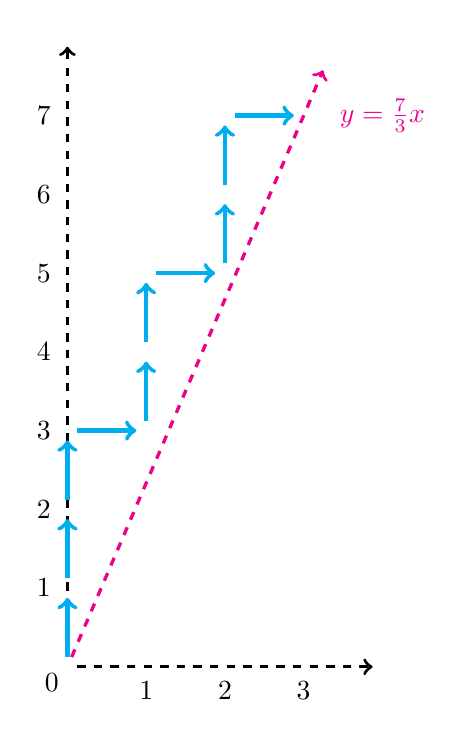
\begin{tikzpicture}[scale=1]
            \node (a) at (0, 0) {};
            \node (b) at (0, 8) {};
            \node (c) at (4, 0) {};
            \node (d) at (3.3, 7.7) {};
            \node (e) at (4, 7) [color = magenta]
                {$y = \frac{7}{3}x$}; 
            \draw [dashed, very thick, ->] (a) to (b);
            \draw [dashed, very thick, ->] (a) to (c);
            \draw [dashed, very thick, ->]
                [color = magenta] (a) to (d);

            \node (1)  at (0,0)   {};
            \node (2)  at (0,1)   {};
            \node (3)  at (0,2)   {};
            \node (4)  at (0,3)   {};
            \node (5)  at (1,3)   {};
            \node (6)  at (1,4)   {};
            \node (7)  at (1,5)   {};
            \node (8)  at (2,5)   {};
            \node (9)  at (2,6)   {};
            \node (10) at (2,7)   {};
            \node (11) at (3,7)   {};
            \draw [->, ultra thick, color = cyan]
                (1)  to (2);
            \draw [->, ultra thick, color = cyan] 
                (2)  to (3);
            \draw [->, ultra thick, color = cyan]
                (3)  to (4);
            \draw [->, ultra thick, color = cyan]
                (4)  to (5);
            \draw [->, ultra thick, color = cyan]
                (5)  to (6);
            \draw [->, ultra thick, color = cyan]
                (6)  to (7);
            \draw [->, ultra thick, color = cyan]
                (7)  to (8);
            \draw [->, ultra thick, color = cyan]
                (8)  to (9);
            \draw [->, ultra thick, color = cyan]
                (9)  to (10);
            \draw [->, ultra thick, color = cyan]
                (10) to (11);

            \node at (-0.2, -0.2) {$0$};
            \node at (-0.3, 1)    {$1$};
            \node at (1, -0.3)    {$1$};
            \node at (-0.3, 2)    {$2$};
            \node at (2, -0.3)    {$2$};
            \node at (-0.3, 3)    {$3$};
            \node at (3, -0.3)    {$3$};
            \node at (-0.3, 4)    {$4$};
            \node at (-0.3, 5)    {$5$};
            \node at (-0.3, 6)    {$6$};
            \node at (-0.3, 7)    {$7$};
        \end{tikzpicture}
    \end{center}
\end{example}

\begin{example}[$a < b : a = 3, b = 5,
    \mathcal{PF'}_{a,b} \to \mathcal{R}_{a,b}$]
    ~\
    \begin{itemize}
        \item $f = (1, 1, 4)$
            \subitem $l_1 = 2$
            \hspace{2cm} $l_2$
            \hspace{2cm} $l_3 = 0$
            \subitem $l_4 = 1$
            \hspace{2cm} $l_5 = 0$
        \item $w = 11000100$
    \end{itemize}

    \begin{center}
        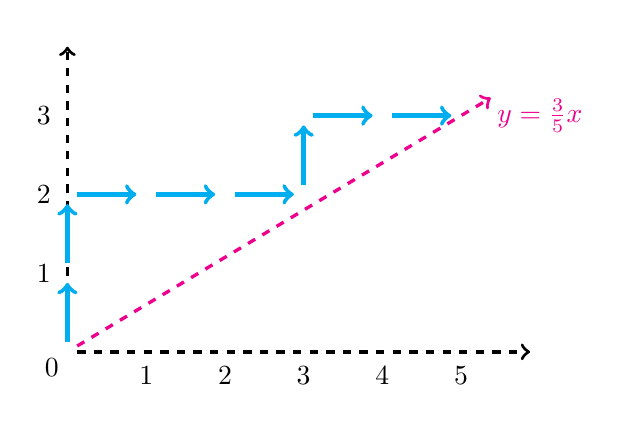
\begin{tikzpicture}[scale=1]
            \node (a) at (0, 0) {};
            \node (b) at (0, 4) {};
            \node (c) at (6, 0) {};
            \node (d) at (5.5, 3.3) {};
            \node (e) at (6, 3) [color = magenta]
                {$y = \frac{3}{5}x$}; 
            \draw [dashed, very thick, ->] (a) to (b);
            \draw [dashed, very thick, ->] (a) to (c);
            \draw [dashed, very thick, ->]
                [color = magenta] (a) to (d);

            \node (1)  at (0,0)   {};
            \node (2)  at (0,1)   {};
            \node (3)  at (0,2)   {};
            \node (4)  at (1,2)   {};
            \node (5)  at (2,2)   {};
            \node (6)  at (3,2)   {};
            \node (7)  at (3,3)   {};
            \node (8)  at (4,3)   {};
            \node (9)  at (5,3)   {};
            \draw [->, ultra thick, color = cyan]
                (1)  to (2);
            \draw [->, ultra thick, color = cyan] 
                (2)  to (3);
            \draw [->, ultra thick, color = cyan]
                (3)  to (4);
            \draw [->, ultra thick, color = cyan]
                (4)  to (5);
            \draw [->, ultra thick, color = cyan]
                (5)  to (6);
            \draw [->, ultra thick, color = cyan]
                (6)  to (7);
            \draw [->, ultra thick, color = cyan]
                (7)  to (8);
            \draw [->, ultra thick, color = cyan]
                (8)  to (9);

            \node at (-0.2, -0.2) {$0$};
            \node at (-0.3, 1)    {$1$};
            \node at (1, -0.3)    {$1$};
            \node at (-0.3, 2)    {$2$};
            \node at (2, -0.3)    {$2$};
            \node at (-0.3, 3)    {$3$};
            \node at (3, -0.3)    {$3$};
            \node at (4, -0.3)    {$4$};
            \node at (5, -0.3)    {$5$};
        \end{tikzpicture}
    \end{center}
\end{example}

\begin{example}[$a > b : a = 7, b = 3,
    \mathcal{R}_{a,b} \to \mathcal{PF'}_{a,b}$]
    ~\
    \begin{itemize}
        \item $w = 1111011010$
    \end{itemize}

    \begin{center}
        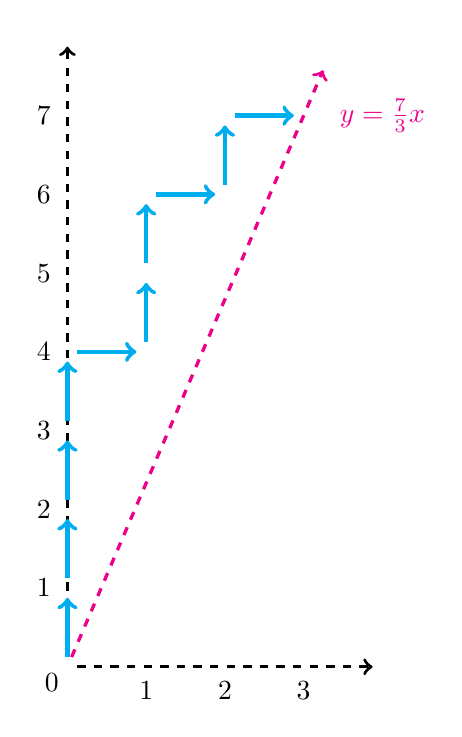
\begin{tikzpicture}[scale=1]
            \node (a) at (0, 0) {};
            \node (b) at (0, 8) {};
            \node (c) at (4, 0) {};
            \node (d) at (3.3, 7.7) {};
            \node (e) at (4, 7) [color = magenta]
                {$y = \frac{7}{3}x$}; 
            \draw [dashed, very thick, ->] (a) to (b);
            \draw [dashed, very thick, ->] (a) to (c);
            \draw [dashed, very thick, ->]
                [color = magenta] (a) to (d);

            \node (1)  at (0,0)   {};
            \node (2)  at (0,1)   {};
            \node (3)  at (0,2)   {};
            \node (4)  at (0,3)   {};
            \node (5)  at (0,4)   {};
            \node (6)  at (1,4)   {};
            \node (7)  at (1,5)   {};
            \node (8)  at (1,6)   {};
            \node (9)  at (2,6)   {};
            \node (10) at (2,7)   {};
            \node (11) at (3,7)   {};
            \draw [->, ultra thick, color = cyan]
                (1)  to (2);
            \draw [->, ultra thick, color = cyan] 
                (2)  to (3);
            \draw [->, ultra thick, color = cyan]
                (3)  to (4);
            \draw [->, ultra thick, color = cyan]
                (4)  to (5);
            \draw [->, ultra thick, color = cyan]
                (5)  to (6);
            \draw [->, ultra thick, color = cyan]
                (6)  to (7);
            \draw [->, ultra thick, color = cyan]
                (7)  to (8);
            \draw [->, ultra thick, color = cyan]
                (8)  to (9);
            \draw [->, ultra thick, color = cyan]
                (9)  to (10);
            \draw [->, ultra thick, color = cyan]
                (10) to (11);

            \node at (-0.2, -0.2) {$0$};
            \node at (-0.3, 1)    {$1$};
            \node at (1, -0.3)    {$1$};
            \node at (-0.3, 2)    {$2$};
            \node at (2, -0.3)    {$2$};
            \node at (-0.3, 3)    {$3$};
            \node at (3, -0.3)    {$3$};
            \node at (-0.3, 4)    {$4$};
            \node at (-0.3, 5)    {$5$};
            \node at (-0.3, 6)    {$6$};
            \node at (-0.3, 7)    {$7$};

        \end{tikzpicture}
    \end{center}
    \begin{itemize}
        \item Distances : 
            \subitem $s_1 = 0$
                \hspace{2cm} $a_1 = 1$
            \subitem $s_2 = 0$
                \hspace{2cm} $a_2 = 1$
            \subitem $s_3 = 0$
                \hspace{2cm} $a_3 = 1$
            \subitem $s_4 = 0$
                \hspace{2cm} $a_4 = 1$
            \subitem $s_5 = 1$
                \hspace{2cm} $a_5 = 2$
            \subitem $s_6 = 1$
                \hspace{2cm} $a_6 = 2$
            \subitem $s_7 = 2$
                \hspace{2cm} $a_7 = 3$
        \item $f = (1, 1, 1, 1, 2, 2, 3)$
    \end{itemize}
    
\end{example}

\begin{example}[$a < b : a = 3, b = 5,
    \mathcal{R}_{a,b} \to \mathcal{PF'}_{a,b}$]
    ~\
    \begin{itemize}
        \item $w = 10101000$
    \end{itemize}

    \begin{center}
        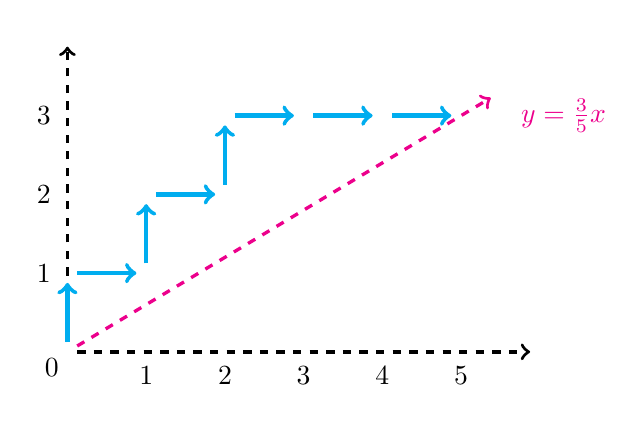
\begin{tikzpicture}[scale=1]
            \node (a) at (0, 0) {};
            \node (b) at (0, 4) {};
            \node (c) at (6, 0) {};
            \node (d) at (5.5, 3.3) {};
            \node (e) at (6.3, 3) [color = magenta]
                {$y = \frac{3}{5}x$}; 
            \draw [dashed, very thick, ->] (a) to (b);
            \draw [dashed, very thick, ->] (a) to (c);
            \draw [dashed, very thick, ->]
                [color = magenta] (a) to (d);

            \node (1)  at (0,0)   {};
            \node (2)  at (0,1)   {};
            \node (3)  at (1,1)   {};
            \node (4)  at (1,2)   {};
            \node (5)  at (2,2)   {};
            \node (6)  at (2,3)   {};
            \node (7)  at (3,3)   {};
            \node (8)  at (4,3)   {};
            \node (9)  at (5,3)   {};
            \draw [->, ultra thick, color = cyan]
                (1)  to (2);
            \draw [->, ultra thick, color = cyan] 
                (2)  to (3);
            \draw [->, ultra thick, color = cyan]
                (3)  to (4);
            \draw [->, ultra thick, color = cyan]
                (4)  to (5);
            \draw [->, ultra thick, color = cyan]
                (5)  to (6);
            \draw [->, ultra thick, color = cyan]
                (6)  to (7);
            \draw [->, ultra thick, color = cyan]
                (7)  to (8);
            \draw [->, ultra thick, color = cyan]
                (8)  to (9);

            \node at (-0.2, -0.2) {$0$};
            \node at (-0.3, 1)    {$1$};
            \node at (1, -0.3)    {$1$};
            \node at (-0.3, 2)    {$2$};
            \node at (2, -0.3)    {$2$};
            \node at (-0.3, 3)    {$3$};
            \node at (3, -0.3)    {$3$};
            \node at (4, -0.3)    {$4$};
            \node at (5, -0.3)    {$5$};

        \end{tikzpicture}
    \end{center}
    \begin{itemize}
        \item Distances : 
            \subitem $s_1 = 0$
                \hspace{2cm} $a_1 = 1$
            \subitem $s_2 = 1$
                \hspace{2cm} $a_2 = 2$
            \subitem $s_3 = 2$
                \hspace{2cm} $a_3 = 3$
        \item $f = (1, 2, 3)$
    \end{itemize}
    
\end{example}

\subsection{Rational Labeled Dyck Paths}

\begin{definition}[Labeled a, b - Dyck Path]
    A \emph{labeled a, b - Dyck word} is a word $w \in 
    \{0, \ldots, n\}^*$ such that :
    \begin{itemize}
        \item for each suffix $w'$ of $w$,
            $$|w'|_{\neq 0} \geqslant \frac{a}{b}|w'|_0$$.
        \item $|w|_0 = b$.
        \item $|w|_{\neq 0} = a$.
        \item for each $i \in \{1, \ldots, a\}$, $w$ has 
            exactly one occurence of $i$.
        \item if $w_i \neq 0$ and $w_{i+1} \neq 0$,
            then $w_i < w_{i+1}$. That is, consecutive
            North steps have increasing labels.
    \end{itemize}
    A labeled a, b - Dyck word can be represented
    as a path from $(0,0)$ to $(b,a)$, where each North
    step is associated to a label :
    \begin{itemize}
        \item Each $i \neq 0$ corresponds to a
            \emph{North step} $\uparrow$ labeled $i$.
        \item Each $0$ corresponds to an
            \emph{East step} $\rightarrow$.
    \end{itemize}
    Those paths are called \emph{labeled a, b - Dyck paths}.\\
    We denote by $\mathcal{LR}_{a,b}$ the set of labeled
    a, b - Dyck words.
\end{definition}

\begin{example}[$a > b : a = 7, b = 3$]
       $w_2 = 2456017030$ :\\
    \begin{center}
        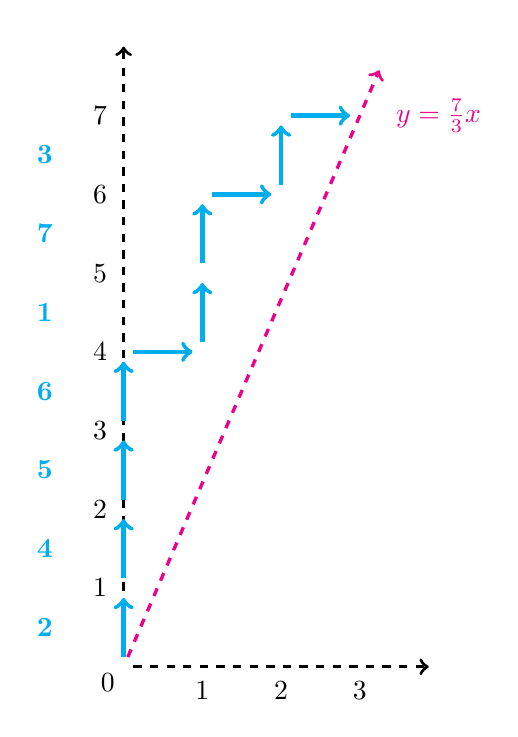
\begin{tikzpicture}[scale=1]
            \node (a) at (0, 0) {};
            \node (b) at (0, 8) {};
            \node (c) at (4, 0) {};
            \node (d) at (3.3, 7.7) {};
            \node (e) at (4, 7) [color = magenta]
                {$y = \frac{7}{3}x$}; 
            \draw [dashed, very thick, ->] (a) to (b);
            \draw [dashed, very thick, ->] (a) to (c);
            \draw [dashed, very thick, ->]
                [color = magenta] (a) to (d);

            \node (1)  at (0,0)   {};
            \node (2)  at (0,1)   {};
            \node (3)  at (0,2)   {};
            \node (4)  at (0,3)   {};
            \node (5)  at (0,4)   {};
            \node (6)  at (1,4)   {};
            \node (7)  at (1,5)   {};
            \node (8)  at (1,6)   {};
            \node (9)  at (2,6)   {};
            \node (10) at (2,7)   {};
            \node (11) at (3,7)   {};
            \draw [->, ultra thick, color = cyan]
                (1)  to (2);
            \draw [->, ultra thick, color = cyan] 
                (2)  to (3);
            \draw [->, ultra thick, color = cyan]
                (3)  to (4);
            \draw [->, ultra thick, color = cyan]
                (4)  to (5);
            \draw [->, ultra thick, color = cyan]
                (5)  to (6);
            \draw [->, ultra thick, color = cyan]
                (6)  to (7);
            \draw [->, ultra thick, color = cyan]
                (7)  to (8);
            \draw [->, ultra thick, color = cyan]
                (8)  to (9);
            \draw [->, ultra thick, color = cyan]
                (9)  to (10);
            \draw [->, ultra thick, color = cyan]
                (10) to (11);

            \node at (-0.2, -0.2) {$0$};
            \node at (-0.3, 1)    {$1$};
            \node at (1, -0.3)    {$1$};
            \node at (-0.3, 2)    {$2$};
            \node at (2, -0.3)    {$2$};
            \node at (-0.3, 3)    {$3$};
            \node at (3, -0.3)    {$3$};
            \node at (-0.3, 4)    {$4$};
            \node at (-0.3, 5)    {$5$};
            \node at (-0.3, 6)    {$6$};
            \node at (-0.3, 7)    {$7$};

            \node [color = cyan] at (-1, 0.5) {\textbf{2}};
            \node [color = cyan] at (-1, 1.5) {\textbf{4}};
            \node [color = cyan] at (-1, 2.5) {\textbf{5}};
            \node [color = cyan] at (-1, 3.5) {\textbf{6}};
            \node [color = cyan] at (-1, 4.5) {\textbf{1}};
            \node [color = cyan] at (-1, 5.5) {\textbf{7}};
            \node [color = cyan] at (-1, 6.5) {\textbf{3}};
        \end{tikzpicture}
    \end{center}
\end{example}

\begin{example}[$a < b : a = 3, b = 5$]
    $w = 20130000$ :\\
 \begin{center}
     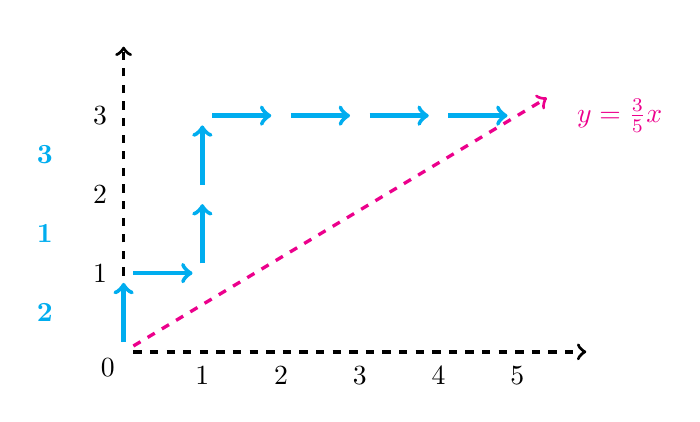
\begin{tikzpicture}[scale=1]
         \node (a) at (0, 0) {};
         \node (b) at (0, 4) {};
         \node (c) at (6, 0) {};
         \node (d) at (5.5, 3.3) {};
         \node (e) at (6.3, 3) [color = magenta]
             {$y = \frac{3}{5}x$}; 
         \draw [dashed, very thick, ->] (a) to (b);
         \draw [dashed, very thick, ->] (a) to (c);
         \draw [dashed, very thick, ->]
             [color = magenta] (a) to (d);

         \node (1)  at (0,0)   {};
         \node (2)  at (0,1)   {};
         \node (3)  at (1,1)   {};
         \node (4)  at (1,2)   {};
         \node (5)  at (1,3)   {};
         \node (6)  at (2,3)   {};
         \node (7)  at (3,3)   {};
         \node (8)  at (4,3)   {};
         \node (9)  at (5,3)   {};
         \draw [->, ultra thick, color = cyan]
             (1)  to (2);
         \draw [->, ultra thick, color = cyan] 
             (2)  to (3);
         \draw [->, ultra thick, color = cyan]
             (3)  to (4);
         \draw [->, ultra thick, color = cyan]
             (4)  to (5);
         \draw [->, ultra thick, color = cyan]
             (5)  to (6);
         \draw [->, ultra thick, color = cyan]
             (6)  to (7);
         \draw [->, ultra thick, color = cyan]
             (7)  to (8);
         \draw [->, ultra thick, color = cyan]
             (8)  to (9);

         \node at (-0.2, -0.2) {$0$};
         \node at (-0.3, 1)    {$1$};
         \node at (1, -0.3)    {$1$};
         \node at (-0.3, 2)    {$2$};
         \node at (2, -0.3)    {$2$};
         \node at (-0.3, 3)    {$3$};
         \node at (3, -0.3)    {$3$};
         \node at (4, -0.3)    {$4$};
         \node at (5, -0.3)    {$5$};

         \node [color = cyan] at (-1, 0.5) {\textbf{2}};
         \node [color = cyan] at (-1, 1.5) {\textbf{1}};
         \node [color = cyan] at (-1, 2.5) {\textbf{3}};
     \end{tikzpicture}
 \end{center}
\end{example}

\begin{theorem}
    Let $lr_{a,b}$ be the cardinal of $\mathcal{LR}_{a,b}$.
    We have $$lr_{a,b} = b^{a - 1}$$.
\end{theorem}

\begin{example}[$a > b : a = 4, b = 3$]
    $lr_{a,b} = 3^3 = 27$
    \begin{itemize}
        \item Word of shape $XXXX000$ :
            \subitem $1234000$
        \item Words of shape $XXX0X00$ :
            \subitem $1230400$
            \hspace{2cm} $1240300$
            \hspace{2cm} $1340200$
            \subitem $2340100$
        \item Words of shape $XX0XX00$ :
            \subitem $1203400$
            \hspace{2cm} $1302400$
            \hspace{2cm} $1402300$
            \subitem $2301400$
            \hspace{2cm} $2401300$
            \hspace{2cm} $3401200$
        \item Words of shape $XXX00X0$ :
            \subitem $1230040$
            \hspace{2cm} $1240030$
            \hspace{2cm} $1340020$
            \subitem $2340010$
        \item Words of shape $XX0X0X0$ :
            \subitem $1203040$
            \hspace{2cm} $1204030$
            \hspace{2cm} $1302040$
            \subitem $1304020$
            \hspace{2cm} $1402030$
            \hspace{2cm} $1403020$
            \subitem $2301040$
            \hspace{2cm} $2304010$
            \hspace{2cm} $2401030$
            \subitem $2403010$
            \hspace{2cm} $3401020$
            \hspace{2cm} $3402010$
    \end{itemize}
    
\end{example}

\begin{prop}
    This means we can create a \emph{bijection} between
    $\mathcal{PF}_{a,b}$ and $\mathcal{LR}_{a,b}$.
\end{prop}

\begin{proof}
    ~\
    \begin{itemize}
        \item $\mathcal{PF}_{a,b} \to \mathcal{LR}_{a,b}$ :
        Let $f = (a_1, \ldots, a_n) \in \mathcal{PF}_{a,b}$
        be our a, b - parking function. For $i \in \{1, \ldots,
        b\}$, we define $im_i$ : $\{j\ |\ a_j = i\}$. \\
        We then define $im_{i,1}, \ldots, im_{i,k_i}$ to be
        the elements of $im_i$ in increasing order.\\
        The corresponding labeled a, b - Dyck word will be \\
        $\underbrace{im_{1,1} \cdots im_{1,k_1}}_{im_1}0
         \underbrace{im_{2,1} \cdots im_{2,k_2}}_{im_2}0
         \cdots
         \underbrace{im_{n,1} \cdots im_{b,k_b}}_{im_b}0$.

        \item $\mathcal{LR}_{a,b} \to \mathcal{PF}_n$ :
        Let w be our labeled a, b - Dyck word, and consider its
        path representation. We define $s_i$ to be the
        distance between the segment from $(0, i-1)$ to
        $(0,i)$ and the $i^{th}$ North step.\\
        Then, let $label(i)$ be the label of the $i^{th}$
        North step, and $dist_i = \{label(j) | s_j = i\}$
        be the set of the labels of all North steps at
        distance $i$.\\
        Then, if $j \in dist_i$, let $a_j = i + 1$.\\
        The corresponding parking function is
        $(a_1, \ldots, a_a)$.
    \end{itemize}
\end{proof}

\begin{rem}
    This bijection is exactly the same as the one between
    classical parking functions and labeled Dyck paths.
\end{rem}

\begin{example}[$a > b : a = 7, b = 3,
        \mathcal{PF}_{a,b} \to \mathcal{LR}_{a,b}$]
    ~\
    \begin{itemize}
        \item $f = (2, 1, 3, 1, 1, 3, 2)$
            \subitem $im_1 = \{2, 4, 5\}$
            \hspace{16mm} $im_2 = \{1, 7\}$
            \hspace{24mm} $im_3 = \{3, 6\}$
        \item $w = 2450170360$
    \end{itemize}
    \begin{center}
        \begin{tikzpicture}[scale=1]
            \node (a) at (0, 0) {};
            \node (b) at (0, 8) {};
            \node (c) at (4, 0) {};
            \node (d) at (3.3, 7.7) {};
            \node (e) at (4, 7) [color = magenta]
                {$y = \frac{7}{3}x$}; 
            \draw [dashed, very thick, ->] (a) to (b);
            \draw [dashed, very thick, ->] (a) to (c);
            \draw [dashed, very thick, ->]
                [color = magenta] (a) to (d);

            \node (1)  at (0,0)   {};
            \node (2)  at (0,1)   {};
            \node (3)  at (0,2)   {};
            \node (4)  at (0,3)   {};
            \node (5)  at (1,3)   {};
            \node (6)  at (1,4)   {};
            \node (7)  at (1,5)   {};
            \node (8)  at (2,5)   {};
            \node (9)  at (2,6)   {};
            \node (10) at (2,7)   {};
            \node (11) at (3,7)   {};
            \draw [->, ultra thick, color = cyan]
                (1)  to (2);
            \draw [->, ultra thick, color = cyan] 
                (2)  to (3);
            \draw [->, ultra thick, color = cyan]
                (3)  to (4);
            \draw [->, ultra thick, color = cyan]
                (4)  to (5);
            \draw [->, ultra thick, color = cyan]
                (5)  to (6);
            \draw [->, ultra thick, color = cyan]
                (6)  to (7);
            \draw [->, ultra thick, color = cyan]
                (7)  to (8);
            \draw [->, ultra thick, color = cyan]
                (8)  to (9);
            \draw [->, ultra thick, color = cyan]
                (9)  to (10);
            \draw [->, ultra thick, color = cyan]
                (10) to (11);

            \node at (-0.2, -0.2) {$0$};
            \node at (-0.3, 1)    {$1$};
            \node at (1, -0.3)    {$1$};
            \node at (-0.3, 2)    {$2$};
            \node at (2, -0.3)    {$2$};
            \node at (-0.3, 3)    {$3$};
            \node at (3, -0.3)    {$3$};
            \node at (-0.3, 4)    {$4$};;
            \node at (-0.3, 5)    {$5$};
            \node at (-0.3, 6)    {$6$};
            \node at (-0.3, 7)    {$7$};

            \node [color = cyan] at (-1, 0.5) {\textbf{2}};
            \node [color = cyan] at (-1, 1.5) {\textbf{4}};
            \node [color = cyan] at (-1, 2.5) {\textbf{5}};
            \node [color = cyan] at (-1, 3.5) {\textbf{1}};
            \node [color = cyan] at (-1, 4.5) {\textbf{7}};
            \node [color = cyan] at (-1, 5.5) {\textbf{3}};
            \node [color = cyan] at (-1, 6.5) {\textbf{6}};

        \end{tikzpicture}
    \end{center}
\end{example}

\begin{example}[$a < b : a = 3, b = 5,
    \mathcal{PF}_{a,b} \to \mathcal{LR}_{a,b}$]
~\
\begin{itemize}
    \item $f = (4, 1, 2)$
        \subitem $im_1 = \{2\}$
        \hspace{16mm} $im_2 = \{3\}$
        \hspace{24mm} $im_3 = \emptyset$
        \subitem $im_4 = \{1\}$
        \hspace{16mm} $im_5 = \emptyset$
    \item $w = 20300100$
\end{itemize}
\begin{center}
    \begin{tikzpicture}[scale=1]
        \node (a) at (0, 0) {};
        \node (b) at (0, 4) {};
        \node (c) at (6, 0) {};
        \node (d) at (5.5, 3.3) {};
        \node (e) at (6.3, 3) [color = magenta]
            {$y = \frac{3}{5}x$}; 
        \draw [dashed, very thick, ->] (a) to (b);
        \draw [dashed, very thick, ->] (a) to (c);
        \draw [dashed, very thick, ->]
            [color = magenta] (a) to (d);

        \node (1)  at (0,0)   {};
        \node (2)  at (0,1)   {};
        \node (3)  at (1,1)   {};
        \node (4)  at (1,2)   {};
        \node (5)  at (2,2)   {};
        \node (6)  at (3,2)   {};
        \node (7)  at (3,3)   {};
        \node (8)  at (4,3)   {};
        \node (9)  at (5,3)   {};
        \draw [->, ultra thick, color = cyan]
            (1)  to (2);
        \draw [->, ultra thick, color = cyan] 
            (2)  to (3);
        \draw [->, ultra thick, color = cyan]
            (3)  to (4);
        \draw [->, ultra thick, color = cyan]
            (4)  to (5);
        \draw [->, ultra thick, color = cyan]
            (5)  to (6);
        \draw [->, ultra thick, color = cyan]
            (6)  to (7);
        \draw [->, ultra thick, color = cyan]
            (7)  to (8);
        \draw [->, ultra thick, color = cyan]
            (8)  to (9);

        \node at (-0.2, -0.2) {$0$};
        \node at (-0.3, 1)    {$1$};
        \node at (1, -0.3)    {$1$};
        \node at (-0.3, 2)    {$2$};
        \node at (2, -0.3)    {$2$};
        \node at (-0.3, 3)    {$3$};
        \node at (3, -0.3)    {$3$};
        \node at (4, -0.3)    {$4$};
        \node at (5, -0.3)    {$5$};

        \node [color = cyan] at (-1, 0.5) {\textbf{2}};
        \node [color = cyan] at (-1, 1.5) {\textbf{3}};
        \node [color = cyan] at (-1, 2.5) {\textbf{1}};

    \end{tikzpicture}
\end{center}
\end{example}

\begin{example}[$a > b : a = 7, b = 3,
        \mathcal{LR}_{a,b} \to \mathcal{PF}_{a,b}$]
    ~\
    \begin{itemize}
        \item $w = 2570134060$
    \end{itemize}
    \begin{center}
        \begin{tikzpicture}[scale=1]
            \node (a) at (0, 0) {};
            \node (b) at (0, 8) {};
            \node (c) at (4, 0) {};
            \node (d) at (3.3, 7.7) {};
            \node (e) at (4, 7) [color = magenta]
                {$y = \frac{7}{3}x$}; 
            \draw [dashed, very thick, ->] (a) to (b);
            \draw [dashed, very thick, ->] (a) to (c);
            \draw [dashed, very thick, ->]
                [color = magenta] (a) to (d);

            \node (1)  at (0,0)   {};
            \node (2)  at (0,1)   {};
            \node (3)  at (0,2)   {};
            \node (4)  at (0,3)   {};
            \node (5)  at (1,3)   {};
            \node (6)  at (1,4)   {};
            \node (7)  at (1,5)   {};
            \node (8)  at (1,6)   {};
            \node (9)  at (2,6)   {};
            \node (10) at (2,7)   {};
            \node (11) at (3,7)   {};
            \draw [->, ultra thick, color = cyan]
                (1)  to (2);
            \draw [->, ultra thick, color = cyan] 
                (2)  to (3);
            \draw [->, ultra thick, color = cyan]
                (3)  to (4);
            \draw [->, ultra thick, color = cyan]
                (4)  to (5);
            \draw [->, ultra thick, color = cyan]
                (5)  to (6);
            \draw [->, ultra thick, color = cyan]
                (6)  to (7);
            \draw [->, ultra thick, color = cyan]
                (7)  to (8);
            \draw [->, ultra thick, color = cyan]
                (8)  to (9);
            \draw [->, ultra thick, color = cyan]
                (9)  to (10);
            \draw [->, ultra thick, color = cyan]
                (10) to (11);

            \node at (-0.2, -0.2) {$0$};
            \node at (-0.3, 1)    {$1$};
            \node at (1, -0.3)    {$1$};
            \node at (-0.3, 2)    {$2$};
            \node at (2, -0.3)    {$2$};
            \node at (-0.3, 3)    {$3$};
            \node at (3, -0.3)    {$3$};
            \node at (-0.3, 4)    {$4$};
            \node at (-0.3, 5)    {$5$};
            \node at (-0.3, 6)    {$6$};
            \node at (-0.3, 7)    {$7$};

            \node [color = cyan] at (-1, 0.5) {\textbf{2}};
            \node [color = cyan] at (-1, 1.5) {\textbf{5}};
            \node [color = cyan] at (-1, 2.5) {\textbf{7}};
            \node [color = cyan] at (-1, 3.5) {\textbf{1}};
            \node [color = cyan] at (-1, 4.5) {\textbf{3}};
            \node [color = cyan] at (-1, 5.5) {\textbf{4}};
            \node [color = cyan] at (-1, 6.5) {\textbf{6}};
        \end{tikzpicture}
    \end{center}

    \begin{itemize}
        \item Distances :
            \subitem $s_1 = 0$
            \hspace{2cm} $s_2 = 0$
            \hspace{2cm} $s_3 = 0$
            \subitem $s_4 = 1$
            \hspace{2cm} $s_5 = 1$
            \hspace{2cm} $s_6 = 1$
            \subitem $s_7 = 2$
        \item Labels :
            \subitem $dist_0 = \{2, 5, 7\}$
            \hspace{2cm} $dist_1 = \{1, 3, 4\}$
            \hspace{2cm} $dist_2 = \{6\}$
        \item $f = (2, 1, 2, 2, 1, 3, 1)$
    \end{itemize}
\end{example}

\begin{example}[$a < b : a = 3, b = 5,
    \mathcal{LR}_{a,b} \to \mathcal{PF}_{a,b}$]
~\
\begin{itemize}
    \item $w = 13000200$
\end{itemize}
\begin{center}
    \begin{tikzpicture}[scale=1]
        \node (a) at (0, 0) {};
        \node (b) at (0, 4) {};
        \node (c) at (6, 0) {};
        \node (d) at (5.5, 3.3) {};
        \node (e) at (6, 3) [color = magenta]
            {$y = \frac{3}{5}x$}; 
        \draw [dashed, very thick, ->] (a) to (b);
        \draw [dashed, very thick, ->] (a) to (c);
        \draw [dashed, very thick, ->]
            [color = magenta] (a) to (d);

        \node (1)  at (0,0)   {};
        \node (2)  at (0,1)   {};
        \node (3)  at (0,2)   {};
        \node (4)  at (1,2)   {};
        \node (5)  at (2,2)   {};
        \node (6)  at (3,2)   {};
        \node (7)  at (3,3)   {};
        \node (8)  at (4,3)   {};
        \node (9)  at (5,3)   {};
        \draw [->, ultra thick, color = cyan]
            (1)  to (2);
        \draw [->, ultra thick, color = cyan] 
            (2)  to (3);
        \draw [->, ultra thick, color = cyan]
            (3)  to (4);
        \draw [->, ultra thick, color = cyan]
            (4)  to (5);
        \draw [->, ultra thick, color = cyan]
            (5)  to (6);
        \draw [->, ultra thick, color = cyan]
            (6)  to (7);
        \draw [->, ultra thick, color = cyan]
            (7)  to (8);
        \draw [->, ultra thick, color = cyan]
            (8)  to (9);

        \node at (-0.2, -0.2) {$0$};
        \node at (-0.3, 1)    {$1$};
        \node at (1, -0.3)    {$1$};
        \node at (-0.3, 2)    {$2$};
        \node at (2, -0.3)    {$2$};
        \node at (-0.3, 3)    {$3$};
        \node at (3, -0.3)    {$3$};
        \node at (4, -0.3)    {$4$};
        \node at (5, -0.3)    {$5$};

        \node [color = cyan] at (-1, 0.5) {\textbf{1}};
        \node [color = cyan] at (-1, 1.5) {\textbf{3}};
        \node [color = cyan] at (-1, 2.5) {\textbf{2}};
    \end{tikzpicture}
\end{center}

\begin{itemize}
    \item Distances :
        \subitem $s_1 = 0$
        \hspace{2cm} $s_2 = 0$
        \hspace{2cm} $s_3 = 3$
    \item Labels :
        \subitem $dist_0 = \{1, 3\}$
        \hspace{2cm} $dist_1 = \emptyset$
        \hspace{2cm} $dist_2 = \emptyset$
        \subitem $dist_3 = \{2\}$
        \hspace{2cm} $dist_4 = \emptyset$
    \item $f = (1, 4, 1)$
\end{itemize}
\end{example}

\begin{rem}
    The rational primitive parking functions are exactly the
    rational parking functions corresponding to rational labeled
    Dyck paths where the $i^{th}$ North step is labeled $i$.
\end{rem}

\subsection{Rational Dyck - Parking Posets}

\subsubsection{Rational Primitive Dyck - Parking Posets}

\begin{definition}[$\gtrdot_r$]
    For $w$ and $w'$ two a, b - Dyck words, we say that $w$
    covers $w'$, written $w \gtrdot_r w'$, if
    $\exists w_1, w_2$ such that :
    \begin{itemize}
        \item $w = w_101w_2$
        \item $w' = w_110w_2$
    \end{itemize}  
\end{definition}

\begin{example}[$a = 7, b = 3$]
    $1111011010 \gtrdot_r 1111011100$
    \begin{itemize}
        \item $w_1 = 1111011$
        \item $w_2 = 0$
    \end{itemize}
    \begin{center}
        \begin{tikzpicture}[scale=1]
            \node (a) at (0, 0) {};
            \node (b) at (0, 8) {};
            \node (c) at (4, 0) {};
            \node (d) at (3.3, 7.7) {};
            \node (e) at (4, 7) [color = magenta]
                {$y = \frac{7}{3}x$}; 
            \draw [dashed, very thick, ->] (a) to (b);
            \draw [dashed, very thick, ->] (a) to (c);
            \draw [dashed, very thick, ->]
                [color = magenta] (a) to (d);

            \node (1)  at (0,0)   {};
            \node (2)  at (0,1)   {};
            \node (3)  at (0,2)   {};
            \node (4)  at (0,3)   {};
            \node (5)  at (0,4)   {};
            \node (6)  at (1,4)   {};
            \node (7)  at (1,5)   {};
            \node (8)  at (1,6)   {};
            \node (9)  at (2,6)   {};
            \node (9b) at (1,7)   {};
            \node (10) at (2,7)   {};
            \node (11) at (3,7)   {};

            \draw [->, ultra thick, color = cyan]
                (1)  to (2);
            \draw [->, ultra thick, color = cyan] 
                (2)  to (3);
            \draw [->, ultra thick, color = cyan]
                (3)  to (4);
            \draw [->, ultra thick, color = cyan]
                (4)  to (5);
            \draw [->, ultra thick, color = cyan]
                (5)  to (6);
            \draw [->, ultra thick, color = cyan]
                (6)  to (7);
            \draw [->, ultra thick, color = cyan]
                (7)  to (8);
            \draw [->, ultra thick, color = cyan]
                (8)  to (9);
            \draw [->, ultra thick, color = cyan]
                (9)  to (10);
            \draw [->, ultra thick, color = cyan]
                (10) to (11);

            \draw [->, dashed, ultra thick, color = violet]
                (1)  to (2);
            \draw [->, dashed, ultra thick, color = violet] 
                (2)  to (3);
            \draw [->, dashed, ultra thick, color = violet]
                (3)  to (4);
            \draw [->, dashed, ultra thick, color = violet]
                (4)  to (5);
            \draw [->, dashed, ultra thick, color = violet]
                (5)  to (6);
            \draw [->, dashed, ultra thick, color = violet]
                (6)  to (7);
            \draw [->, dashed, ultra thick, color = violet]
                (7)  to (8);
            \draw [->, ultra thick, color = violet]
                (8)  to (9b);
            \draw [->, ultra thick, color = violet]
                (9b)  to (10);
            \draw [->, dashed, ultra thick, color = violet]
                (10) to (11);

            \node at (-0.2, -0.2) {$0$};
            \node at (-0.3, 1)    {$1$};
            \node at (1, -0.3)    {$1$};
            \node at (-0.3, 2)    {$2$};
            \node at (2, -0.3)    {$2$};
            \node at (-0.3, 3)    {$3$};
            \node at (3, -0.3)    {$3$};
            \node at (-0.3, 4)    {$4$};
            \node at (-0.3, 5)    {$5$};
            \node at (-0.3, 6)    {$6$};
            \node at (-0.3, 7)    {$7$};

            \draw[color = red, ultra thick]
                (1.1,6.1) -- (1.9,6.9);
            \draw[color = red, ultra thick]
                (1.1,6.4) -- (1.6,6.9);
            \draw[color = red, ultra thick]
                (1.15,6.7) -- (1.35,6.9);
            \draw[color = red, ultra thick]
                (1.4,6.1) -- (1.9,6.6);
            \draw[color = red, ultra thick]
                (1.7,6.15) -- (1.9,6.35);

            \fill[color = cyan] (-2.7,-1.9) rectangle
                (-2.2,-1.7);
            \node at (-0.7,-1.8) {$1111011010$};
            \fill[color = violet] (2,-1.9) rectangle
            (2.5,-1.7);
            \node at (4,-1.8) {$1111011100$};
            \fill[color = red] (6.7,-1.9) rectangle
            (7.2,-1.7);
            \node at (8.5,-1.8) {difference};
        \end{tikzpicture}
    \end{center}
\end{example}

\begin{rem}
    If $w_1 \gtrdot_r w_2$, then the path corresponding to
    $w_2$ is \emph{over} the path corresponding to $w_1$,
    and the \emph{difference} between the two paths is a
    square of size 1 by 1.
\end{rem}

\begin{prop}
    This covering relation defines a \emph{poset}
    for $\mathcal{R}_{a,b}$.
\end{prop}

\begin{example}[$a > b$ : The poset of $\mathcal{R}_{5,3}$]
    ~\\
    \begin{center}
        \begin{tikzpicture}[scale = 0.3]
            \draw [ultra thick, color = cyan] (0,0) -- (0,1)
                -- (0,2) -- (0,3) -- (0,4) -- (0,5) -- (1,5)
                -- (2,5) -- (3,5);

            \draw [ultra thick, color = cyan] (0,9) -- (0,10)
                -- (0,11) -- (0,12) -- (0,13) -- (1,13) -- (1,14)
                -- (2,14) -- (3,14);
                
            \draw [ultra thick, color = cyan] (-4,18) -- (-4,19)
                -- (-4,20) -- (-4,21) -- (-3,21) -- (-3,22)
                -- (-3,23) -- (-2,23) -- (-1,23);

            \draw [ultra thick, color = cyan] (4,18) -- (4,19)
                -- (4,20) -- (4,21) -- (4,22) -- (5,22) -- (6,22)
                -- (6,23) -- (7,23);

            \draw [ultra thick, color = cyan] (-4,27) -- (-4,28)
                -- (-4,29) -- (-3,29) -- (-3,30) -- (-3,31)
                -- (-3,32) -- (-2,32) -- (-1,32);

            \draw [ultra thick, color = cyan] (4,27) -- (4,28)
                -- (4,29) -- (4,30) -- (5,30) -- (5,31) -- (6,31)
                -- (6,32) -- (7,32);

            \draw [ultra thick, color = cyan] (0,36) -- (0,37)
                -- (0,38) -- (1,38) -- (1,39) -- (1,40) -- (2,40)
                -- (2,41) -- (3,41);

            \draw [->][out=-90,in=90, ultra thick] 
                [color=magenta](1.2,35.5) to (-2.5,32.5);
            \draw [->][color=magenta, ultra thick]
                (-2.5,26.5) to (-2.5,23.5);
            \draw [->][color=magenta, ultra thick]
                (-2.5,17.5) to (-1,14.5);        

            \draw [->][out=-90,in=90, ultra thick] 
                [color=green](1.5,8.5) to (1.5,5.5);
        
            \draw [->][out=-90,in=90, ultra thick]
                [color=violet](1.8,35.5) to (5.5,32.5);
            \draw [->][color=violet, ultra thick]
                (5.5,26.5) to (5.5,23.5);
            \draw [->][color=violet, ultra thick]
                (5.5,26.5) to (-1.7,23.7);
            \draw [->][color=violet, ultra thick]
                (5.5,17.5) to (4,14.5);
        
        \end{tikzpicture}
        ~\\
        ~\\
        There are $\frac {1}{8} \binom{8}{5} = \frac{42}{6} = 7$
        elements in this poset.
    \end{center}
\end{example}

\begin{example}[$a < b$ : The poset of $\mathcal{R}_{3,7}$]
    ~\\
    \begin{center}
        \begin{tikzpicture}[scale = 0.3]
            \draw [ultra thick, color = cyan] (0,0) -- (0,1)
                -- (0,2) -- (0,3) -- (1,3) -- (2,3) -- (3,3)
                -- (4,3) -- (5,3) -- (6,3) -- (7,3);

            \draw [ultra thick, color = cyan] (0,7) -- (0,8)
                -- (0,9) -- (1,9) -- (1,10) -- (2,10) -- (3,10)
                -- (4,10) -- (5,10) -- (6,10) -- (7,10);

            \draw [ultra thick, color = cyan] (-8,14) -- (-8,15)
                -- (-8,16) -- (-7,16) -- (-6,16) -- (-6,17) -- (-5,17)
                -- (-4,17) -- (-3,17) -- (-2,17) -- (-1,17);
                
            \draw [ultra thick, color = cyan] (8,14) -- (8,15)
                -- (9,15) -- (9,16) -- (9,17) -- (10,17)
                -- (11,17) -- (12,17) -- (13,17) -- (14,17)
                -- (15,17);

            \draw [ultra thick, color = cyan] (-8,21) -- (-8,22)
                -- (-8,23) -- (-7,23) -- (-6,23) -- (-5,23)
                -- (-5,24) -- (-4,24) -- (-3,24) -- (-2,24)
                -- (-1, 24);

            \draw [ultra thick, color = cyan] (8,21) -- (8,22)
                -- (9,22) -- (9,23) -- (10,23) -- (10,24) -- (11,24)
                -- (12,24) -- (13,24) -- (14,24) -- (15,24);
    
            \draw [ultra thick, color = cyan] (-12,28) -- (-12,29)
                -- (-12,30) -- (-11,30) -- (-10,30) -- (-9,30) -- (-8,30)
                -- (-8,31) -- (-7,31) -- (-6,31) -- (-5,31);

            \draw [ultra thick, color = cyan] (0,28) -- (0,29)
                -- (1,29) -- (1,30) -- (2,30) -- (3,30) -- (3,31)
                -- (4,31) -- (5,31) -- (6,31) -- (7,31);

            \draw [ultra thick, color = cyan] (12,28) -- (12,29)
                -- (13,29) -- (14,29) -- (14,30) -- (14,31) -- (15,31)
                -- (16,31) -- (17,31) -- (18,31) -- (19,31);

            \draw [ultra thick, color = cyan] (-8,35) -- (-8,36)
                -- (-7,36) -- (-7,37) -- (-6,37) -- (-5,37) -- (-4,37)
                -- (-4,38) -- (-3,38) -- (-2,38) -- (-1,38);

            \draw [ultra thick, color = cyan] (8,35) -- (8,36)
                -- (9,36) -- (10,36) -- (10,37) -- (11,37) -- (11,38)
                -- (12,38) -- (13,38) -- (14,38) -- (15,38);

            \draw [ultra thick, color = cyan] (0,42) -- (0,43)
                -- (1,43) -- (2,43) -- (2,44) -- (3,44) -- (4,44)
                -- (4,45) -- (5,45) -- (6,45) -- (7,45);

            \draw [->][out=-90,in=90, ultra thick] 
                [color=magenta](3,41.5) to (-4,38.5);
            \draw [->][color=magenta, ultra thick]
                (-4,34.5) to (-9,31.5);
            \draw [->][color=magenta, ultra thick]
                (-4,34.5) to (2,31.5);        
            \draw [->][color=magenta, ultra thick]
                (-9,27.5) to (-5,24.7);
            \draw [->][color=magenta, ultra thick]
                (-5,20.5) to (-5,17.5);
            \draw [->][color=magenta, ultra thick]
                (-5,13.5) to (2,10.7);

            \draw [->][color=green, ultra thick]
                (3.5,27.5) to (-4,24.7);
            \draw [->][color=green, ultra thick]
                (3.5,27.5) to (11,24.7);
            \draw [->][out=-90,in=90, ultra thick] 
                [color=green](3.5,6.5) to (3.5,3.5);
        
            \draw [->][out=-90,in=90, ultra thick]
                [color=violet](4,41.5) to (10,38.5);
            \draw [->][color=violet, ultra thick]
                (10,34.5) to (5,31.5);
            \draw [->][color=violet, ultra thick]
                (10,34.5) to (16,31.5);
            \draw [->][color=violet, ultra thick]
                (16,27.5) to (12,24.7);
            \draw [->][color=violet, ultra thick]
                (12,20.5) to (-4,17.7);
            \draw [->][color=violet, ultra thick]
                (12,20.5) to (12,17.5);
            \draw [->][color=violet, ultra thick]
                (12,13.5) to (5,10.7);
        
        \end{tikzpicture}
        ~\\
        ~\\
        There are $\frac {1}{10} \binom{10}{3} = \frac{72}{6} = 12$
        elements in this poset.
    \end{center}
\end{example}

\begin{definition}[$\gtrdot'$]
    For $f$ and $g$ two rational primitive a, b - parking 
    functions, we say that $f$ covers $g$, written
    $f \gtrdot' g$, if $\exists i$ such that :
    \begin{itemize}
        \item $f = (a_1, \ldots, a_{i-1}, a_i,\ \ \ \ 
            a_{i+1}, \ldots, a_n)$
        \item $g = (a_1, \ldots, a_{i-1}, a_i - 1, a_{i+1},
        \ldots, a_n)$
    \end{itemize}
\end{definition}

\begin{example}[$a > b : a = 7, b = 3$]
    $(1, 1, 1, 2, 2, 2, 3) \gtrdot' (1, 1, 1, 1, 2, 2, 3)$    
\end{example}

\begin{example}[$a < b : a = 3, b = 5$]
    $(1, 2, 4) \gtrdot' (1, 1, 4)$    
\end{example}

\begin{prop}
    This covering relation defines a \emph{poset}
    for $\mathcal{PF'}_{a,b}$.
\end{prop}

\begin{example}[$a > b$ : The poset of $\mathcal{PF'}_{5,3}$]
    ~\\
    \begin{center}
        \begin{tikzpicture}[scale = 0.3]
            \node at (0,0) {$(1, 1, 1, 1, 1)$};

            \node at (0,5) {$(1, 1, 1, 1, 2)$};
                
            \node at (-8,10) {$(1, 1, 1, 2, 2)$};
            \node at (8,10)  {$(1, 1, 1, 1, 3)$};

            \node at (-8,15) {$(1, 1, 2, 2, 2)$};
            \node at (8,15)  {$(1, 1, 1, 2, 3)$};

            \node at (0,20) {$(1, 1, 2, 2, 3)$};

            \draw [->][out=-90,in=90, ultra thick] 
                [color=magenta](-0.2,19) to (-8,16);
            \draw [->][color=magenta, ultra thick]
                (-8,14) to (-8,11);
            \draw [->][color=magenta, ultra thick]
                (-8,9) to (-1,6);        

            \draw [->][out=-90,in=90, ultra thick] 
                [color=green](0,4) to (0,1);
        
            \draw [->][out=-90,in=90, ultra thick]
                [color=violet](0.2,19) to (8,16);
            \draw [->][color=violet, ultra thick]
                (8,14) to (-6,11);
            \draw [->][color=violet, ultra thick]
                (8,14) to (8,11);
            \draw [->][color=violet, ultra thick]
                (8,9) to (1,6);
        
        \end{tikzpicture}
        ~\\
        ~\\
        There are $\frac {1}{8} \binom{8}{5} = \frac{42}{6} = 7$
        elements in this poset.
    \end{center}
\end{example}

\begin{example}[$a < b$ : The poset of $\mathcal{PF'}_{3,7}$]
    ~\\
    \begin{center}
        \begin{tikzpicture}[scale = 0.3]
            \node at (0,0) {$(1,1,1)$};

            \node at (0,5) {$(1,1,2)$};

            \node at (-6,10) {$(1,1,3)$};                
            \node at (6,10)  {$(1,2,2)$};

            \node at (-6,15) {$(1,1,4)$};
            \node at (6,15)  {$(1,2,3)$};
    
            \node at (-9,20) {$(1,1,5)$};
            \node at (0,20)  {$(1,2,4)$};
            \node at (9,20)  {$(1,3,3)$};

            \node at (-6,25) {$(1,2,5)$};
            \node at (6,25)  {$(1,3,4)$};

            \node at (0,30) {$(1,3,5)$};

            \draw [->][out=-90,in=90, ultra thick] 
                [color=magenta](-0.2,29) to (-6,26);
            \draw [->][color=magenta, ultra thick]
                (-6,24) to (-9,21);
            \draw [->][color=magenta, ultra thick]
                (-6,24) to (-1,21);        
            \draw [->][color=magenta, ultra thick]
                (-9,19) to (-7,16);
            \draw [->][color=magenta, ultra thick]
                (-6,14) to (-6,11);
            \draw [->][color=magenta, ultra thick]
                (-6,9) to (-1,6);

            \draw [->][color=green, ultra thick]
                (0,19) to (-5,16);
            \draw [->][color=green, ultra thick]
                (0,19) to (5,16);
            \draw [->][out=-90,in=90, ultra thick] 
                [color=green](0,4) to (0,1);
        
            \draw [->][out=-90,in=90, ultra thick]
                [color=violet](0.2,29) to (6,26);
            \draw [->][color=violet, ultra thick]
                (6,24) to (1,21);
            \draw [->][color=violet, ultra thick]
                (6,24) to (9,21);
            \draw [->][color=violet, ultra thick]
                (9,19) to (7,16);
            \draw [->][color=violet, ultra thick]
                (6,14) to (-5,11);
            \draw [->][color=violet, ultra thick]
                (6,14) to (6,11);
            \draw [->][color=violet, ultra thick]
                (6,9) to (1,6);
        
        \end{tikzpicture}
        ~\\
        ~\\
        There are $\frac {1}{10} \binom{10}{3} = \frac{72}{6} = 12$
        elements in this poset.
    \end{center}
\end{example}

\begin{rem}
    The posets of $\mathcal{PF'}_{a,b}$ and $\mathcal{R}_{a,b}$
    are isomorphic, and one can be obtained by
    applying the aforementioned bijection to the other.
\end{rem}

\subsubsection{Rational Dyck - Parking Posets}

\begin{definition}[$\gtrdot_{lr}$]
    For $w$ and $w'$ two labeled a, b - Dyck words, we say
    that $w$ covers $w'$, written $w \gtrdot_{lr} w'$,
    if either :
    \begin{itemize}
        \item $\exists w_2, x, x', y$ such that :
            \subitem $x = x_1x_2 \cdots x_n$ has all 
            its digits $> 0$
            \subitem $x' = x$ where $y$ is correctly
            inserted regarding the order condition
            \subitem $y > 0$
            \subitem $w = x0yw_2$
            \subitem $w' = x'0w_2$
        \item $\exists w_1, w_2, x, x', y$ such that :
            \subitem $x = x_1x_2 \cdots x_n$ has all 
                its digits $> 0$
            \subitem $y > 0$
            \subitem $x' = x$ where $y$ is correctly
                inserted regarding the order condition
            \subitem $w = w_10x0yw_2$
            \subitem $w' = w_10x'0w_2$
        \item or $\exists w_1, w_2, y$ such that :
            \subitem $y > 0$
            \subitem $w = w_100yw_2$
            \subitem $w' = w_10y0w_2$
    \end{itemize}  
\end{definition}

\begin{example}[$a > b : a = 7, b = 3$, first case]
    $1457030260 \gtrdot_{lr} 1345700260$
    \begin{itemize}
        \item $w_2 = 0260$
        \item $x = 1457$
        \item $x' = 13457$
        \item $y = 3$
    \end{itemize}

    \begin{center}
        \begin{tikzpicture}[scale=1]
            \node (a) at (0, 0) {};
            \node (b) at (0, 8) {};
            \node (c) at (4, 0) {};
            \node (d) at (3.3, 7.7) {};
            \node (e) at (4, 7) [color = magenta]
                {$y = \frac{7}{3}x$}; 
            \draw [dashed, very thick, ->] (a) to (b);
            \draw [dashed, very thick, ->] (a) to (c);
            \draw [dashed, very thick, ->]
                [color = magenta] (a) to (d);

            \node (1)  at (0,0)   {};
            \node (2)  at (0,1)   {};
            \node (3)  at (0,2)   {};
            \node (4)  at (0,3)   {};
            \node (5)  at (0,4)   {};
            \node (6)  at (1,4)   {};
            \node (6b) at (0,5)   {};
            \node (7)  at (1,5)   {};
            \node (8)  at (2,5)   {};
            \node (9)  at (2,6)   {};
            \node (10) at (2,7)   {};
            \node (11) at (3,7)   {};

            \draw [->, ultra thick, color = cyan]
                (1)  to (2);
            \draw [->, ultra thick, color = cyan] 
                (2)  to (3);
            \draw [->, ultra thick, color = cyan]
                (3)  to (4);
            \draw [->, ultra thick, color = cyan]
                (4)  to (5);
            \draw [->, ultra thick, color = cyan]
                (5)  to (6);
            \draw [->, ultra thick, color = cyan]
                (6)  to (7);
            \draw [->, ultra thick, color = cyan]
                (7)  to (8);
            \draw [->, ultra thick, color = cyan]
                (8)  to (9);
            \draw [->, ultra thick, color = cyan]
                (9)  to (10);
            \draw [->, ultra thick, color = cyan]
                (10) to (11);

            \draw [->, dashed, ultra thick, color = violet]
                (1)  to (2);
            \draw [->, dashed, ultra thick, color = violet] 
                (2)  to (3);
            \draw [->, dashed, ultra thick, color = violet]
                (3)  to (4);
            \draw [->, dashed, ultra thick, color = violet]
                (4)  to (5);
            \draw [->, ultra thick, color = violet]
                (5)  to (6b);
            \draw [->, ultra thick, color = violet]
                (6b)  to (7);
            \draw [->, dashed, ultra thick, color = violet]
                (7)  to (8);
            \draw [->, dashed, ultra thick, color = violet]
                (8)  to (9);
            \draw [->, dashed, ultra thick, color = violet]
                (9)  to (10);
            \draw [->, dashed, ultra thick, color = violet]
                (10) to (11);

            \node at (-0.2, -0.2) {$0$};
            \node at (-0.3, 1)    {$1$};
            \node at (1, -0.3)    {$1$};
            \node at (-0.3, 2)    {$2$};
            \node at (2, -0.3)    {$2$};
            \node at (-0.3, 3)    {$3$};
            \node at (3, -0.3)    {$3$};
            \node at (-0.3, 4)    {$4$};
            \node at (-0.3, 5)    {$5$};
            \node at (-0.3, 6)    {$6$};
            \node at (-0.3, 7)    {$7$};

            \node [color = cyan] at (-1, 0.5) {\textbf{1}};
            \node [color = cyan] at (-1, 1.5) {\textbf{4}};
            \node [color = cyan] at (-1, 2.5) {\textbf{5}};
            \node [color = cyan] at (-1, 3.5) {\textbf{7}};
            \node [color = cyan] at (-1, 4.5) {\textbf{3}};
            \node [color = cyan] at (-1, 5.5) {\textbf{2}};
            \node [color = cyan] at (-1, 6.5) {\textbf{6}};


            \node [color = violet] at (-2, 0.5) {\textbf{1}};
            \node [color = violet] at (-2, 1.5) {\textbf{3}};
            \node [color = violet] at (-2, 2.5) {\textbf{4}};
            \node [color = violet] at (-2, 3.5) {\textbf{5}};
            \node [color = violet] at (-2, 4.5) {\textbf{7}};
            \node [color = violet] at (-2, 5.5) {\textbf{2}};
            \node [color = violet] at (-2, 6.5) {\textbf{6}};

            \draw[color = red, ultra thick]
                (0.1,4.1) -- (0.9,4.9);
            \draw[color = red, ultra thick]
                (0.1,4.4) -- (0.6,4.9);
            \draw[color = red, ultra thick]
                (0.15,4.7) -- (0.35,4.9);
            \draw[color = red, ultra thick]
                (0.4,4.1) -- (0.9,4.6);
            \draw[color = red, ultra thick]
                (0.7,4.15) -- (0.9,4.35);

            \fill[color = cyan] (-1,-1.9) rectangle
                (-1.5,-1.7);0
            \node at (0.2,-1.8) {$145703026$};
            \fill[color = violet] (2,-1.9) rectangle
                (2.5,-1.7);
            \node at (3.7,-1.8) {$1345700260$};
            \fill[color = red] (6,-1.9) rectangle
                (5.5,-1.7);
            \node at (7,-1.8) {difference};
        \end{tikzpicture}
    \end{center}
\end{example}

\begin{example}[$a < b : a = 3, b = 5$, first case]
    $20130000 \gtrdot_{lr} 12030000$
    \begin{itemize}
        \item $w_2 = 30000$
        \item $x = 2$
        \item $x' = 12$
        \item $y = 1$
    \end{itemize}
\end{example}

\begin{example}[$a > b : a = 7, b = 3$, second case]
    $2460150370 \gtrdot_{lr} 2460135070$
    \begin{itemize}
        \item $w_1 = 246$
        \item $w_2 = 70$
        \item $x = 15$
        \item $x' = 135$
        \item $y = 3$
    \end{itemize}
\end{example}

\begin{example}[$a < b : a = 3, b = 5$, second case]
    $20301000 \gtrdot_{lr} 20130000 $
    \begin{itemize}
        \item $w_1 = 2$
        \item $w_2 = 000$
        \item $x = 3$
        \item $x' = 13$
        \item $y = 1$
    \end{itemize}
\end{example}

\begin{example}[$a > b : a = 7, b = 3$, third case]
    $235670014 \gtrdot_{lr} 235670104$
    \begin{itemize}
        \item $w_1 = 23567$
        \item $w_2 = 4$
        \item $y = 1$
    \end{itemize}
\end{example}

\begin{example}[$a < b : a = 3, b = 5$, third case]
    $23000100 \gtrdot_{lr} 23001000$
    \begin{itemize}
        \item $w_1 = 230$
        \item $w_2 = 00$
        \item $y = 1$
    \end{itemize}
\end{example}

\begin{rem}
    If $w_1 \gtrdot_{lr} w_2$, then the path corresponding to
    $w_2$ is \emph{over} the path corresponding to $w_1$,
    and the \emph{difference} between the two paths is a
    square of size 1 by 1.\\
    Furthermore, the labeling can be seen as follows :
    if one has to merge two sequences of North steps of $w_1$
    to make $w_2$, then the merging will be made by ordering the
    corresponding labels.
\end{rem}

\begin{prop}
    This covering relation defines a \emph{poset}
    for $\mathcal{LR}_{a,b}$.
\end{prop}

\begin{example}[$a > b$ : The poset of $\mathcal{LR}_{5,2}$]
    ~\\
    \begin{center}
        \begin{tikzpicture}[scale = 0.3]
            \draw [ultra thick, color = cyan] (0,0) -- (0,1)
                -- (0,2) -- (0,3) -- (0,4) -- (0,5) -- (1,5)
                -- (2,5);
            \node[color = cyan] at (-1,0.5) {$1$};
            \node[color = cyan] at (-1,1.5) {$2$};
            \node[color = cyan] at (-1,2.5) {$3$};
            \node[color = cyan] at (-1,3.5) {$4$};
            \node[color = cyan] at (-1,4.5) {$5$};

            \draw [ultra thick, color = cyan] (-18,10) -- (-18,11)
                -- (-18,12) -- (-18,13) -- (-18,14) -- (-17,14)
                -- (-17,15) -- (-16,15);
            \node[color = cyan] at (-19,10.5) {$1$};
            \node[color = cyan] at (-19,11.5) {$2$};
            \node[color = cyan] at (-19,12.5) {$3$};
            \node[color = cyan] at (-19,13.5) {$4$};
            \node[color = cyan] at (-19,14.5) {$5$};

            \draw [ultra thick, color = cyan] (-9,10) -- (-9,11)
                -- (-9,12) -- (-9,13) -- (-9,14) -- (-8,14)
                -- (-8,15) -- (-7,15);
            \node[color = cyan] at (-10,10.5) {$1$};
            \node[color = cyan] at (-10,11.5) {$2$};
            \node[color = cyan] at (-10,12.5) {$3$};
            \node[color = cyan] at (-10,13.5) {$5$};
            \node[color = cyan] at (-10,14.5) {$4$};

            \draw [ultra thick, color = cyan] (0,10) -- (0,11)
                -- (0,12) -- (0,13) -- (0,14) -- (1,14)
                -- (1,15) -- (2,15);
            \node[color = cyan] at (-1,10.5) {$1$};
            \node[color = cyan] at (-1,11.5) {$2$};
            \node[color = cyan] at (-1,12.5) {$4$};
            \node[color = cyan] at (-1,13.5) {$5$};
            \node[color = cyan] at (-1,14.5) {$3$};

            \draw [ultra thick, color = cyan] (9,10) -- (9,11)
                -- (9,12) -- (9,13) -- (9,14) -- (10,14)
                -- (10,15) -- (11,15);
            \node[color = cyan] at (8,10.5) {$1$};
            \node[color = cyan] at (8,11.5) {$3$};
            \node[color = cyan] at (8,12.5) {$4$};
            \node[color = cyan] at (8,13.5) {$5$};
            \node[color = cyan] at (8,14.5) {$2$};

            \draw [ultra thick, color = cyan] (18,10) -- (18,11)
                -- (18,12) -- (18,13) -- (18,14) -- (19,14)
                -- (19,15) -- (20,15);
            \node[color = cyan] at (17,10.5) {$2$};
            \node[color = cyan] at (17,11.5) {$3$};
            \node[color = cyan] at (17,12.5) {$4$};
            \node[color = cyan] at (17,13.5) {$5$};
            \node[color = cyan] at (17,14.5) {$1$};

            \draw [ultra thick, color = cyan] (-23,20) -- (-23,21)
                -- (-23,22) -- (-23,23) -- (-22,23) -- (-22,24)
                -- (-22,25) -- (-21,25);
            \node[color = cyan] at (-24,20.5) {$1$};
            \node[color = cyan] at (-24,21.5) {$2$};
            \node[color = cyan] at (-24,22.5) {$3$};
            \node[color = cyan] at (-24,23.5) {$4$};
            \node[color = cyan] at (-24,24.5) {$5$};

            \draw [ultra thick, color = cyan] (-18,20) -- (-18,21)
                -- (-18,22) -- (-18,23) -- (-17,23) -- (-17,24)
                -- (-17,25) -- (-16,25);
            \node[color = cyan] at (-19,20.5) {$1$};
            \node[color = cyan] at (-19,21.5) {$2$};
            \node[color = cyan] at (-19,22.5) {$4$};
            \node[color = cyan] at (-19,23.5) {$3$};
            \node[color = cyan] at (-19,24.5) {$5$};

            \draw [ultra thick, color = cyan] (-13,20) -- (-13,21)
                -- (-13,22) -- (-13,23) -- (-12,23) -- (-12,24)
                -- (-12,25) -- (-11,25);
            \node[color = cyan] at (-14,20.5) {$1$};
            \node[color = cyan] at (-14,21.5) {$2$};
            \node[color = cyan] at (-14,22.5) {$5$};
            \node[color = cyan] at (-14,23.5) {$3$};
            \node[color = cyan] at (-14,24.5) {$4$};

            \draw [ultra thick, color = cyan] (-8,20) -- (-8,21)
                -- (-8,22) -- (-8,23) -- (-7,23) -- (-7,24)
                -- (-7,25) -- (-6,25);
            \node[color = cyan] at (-9,20.5) {$1$};
            \node[color = cyan] at (-9,21.5) {$3$};
            \node[color = cyan] at (-9,22.5) {$4$};
            \node[color = cyan] at (-9,23.5) {$2$};
            \node[color = cyan] at (-9,24.5) {$5$};

            \draw [ultra thick, color = cyan] (-3,20) -- (-3,21)
                -- (-3,22) -- (-3,23) -- (-2,23) -- (-2,24)
                -- (-2,25) -- (-1,25);
            \node[color = cyan] at (-4,20.5) {$1$};
            \node[color = cyan] at (-4,21.5) {$3$};
            \node[color = cyan] at (-4,22.5) {$5$};
            \node[color = cyan] at (-4,23.5) {$2$};
            \node[color = cyan] at (-4,24.5) {$4$};

            \draw [ultra thick, color = cyan] (3,20) -- (3,21)
                -- (3,22) -- (3,23) -- (4,23) -- (4,24)
                -- (4,25) -- (5,25);
            \node[color = cyan] at (2,20.5) {$1$};
            \node[color = cyan] at (2,21.5) {$4$};
            \node[color = cyan] at (2,22.5) {$5$};
            \node[color = cyan] at (2,23.5) {$2$};
            \node[color = cyan] at (2,24.5) {$3$};

            \draw [ultra thick, color = cyan] (8,20) -- (8,21)
                -- (8,22) -- (8,23) -- (9,23) -- (9,24)
                -- (9,25) -- (10,25);
            \node[color = cyan] at (7,20.5) {$2$};
            \node[color = cyan] at (7,21.5) {$3$};
            \node[color = cyan] at (7,22.5) {$4$};
            \node[color = cyan] at (7,23.5) {$1$};
            \node[color = cyan] at (7,24.5) {$5$};

            \draw [ultra thick, color = cyan] (13,20) -- (13,21)
                -- (13,22) -- (13,23) -- (14,23) -- (14,24)
                -- (14,25) -- (15,25);
            \node[color = cyan] at (12,20.5) {$2$};
            \node[color = cyan] at (12,21.5) {$3$};
            \node[color = cyan] at (12,22.5) {$5$};
            \node[color = cyan] at (12,23.5) {$1$};
            \node[color = cyan] at (12,24.5) {$4$};

            \draw [ultra thick, color = cyan] (18,20) -- (18,21)
                -- (18,22) -- (18,23) -- (19,23) -- (19,24)
                -- (19,25) -- (20,25);
            \node[color = cyan] at (17,20.5) {$2$};
            \node[color = cyan] at (17,21.5) {$4$};
            \node[color = cyan] at (17,22.5) {$5$};
            \node[color = cyan] at (17,23.5) {$1$};
            \node[color = cyan] at (17,24.5) {$3$};

            \draw [ultra thick, color = cyan] (23,20) -- (23,21)
                -- (23,22) -- (23,23) -- (24,23) -- (24,24)
                -- (24,25) -- (25,25);
            \node[color = cyan] at (22,20.5) {$3$};
            \node[color = cyan] at (22,21.5) {$4$};
            \node[color = cyan] at (22,22.5) {$5$};
            \node[color = cyan] at (22,23.5) {$1$};
            \node[color = cyan] at (22,24.5) {$2$};

            \draw [->][color=magenta, ultra thick]
                (-22,19) to (-23,17.5);
            \draw [->][color=magenta, ultra thick]
                (-17,19) to (-18,17.5);
            \draw [->][color=magenta, ultra thick]
                (-7,19) to (-8,17.5);
            \draw [->][color=magenta, ultra thick]
                (9,19) to (8,17.5);
            \draw[color=magenta, ultra thick]
                (-18,16.2) -- (-17,15.2);
            \draw[color=magenta, ultra thick]
                (-18,15.2) -- (-17,16.2);
            \draw [->][out=-90,in=150, ultra thick] 
                [color=magenta](-17,9) to (-1,6);

            \draw [->][color=brown!7!orange, ultra thick]
                (-22,19) to (-21,17.5);
            \draw [->][color=brown!7!orange, ultra thick]
                (-12,19) to (-13,17.5);
            \draw [->][color=brown!7!orange, ultra thick]
                (-2,19) to (-3,17.5);
            \draw [->][color=brown!7!orange, ultra thick]
                (14,19) to (13,17.5);
            \draw[color=brown!7!orange, ultra thick]
                (-9,16.2) -- (-8,15.2);
            \draw[color=brown!7!orange, ultra thick]
                (-9,15.2) -- (-8,16.2);
            \draw [->][out=-90,in=90, ultra thick]
                [color=brown!7!orange](-8,9) to (0,6);

            \draw [->][color=yellow, ultra thick]
                (-17,19) to (-16,17.5); 
            \draw [->][color=yellow, ultra thick]
                (-12,19) to (-11,17.5); 
            \draw [->][color=yellow, ultra thick]
                (4,19) to (3,17.5); 
            \draw [->][color=yellow, ultra thick]
                (19,19) to (18,17.5); 
            \draw[color=yellow, ultra thick]
                (0,16.2) -- (1,15.2);
            \draw[color=yellow, ultra thick]
                (0,15.2) -- (1,16.2);
            \draw [->][out=-90,in=90, ultra thick] 
                [color=yellow](1,9) to (1,6);

            \draw [->][color = green,  ultra thick]
                (-7,19) to (-6,17.5);
            \draw [->][color=green, ultra thick]
                (-2,19) to (-1,17.5);
            \draw [->][color=green, ultra thick]
                (4,19) to (5,17.5);
            \draw [->][color=green, ultra thick]
                (24,19) to (23,17.5);
            \draw[color=green, ultra thick]
                (9,16.2) -- (10,15.2);
            \draw[color=green, ultra thick]
                (9,15.2) -- (10,16.2);
            \draw [->][out=-90,in=90, ultra thick]
                [color=green](10,9) to (2,6);

            \draw [->][color=violet, ultra thick]
                (9,19) to (10,17.5);
            \draw [->][color=violet, ultra thick]
                (14,19) to (15,17.5);
            \draw [->][color=violet, ultra thick]
                (19,19) to (20,17.5);
            \draw [->][color=violet, ultra thick]
                (24,19) to (25,17.5);
            \draw[color=violet, ultra thick]
                (18,16.2) -- (19,15.2);
            \draw[color=violet, ultra thick]
                (18,15.2) -- (19,16.2);
            \draw [->][out=-90,in=30, ultra thick] 
                [color=violet](19,9) to (3,6);
        
        \end{tikzpicture}
        ~\\
        ~\\
        Arrows have been simplified for readability.\\
        Arrows between the top 2 levels are to be read
        as ending at the cross of the corresponding color.\\
        There are $2^4 = 16$ elements in this poset.
    \end{center}
\end{example}


\begin{example}[$a < b$ : The poset of $\mathcal{LR}_{2,7}$]
    ~\\
    \begin{center}
        \begin{tikzpicture}[scale = 0.4]
            \draw [ultra thick, color = cyan] (0,0) -- (0,1)
                -- (0,2) -- (1,2) -- (2,2) -- (3,2) -- (4,2)
                -- (5,2) -- (6,2) -- (7,2);
            \node[color = cyan] at (-1,0.5) {$1$};
            \node[color = cyan] at (-1,1.5) {$2$};

            \draw [ultra thick, color = cyan] (-10,6) -- (-10,7)
                -- (-9,7) -- (-9,8) -- (-8,8) -- (-7,8)
                -- (-6,8) -- (-5,8) -- (-4,8) -- (-3,8);
            \node[color = cyan] at (-11,6.5) {$1$};
            \node[color = cyan] at (-11,7.5) {$2$};

            \draw [ultra thick, color = cyan] (10,6) -- (10,7)
                -- (11,7) -- (11,8) -- (12,8) -- (13,8)
                -- (14,8) -- (15,8) -- (16,8) -- (17,8);
            \node[color = cyan] at (9,6.5) {$2$};
            \node[color = cyan] at (9,7.5) {$1$};

            \draw [ultra thick, color = cyan] (-10,12) -- (-10,13)
                -- (-9,13) -- (-8,13) -- (-8,14) -- (-7,14)
                -- (-6,14) -- (-5,14) -- (-4,14) -- (-3,14);
            \node[color = cyan] at (-11,12.5) {$1$};
            \node[color = cyan] at (-11,13.5) {$2$};

            \draw [ultra thick, color = cyan] (10,12) -- (10,13)
                -- (11,13) -- (12,13) -- (12,14) -- (13,14)
                -- (14,14) -- (15,14) -- (16,14) -- (17,14);
            \node[color = cyan] at (9,12.5) {$2$};
            \node[color = cyan] at (9,13.5) {$1$};

            \draw [ultra thick, color = cyan] (-10,18) -- (-10,19)
                -- (-9,19) -- (-8,19) -- (-7,19) -- (-7,20)
                -- (-6,20) -- (-5,20) -- (-4,20) -- (-3,20);
            \node[color = cyan] at (-11,18.5) {$1$};
            \node[color = cyan] at (-11,19.5) {$2$};

            \draw [ultra thick, color = cyan] (10,18) -- (10,19)
                -- (11,19) -- (12,19) -- (13,19) -- (13,20)
                -- (14,20) -- (15,20) -- (16,20) -- (17,20);
            \node[color = cyan] at (9,18.5) {$2$};
            \node[color = cyan] at (9,19.5) {$1$};

            \draw [->][color=magenta, ultra thick]
                (-7,17.5) to (-7,14.5);
            \draw [->][color=magenta, ultra thick]
                (-7,11.5) to (-7,8.5);
            \draw [->][out=-90,in=90, ultra thick] 
                [color=magenta](-7,5.5) to (3,2.5);

            \draw [->][color=green, ultra thick]
                (13,17.5) to (13,14.5);
            \draw [->][color=green, ultra thick]
                (13,11.5) to (13,8.5);
            \draw [->][out=-90,in=90, ultra thick] 
                [color=green](13,5.5) to (4,2.5);
        
        \end{tikzpicture}
        ~\\
        ~\\
        There are $7^1 = 7$ elements in this poset.
    \end{center}
\end{example}

\begin{definition}[$\gtrdot$]
    For $f$ and $g$ two rational parking functions, we say
    that $f$ covers $g$, written $f \gtrdot g$, if
    $\exists i$ such that :
    \begin{itemize}
        \item $f = (a_1, \ldots, a_{i-1}, a_i,\ \ \ \ 
            a_{i+1}, \ldots, a_n)$
        \item $g = (a_1, \ldots, a_{i-1}, a_i - 1, a_{i+1},
        \ldots, a_n)$
    \end{itemize}
    That is, the same relation as for rational primitive
    parking functions.
\end{definition}

\begin{example}[$a > b : a = 7, b = 3$]
    $(2, 3, 1, 1, 2, 1, 3) \gtrdot (2, 3, 1, 1, 1, 1, 3)$    
\end{example}

\begin{example}[$a < b : a = 3, b = 5$]
    $(4, 1, 2) \gtrdot (3, 1, 2)$    
\end{example}

\begin{prop}
    This covering relation defines a \emph{poset}
    for $\mathcal{PF}_{a,b}$.
\end{prop}

\begin{example}[$a > b$ : The poset of $\mathcal{PF}_{5,2}$]
    ~\\
    \begin{center}
        \begin{tikzpicture}[scale = 0.3]
            \node at (0,0) {$(1,1,1,1,1)$};

            \node at (-18,5) {$(1,1,1,1,2)$};
            \node at (-9,5)  {$(1,1,1,2,1)$};
            \node at (0,5)   {$(1,1,2,1,1)$};
            \node at (9,5)   {$(1,2,1,1,1)$};
            \node at (18,5)  {$(2,1,1,1,1)$};

            \node at (-23,10) {$(1,1,1,2,2)$};
            \node at (-18,12) {$(1,1,2,1,2)$};
            \node at (-13,10) {$(1,1,2,2,1)$};
            \node at (-8,12)  {$(1,2,1,1,2)$};
            \node at (-3,10)  {$(1,2,1,2,1)$};
            \node at (3,12)   {$(1,2,2,1,1)$};
            \node at (8,10)   {$(2,1,1,1,2)$};
            \node at (13,12)  {$(2,1,1,2,1)$};
            \node at (18,10)  {$(2,1,2,1,1)$};
            \node at (23,12)  {$(2,2,1,1,1)$};

            \draw [->][color=magenta, ultra thick]
                (-23,9) to (-24,8);
            \draw [->][color=magenta, ultra thick]
                (-18,11) to (-19,10);
            \draw [->][color=magenta, ultra thick]
                (-8,11) to (-9,10);
            \draw [->][color=magenta, ultra thick]
                (8,9) to (7,8);
            \draw[color=magenta, ultra thick]
                (-18.5,7.2) -- (-17.5,6.2);
            \draw[color=magenta, ultra thick]
                (-18.5,6.2) -- (-17.5,7.2);
            \draw [->][out=-90,in=150, ultra thick] 
                [color=magenta](-18,4) to (-2,1);

            \draw [->][color=brown!7!orange, ultra thick]
                (-23,9) to (-22,8);
            \draw [->][color=brown!7!orange, ultra thick]
                (-13,9) to (-14,8);
            \draw [->][color=brown!7!orange, ultra thick]
                (-3,9) to (-4,8);
            \draw [->][color=brown!7!orange, ultra thick]
                (13,11) to (12,10);
            \draw[color=brown!7!orange, ultra thick]
                (-9.5,7.2) -- (-8.5,6.2);
            \draw[color=brown!7!orange, ultra thick]
                (-9.5,6.2) -- (-8.5,7.2);
            \draw [->][out=-90,in=90, ultra thick]
                [color=brown!7!orange](-9,4) to (-1,1);

            \draw [->][color=yellow, ultra thick]
                (-18,11) to (-17,10); 
            \draw [->][color=yellow, ultra thick]
                (-13,9) to (-12,8); 
            \draw [->][color=yellow, ultra thick]
                (3,11) to (2,10); 
            \draw [->][color=yellow, ultra thick]
                (18,9) to (17,8); 
            \draw[color=yellow, ultra thick]
                (-0.5,7.2) -- (0.5,6.2);
            \draw[color=yellow, ultra thick]
                (-0.5,6.2) -- (0.5,7.2);
            \draw [->][out=-90,in=90, ultra thick] 
                [color=yellow](0,4) to (0,1);

            \draw [->][color = green,  ultra thick]
                (-8,11) to (-7,10);
            \draw [->][color=green, ultra thick]
                (-3,9) to (-2,8);
            \draw [->][color=green, ultra thick]
                (3,11) to (4,10);
            \draw [->][color=green, ultra thick]
                (23,11) to (22,10);
            \draw[color=green, ultra thick]
                (8.5,7.2) -- (9.5,6.2);
            \draw[color=green, ultra thick]
                (8.5,6.2) -- (9.5,7.2);
            \draw [->][out=-90,in=90, ultra thick]
                [color=green](9,4) to (1,1);

            \draw [->][color=violet, ultra thick]
                (8,9) to (9,8);
            \draw [->][color=violet, ultra thick]
                (13,11) to (14,10);
            \draw [->][color=violet, ultra thick]
                (18,9) to (19,8);
            \draw [->][color=violet, ultra thick]
                (23,11) to (24,10);
            \draw[color=violet, ultra thick]
                (17.5,7.2) -- (18.5,6.2);
            \draw[color=violet, ultra thick]
                (17.5,6.2) -- (18.5,7.2);
            \draw [->][out=-90,in=30, ultra thick] 
                [color=violet](18,4) to (2,1);
        
        \end{tikzpicture}
        ~\\
        ~\\
        Arrows have been simplified for readability.\\
        Arrows between the top 2 levels are to be read
        as ending at the cross of the corresponding color.\\
        There are $2^4 = 16$ elements in this poset.
    \end{center}
\end{example}

\begin{example}[$a < b$ : The poset of $\mathcal{PF}_{2,7}$]
    ~\\
    \begin{center}
        \begin{tikzpicture}[scale = 0.4]
            \node at (0,0) {$(1,1)$};

            \node at (-6,5) {$(1,2)$};
            \node at (6,5)  {$(2,1)$};

            \node at (-6,10) {$(1,3)$};
            \node at (6,10)  {$(3,1)$};

            \node at (-6,15) {$(1,4)$};
            \node at (6,15)  {$(4,1)$};

            \draw [->][color=magenta, ultra thick]
                (-6,14) to (-6,11);
            \draw [->][color=magenta, ultra thick]
                (-6,9) to (-6,6);
            \draw [->][out=-90,in=90, ultra thick] 
                [color=magenta](-6,4) to (-0.5,1);

            \draw [->][color=green, ultra thick]
                (6,14) to (6,11);
            \draw [->][color=green, ultra thick]
                (6,9) to (6,6);
            \draw [->][out=-90,in=90, ultra thick] 
                [color=green](6,4) to (0.5,1);
        
        \end{tikzpicture}
        ~\\
        ~\\
        There are $7^1 = 7$ elements in this poset.
    \end{center}
\end{example}

\begin{rem}
    The posets of $\mathcal{PF}_{a,b}$ and $\mathcal{LR}_{a,b}$
    are isomorphic, and one can be obtained by
    applying the aforementioned bijection to the other.
\end{rem}


\chapter{Trees}

\section{Parking Trees}

\begin{definition}[Parking Trees]
    A \emph{parking tree} is defined from a parking
    function $f = (a_1, \ldots, a_n) \in \mathcal{PF}_n$
    as follows :
    \begin{itemize}
        \item For $1 \leqslant i \leqslant n+1$, we define
            $s_i$ as $\{j\ |\ a_j = i\}$
        \item $[s_1, \ldots, s_{n+1}]$ describes the 
        pre-order depth-first traversal of the tree.
        \item Each node labeled by a set of size $k$
            has $k$ children. 
    \end{itemize}
\end{definition}

\begin{rem}
    The leaves of the tree are those corresponding to an
    element $i$ such that $1 \leqslant i \leqslant n + 1$,
    and $i$ is \emph{not} in $f$.\\
    Furthermore, as we will have $a$ total edges by 
    definition, the presence of a node corresponding
    to $n + 1$ is necessary, even though it will always
    be empty.
\end{rem}

\begin{example}[$n = 12$]
    ~\\
    \begin{itemize*}
        \item $f = (5, 7, 1, 3, 1, 8, 2, 7, 1, 3, 11, 11)$\\
        \item Labels : $[\{3, 5, 9\},\ \{7\},\ \{4, 10\},\ 
            \emptyset,\ \{1\},\ \emptyset,\ \{2,8\},\ 
            \{6\},\ \emptyset,\ \emptyset,\ \{11, 12\},\ 
            \emptyset, \emptyset]$
    \end{itemize*}

    \begin{center}
        \begin{tikzpicture}[scale=0.8]
            \node (1)  at (0,16)   {$\{3, 5, 9\}$};
            \node (2)  at (-6,12) {$\{7\}$};
            \node (3)  at (-6,8)  {$\{4, 10\}$};
            \node (5)  at (-5,4)   {$\{1\}$};
            \node (7)  at (0,12)   {$\{2, 8\}$};
            \node (8)  at (-2,8)   {$\{6\}$};
            \node (11) at (6,12)  {$\{11, 12\}$};

            \node (a) at (-1.5,16)    {$1$};
            \node (b) at (-7.5,12)    {$2$};
            \node (c) at (-7.5,8)     {$3$};
            \node (d) at (-7.5,6.15)  {$4$};
            \node (e) at (-6.5,4)     {$5$};
            \node (f) at (-6,2.15)    {$6$};
            \node (g) at (-1.5,12)    {$7$};
            \node (h) at (-3.5,8)     {$8$};
            \node (i) at (-3,6.15)    {$9$};
            \node (j) at (1.75,10.2)  {$10$};
            \node (k) at (7.75,12)    {$11$};
            \node (l) at (4.25,10.2)  {$12$};
            \node (m) at (7.75,10.2)  {$13$};

            \draw[ultra thick][color=brown!70!orange]
                (0,16)  circle (1);
            \draw[ultra thick][color=brown!70!orange]
                (-6,12) circle (1);
            \draw[ultra thick][color=brown!70!orange]
                (-6,8)  circle (1);
            \draw[ultra thick][color=brown!70!orange]
                (-5,4)  circle (1);
            \draw[ultra thick][color=brown!70!orange]
                (0,12)  circle (1);
            \draw[ultra thick][color=brown!70!orange]
                (-2,8)  circle (1);
            \draw[ultra thick][color=brown!70!orange]
                (6,12)  circle (1);

            \draw [->][ultra thick][color=brown!70!orange]
                (-0.5,15.15) to (-6,13.2);
            \draw [->][ultra thick][color=brown!70!orange]
                (0,15) to (0,13.2);
            \draw [->][ultra thick][color=brown!70!orange]
                (0.5,15.15) to (6,13.2);
            \draw [->][ultra thick][color=brown!70!orange]
                (-6,11) to (-6,9.2);
            \draw [->][ultra thick][color=brown!70!orange]
                (-0.25,11) to (-2,9.2);
            \draw [->][ultra thick][color=brown!70!orange]
                (-5.75,7) to (-5,5.2);

            \draw [-*][ultra thick][color=green!60!gray]
                (-6.25,7) to (-6.75,6);
            \draw [-*][ultra thick][color=green!60!gray]
                (-5,3) to (-5, 2);
            \draw [-*][ultra thick][color=green!60!gray]
                (-2,7) to (-2,6);
            \draw [-*][ultra thick][color=green!60!gray]
                (0.25,11) to (0.75,10);
            \draw [-*][ultra thick][color=green!60!gray]
                (5.75,11) to (5.25,10);
            \draw [-*][ultra thick][color=green!60!gray]
                (6.25,11) to (6.75,10);
        \end{tikzpicture}
    \end{center}    
\end{example}

Conversely, by reading the labels of a parking tree
depth-first in pre-order, we get the list of positions of
each number in the corresponding parking function, thus
creating a \emph{bijection}.

\begin{example}[From parking tree to parking function]
    ~
    \begin{center}
        \begin{tikzpicture}[scale=0.9]
            \node (1)  at (0,16)   {$\{5\}$};
            \node (2)  at (0,12)   {$\{2\}$};
            \node (3)  at (0,8)   {$\{1,3,4,7\}$};
            \node (6)  at (1,4)    {$\{8\}$};
            \node (7)  at (1,0)   {$\{6\}$};

            \node (a) at (-1.5,16)    {$1$};
            \node (b) at (-1.5,12)    {$2$};
            \node (c) at (-1.5,8)     {$3$};
            \node (d) at (-1.5,5.5)   {$4$};
            \node (e) at (-0.5,5.5)   {$5$};
            \node (f) at (-0.5,4)     {$6$};
            \node (g) at (-0.5,0)     {$7$};
            \node (h) at (0,-1.5)     {$8$};
            \node (i) at (1.5,5.5)    {$9$};

            \draw[ultra thick][color=brown!70!orange]
                (0,16)  circle (1);
            \draw[ultra thick][color=brown!70!orange]
                (0,12) circle (1);
            \draw[ultra thick][color=brown!70!orange]
                (0,8)  circle (1);
            \draw[ultra thick][color=brown!70!orange]
                (1,4)  circle (1);
            \draw[ultra thick][color=brown!70!orange]
                (1,0)  circle (1);

            \draw [->][ultra thick][color=brown!70!orange]
                (0,15) to (0,13.2);
            \draw [->][ultra thick][color=brown!70!orange]
                (0,11) to (0,9.2);
            \draw [->][ultra thick][color=brown!70!orange]
                (0.2,7) to (1,5.2);
            \draw [->][ultra thick][color=brown!70!orange]
                (1,3) to (1,1.2);

            \draw [-*][ultra thick][color=green!60!gray]
                (-0.5,7.15) to (-1.5,6);
            \draw [-*][ultra thick][color=green!60!gray]
                (-0.25,7.05) to (-0.5, 6);
            \draw [-*][ultra thick][color=green!60!gray]
                (0.5,7.15) to (1.5,6);
            \draw [-*][ultra thick][color=green!60!gray]
                (1,-1) to (1,-2);
        \end{tikzpicture}
    \end{center}  
\begin{itemize}
    \item The labels are $[\{5\},\ \{2\},\ \{1,3,4,7\},\ 
    \emptyset,\ \emptyset,\ \{8\},\ \{6\},\ \emptyset,\ 
    \emptyset]$.
    \item Thus the corresponding parking function is
        $(3,2,3,3,1,7,3,6) \in \mathcal{PF}_8$.
\end{itemize}
\end{example}

\section{Rational Parking Trees}

\begin{definition}[Rational Parking Trees]
    A \emph{rational parking tree} is defined from a 
    rational parking function $f = (a_1, \ldots, a_a) 
    \in \mathcal{PF}_{a,b}$ as follows :
    \begin{itemize}
        \item For $1 \leqslant i \leqslant n+1$, we define
            the limit $l_i$ as the \emph{integer portion}
            of $\displaystyle \frac{b}{a}(i-1) + 1$.
            \subitem Let $l_0 = 0$.
        \item From these limits, we deduce the intervals
            $itv_i =\ ]l_{i-1}, l_i]$ for $1 \leqslant i
            \leqslant a+1$.
        \item For $1 \leqslant i \leqslant b + 1$, define
        $s_i$ as $\{j\ |\ a_j = i\}$.
        \item $[s_1, \ldots, s_{b+1}]$ describes the
        pre-order depth-first traversal of the tree.
        \item Each node labeled by a set of size $k$
            has $k$ \emph{groups} of children, which are
            defined by the intervals. 
    \end{itemize}
\end{definition}

\begin{example}[$a<b$]
    ~
    \begin{itemize}
        \item $a = 7$
        \item $b = 9$
        \item Limits : $[1,\ 2 \frac{2}{7},\ 
            3 \frac{4}{7},\ 4 \frac{6}{7},\  
            6 \frac{1}{7},\ 7 \frac{3}{7},\ 
            8 \frac{5}{7},\ 10]$
        \item Integral limits : $[0,1,2,3,4,6,7,8,10]$
        \item Intervals :
            \subitem $]0, 1]$ \hspace{5mm} $]1, 2]$
            \hspace{5mm} $]2, 3]$ \hspace{5mm} $]3, 4]$
            \hspace{5mm} $]4, 6]$ \hspace{5mm} $]6, 7]$
            \hspace{5mm} $]7, 8]$ \hspace{5mm} $]8, 10]$
        \item Children groups :
            \subitem $[1]$ \hspace{5mm} $[2]$ \hspace{5mm}
            $[3]$ \hspace{5mm} $[4]$ \hspace{5mm}
            $[5,6]$ \hspace{5mm} $[7]$ \hspace{5mm} $[8]$
        \item $f = (6,2,6,1,4,7,2)$
        \item Labels : $\{\{4\},\ \{2,7\},\ \emptyset,\ 
            \{5\},\ \emptyset,\ \{1,3\},\ \{6\},\ 
            \emptyset,\ \emptyset,\ \emptyset\}$\\
    \end{itemize}

    \begin{center}
        \begin{tikzpicture}[scale=0.8]
            \node (1)  at (0,17)   {$\{4\}$};
            \node (2)  at (0,13)   {$\{2,7\}$};
            \node (4)  at (3,9)   {$\{5\}$};
            \node (6)  at (6,5)    {$\{1,3\}$};
            \node (7)  at (3,1)    {$\{6\}$};

            \node (a) at (-1.5,17)    {$1$};
            \node (b) at (-1.5,13)    {$2$};
            \node (c) at (-2,11)      {$3$};
            \node (d) at (1.5,9)      {$4$};
            \node (e) at (1,7)        {$5$};
            \node (f) at (4.5,5)      {$6$};
            \node (g) at (1.5,1)      {$7$};
            \node (h) at (2.5,-1)     {$8$};
            \node (i) at (5.5,3)      {$9$};
            \node (j) at (8.5,3)      {$10$};

            \node[right] (ac) at (1.5,17) {$1$ children
                group : $[2]$};
            \node[right] (bc) at (1.5,13) {$2$ children
                groups : $[3]$ and $[4]$};
            \node[right] (dc) at (4.5,9) {$1$ children
                group : $[5,6]$};
            \node[right] (fc) at (7.5,5) {$2$ children
                groups : $[7]$ and $[9,10]$};
            \node[right] (gc) at (4.5,1) {$1$ children
                group : $[8]$};

            \draw[ultra thick][color=brown!70!orange]
                (0,17)  circle (1);
            \draw[ultra thick][color=brown!70!orange]
                (0,13) circle (1);
            \draw[ultra thick][color=brown!70!orange]
                (3,9)  circle (1);
            \draw[ultra thick][color=brown!70!orange]
                (6,5)  circle (1);
            \draw[ultra thick][color=brown!70!orange]
                (3,1)  circle (1);

            \draw [->][ultra thick][color=brown!70!orange]
                (0,16) to (0,14.2);
            \draw [->][ultra thick][color=brown!70!orange]
                (0.6,12.25) to (2.7,10.2);
            \draw [->][ultra thick][color=brown!70!orange]
                (3.6,8.25) to (5.7,6.2);
            \draw [->][ultra thick][color=brown!70!orange]
                (5.4,4.25) to (3.3,2.2);

            \draw [-*][ultra thick][color=green!60!gray]
                (-0.6,12.2) to (-1.6,11);
            \draw [-*][ultra thick][color=green!60!gray]
                (2.4,8.2) to (1.4,7);
            \draw [-*][ultra thick][color=green!60!gray]
                (3,0) to (3,-1);
            \draw [-*][ultra thick][color=green!60!gray]
                (6,4) to (6,3);
            \draw [-*][ultra thick][color=green!60!gray]
                (6.6,4.2) to (8,3);
        \end{tikzpicture}
    \end{center}
\end{example}

\begin{example}[$a>b$]
    ~
    \begin{itemize}
        \item $a = 9$
        \item $b = 7$
        \item Limits : $[1,\ 1 \frac{7}{9},\ 
            2 \frac{5}{9},\ 3 \frac{3}{9},\  
            4 \frac{1}{9},\ 4 \frac{8}{9},\ 
            5 \frac{6}{9},\ 6 \frac{4}{9},\ 
            7 \frac{2}{9},\ 8]$
        \item Integral limits : $[0,1,1,2,3,4,4,5,6,7,8]$
        \item Intervals :
            \subitem $]0, 1]$ \hspace{5mm} $]1, 1]$
            \hspace{5mm} $]1, 2]$ \hspace{5mm} $]2, 3]$
            \hspace{5mm} $]3, 4]$ 
            \subitem $]4, 4]$ \hspace{5mm} $[4, 5]$
            \hspace{5mm} $]5, 6]$ \hspace{5mm} $]6, 7]$
            \hspace{5mm} $]7, 8]$
        \item Children groups :
            \subitem $[1]$ \hspace{5mm} $\emptyset$ 
            \hspace{5mm} $[2]$ \hspace{5mm} $[3]$
            \hspace{5mm} $[4]$ \hspace{5mm} $\emptyset$
            \hspace{5mm} $[5]$ \hspace{5mm} $[6]$
            \hspace{5mm} $[7]$ \hspace{5mm} $[8]$
        \item $f = (4,2,2,1,4,5,7,4,1)$
        \item Labels : $\{\{4,9\},\ \{2,3\},\ \emptyset,\ 
            \{1,5,8\}, \{6\},\ \emptyset,\ \{7\},\ 
            \emptyset\}$\\
    \end{itemize}

    \begin{center}
        \begin{tikzpicture}[scale=0.8]
            \node (1)  at (0,17)   {$\{4,9\}$};
            \node (2)  at (0,13)   {$\{2,3\}$};
            \node (4)  at (3,9)   {$\{1,5,8\}$};
            \node (5)  at (0,5)    {$\{6\}$};
            \node (7)  at (6,5)    {$\{7\}$};

            \node (a) at (-1.5,17)    {$1$};
            \node (b) at (-1.5,13)    {$2$};
            \node (c) at (-2,11)      {$3$};
            \node (d) at (1.5,9)      {$4$};
            \node (e) at (1.5,5)      {$5$};
            \node (f) at (-1,3)       {$6$};
            \node (g) at (4.5,5)      {$7$};
            \node (h) at (5,3)        {$8$};

            \node[right] (ac) at (1.5,17) {$2$ children
                groups : $\emptyset$ and $[2]$};
            \node[right] (bc) at (1.5,13) {$2$ children
                groups : $[3]$ and $[4]$};
            \node[right] (dc) at (4.5,9) {$3$ children
                groups : $\emptyset$, $[5]$ and $[7]$};
            \node[left] (fc) at (-1.5,5) {$1$ children
                group : $[6]$};
            \node[right] (gc) at (7.5,5) {$1$ children
                group : $[8]$};

            \draw[ultra thick][color=brown!70!orange]
                (0,17)  circle (1);
            \draw[ultra thick][color=brown!70!orange]
                (0,13) circle (1);
            \draw[ultra thick][color=brown!70!orange]
                (3,9)  circle (1);
            \draw[ultra thick][color=brown!70!orange]
                (0,5)  circle (1);
            \draw[ultra thick][color=brown!70!orange]
                (6,5)  circle (1);

            \draw [->][ultra thick][color=brown!70!orange]
                (0,16) to (0,14.2);
            \draw [->][ultra thick][color=brown!70!orange]
                (0.6,12.25) to (2.7,10.2);
            \draw [->][ultra thick][color=brown!70!orange]
                (2.4,8.25) to (0.3,6.2);
            \draw [->][ultra thick][color=brown!70!orange]
                (3.6,8.25) to (5.7,6.2);

            \draw [-*][ultra thick][color=green!60!gray]
                (-0.6,12.2) to (-1.6,11);
            \draw [-*][ultra thick][color=green!60!gray]
                (0,4) to (0,3);
            \draw [-*][ultra thick][color=green!60!gray]
                (6,4) to (6,3);
        \end{tikzpicture}
    \end{center}
\end{example}

In both cases, the converse direction of the
\emph{bijection} is obtained with the same method as for
classical parking trees.

\end{document}